% Options for packages loaded elsewhere
\PassOptionsToPackage{unicode}{hyperref}
\PassOptionsToPackage{hyphens}{url}
\PassOptionsToPackage{dvipsnames,svgnames,x11names}{xcolor}
%
\documentclass[
  letterpaper,
  DIV=11,
  numbers=noendperiod]{scrreprt}

\usepackage{amsmath,amssymb}
\usepackage{iftex}
\ifPDFTeX
  \usepackage[T1]{fontenc}
  \usepackage[utf8]{inputenc}
  \usepackage{textcomp} % provide euro and other symbols
\else % if luatex or xetex
  \usepackage{unicode-math}
  \defaultfontfeatures{Scale=MatchLowercase}
  \defaultfontfeatures[\rmfamily]{Ligatures=TeX,Scale=1}
\fi
\usepackage{lmodern}
\ifPDFTeX\else  
    % xetex/luatex font selection
\fi
% Use upquote if available, for straight quotes in verbatim environments
\IfFileExists{upquote.sty}{\usepackage{upquote}}{}
\IfFileExists{microtype.sty}{% use microtype if available
  \usepackage[]{microtype}
  \UseMicrotypeSet[protrusion]{basicmath} % disable protrusion for tt fonts
}{}
\makeatletter
\@ifundefined{KOMAClassName}{% if non-KOMA class
  \IfFileExists{parskip.sty}{%
    \usepackage{parskip}
  }{% else
    \setlength{\parindent}{0pt}
    \setlength{\parskip}{6pt plus 2pt minus 1pt}}
}{% if KOMA class
  \KOMAoptions{parskip=half}}
\makeatother
\usepackage{xcolor}
\setlength{\emergencystretch}{3em} % prevent overfull lines
\setcounter{secnumdepth}{5}
% Make \paragraph and \subparagraph free-standing
\ifx\paragraph\undefined\else
  \let\oldparagraph\paragraph
  \renewcommand{\paragraph}[1]{\oldparagraph{#1}\mbox{}}
\fi
\ifx\subparagraph\undefined\else
  \let\oldsubparagraph\subparagraph
  \renewcommand{\subparagraph}[1]{\oldsubparagraph{#1}\mbox{}}
\fi

\usepackage{color}
\usepackage{fancyvrb}
\newcommand{\VerbBar}{|}
\newcommand{\VERB}{\Verb[commandchars=\\\{\}]}
\DefineVerbatimEnvironment{Highlighting}{Verbatim}{commandchars=\\\{\}}
% Add ',fontsize=\small' for more characters per line
\usepackage{framed}
\definecolor{shadecolor}{RGB}{241,243,245}
\newenvironment{Shaded}{\begin{snugshade}}{\end{snugshade}}
\newcommand{\AlertTok}[1]{\textcolor[rgb]{0.68,0.00,0.00}{#1}}
\newcommand{\AnnotationTok}[1]{\textcolor[rgb]{0.37,0.37,0.37}{#1}}
\newcommand{\AttributeTok}[1]{\textcolor[rgb]{0.40,0.45,0.13}{#1}}
\newcommand{\BaseNTok}[1]{\textcolor[rgb]{0.68,0.00,0.00}{#1}}
\newcommand{\BuiltInTok}[1]{\textcolor[rgb]{0.00,0.23,0.31}{#1}}
\newcommand{\CharTok}[1]{\textcolor[rgb]{0.13,0.47,0.30}{#1}}
\newcommand{\CommentTok}[1]{\textcolor[rgb]{0.37,0.37,0.37}{#1}}
\newcommand{\CommentVarTok}[1]{\textcolor[rgb]{0.37,0.37,0.37}{\textit{#1}}}
\newcommand{\ConstantTok}[1]{\textcolor[rgb]{0.56,0.35,0.01}{#1}}
\newcommand{\ControlFlowTok}[1]{\textcolor[rgb]{0.00,0.23,0.31}{#1}}
\newcommand{\DataTypeTok}[1]{\textcolor[rgb]{0.68,0.00,0.00}{#1}}
\newcommand{\DecValTok}[1]{\textcolor[rgb]{0.68,0.00,0.00}{#1}}
\newcommand{\DocumentationTok}[1]{\textcolor[rgb]{0.37,0.37,0.37}{\textit{#1}}}
\newcommand{\ErrorTok}[1]{\textcolor[rgb]{0.68,0.00,0.00}{#1}}
\newcommand{\ExtensionTok}[1]{\textcolor[rgb]{0.00,0.23,0.31}{#1}}
\newcommand{\FloatTok}[1]{\textcolor[rgb]{0.68,0.00,0.00}{#1}}
\newcommand{\FunctionTok}[1]{\textcolor[rgb]{0.28,0.35,0.67}{#1}}
\newcommand{\ImportTok}[1]{\textcolor[rgb]{0.00,0.46,0.62}{#1}}
\newcommand{\InformationTok}[1]{\textcolor[rgb]{0.37,0.37,0.37}{#1}}
\newcommand{\KeywordTok}[1]{\textcolor[rgb]{0.00,0.23,0.31}{#1}}
\newcommand{\NormalTok}[1]{\textcolor[rgb]{0.00,0.23,0.31}{#1}}
\newcommand{\OperatorTok}[1]{\textcolor[rgb]{0.37,0.37,0.37}{#1}}
\newcommand{\OtherTok}[1]{\textcolor[rgb]{0.00,0.23,0.31}{#1}}
\newcommand{\PreprocessorTok}[1]{\textcolor[rgb]{0.68,0.00,0.00}{#1}}
\newcommand{\RegionMarkerTok}[1]{\textcolor[rgb]{0.00,0.23,0.31}{#1}}
\newcommand{\SpecialCharTok}[1]{\textcolor[rgb]{0.37,0.37,0.37}{#1}}
\newcommand{\SpecialStringTok}[1]{\textcolor[rgb]{0.13,0.47,0.30}{#1}}
\newcommand{\StringTok}[1]{\textcolor[rgb]{0.13,0.47,0.30}{#1}}
\newcommand{\VariableTok}[1]{\textcolor[rgb]{0.07,0.07,0.07}{#1}}
\newcommand{\VerbatimStringTok}[1]{\textcolor[rgb]{0.13,0.47,0.30}{#1}}
\newcommand{\WarningTok}[1]{\textcolor[rgb]{0.37,0.37,0.37}{\textit{#1}}}

\providecommand{\tightlist}{%
  \setlength{\itemsep}{0pt}\setlength{\parskip}{0pt}}\usepackage{longtable,booktabs,array}
\usepackage{calc} % for calculating minipage widths
% Correct order of tables after \paragraph or \subparagraph
\usepackage{etoolbox}
\makeatletter
\patchcmd\longtable{\par}{\if@noskipsec\mbox{}\fi\par}{}{}
\makeatother
% Allow footnotes in longtable head/foot
\IfFileExists{footnotehyper.sty}{\usepackage{footnotehyper}}{\usepackage{footnote}}
\makesavenoteenv{longtable}
\usepackage{graphicx}
\makeatletter
\def\maxwidth{\ifdim\Gin@nat@width>\linewidth\linewidth\else\Gin@nat@width\fi}
\def\maxheight{\ifdim\Gin@nat@height>\textheight\textheight\else\Gin@nat@height\fi}
\makeatother
% Scale images if necessary, so that they will not overflow the page
% margins by default, and it is still possible to overwrite the defaults
% using explicit options in \includegraphics[width, height, ...]{}
\setkeys{Gin}{width=\maxwidth,height=\maxheight,keepaspectratio}
% Set default figure placement to htbp
\makeatletter
\def\fps@figure{htbp}
\makeatother
\newlength{\cslhangindent}
\setlength{\cslhangindent}{1.5em}
\newlength{\csllabelwidth}
\setlength{\csllabelwidth}{3em}
\newlength{\cslentryspacingunit} % times entry-spacing
\setlength{\cslentryspacingunit}{\parskip}
\newenvironment{CSLReferences}[2] % #1 hanging-ident, #2 entry spacing
 {% don't indent paragraphs
  \setlength{\parindent}{0pt}
  % turn on hanging indent if param 1 is 1
  \ifodd #1
  \let\oldpar\par
  \def\par{\hangindent=\cslhangindent\oldpar}
  \fi
  % set entry spacing
  \setlength{\parskip}{#2\cslentryspacingunit}
 }%
 {}
\usepackage{calc}
\newcommand{\CSLBlock}[1]{#1\hfill\break}
\newcommand{\CSLLeftMargin}[1]{\parbox[t]{\csllabelwidth}{#1}}
\newcommand{\CSLRightInline}[1]{\parbox[t]{\linewidth - \csllabelwidth}{#1}\break}
\newcommand{\CSLIndent}[1]{\hspace{\cslhangindent}#1}

\KOMAoption{captions}{tableheading}
\makeatletter
\makeatother
\makeatletter
\@ifpackageloaded{bookmark}{}{\usepackage{bookmark}}
\makeatother
\makeatletter
\@ifpackageloaded{caption}{}{\usepackage{caption}}
\AtBeginDocument{%
\ifdefined\contentsname
  \renewcommand*\contentsname{Table of contents}
\else
  \newcommand\contentsname{Table of contents}
\fi
\ifdefined\listfigurename
  \renewcommand*\listfigurename{List of Figures}
\else
  \newcommand\listfigurename{List of Figures}
\fi
\ifdefined\listtablename
  \renewcommand*\listtablename{List of Tables}
\else
  \newcommand\listtablename{List of Tables}
\fi
\ifdefined\figurename
  \renewcommand*\figurename{Figure}
\else
  \newcommand\figurename{Figure}
\fi
\ifdefined\tablename
  \renewcommand*\tablename{Table}
\else
  \newcommand\tablename{Table}
\fi
}
\@ifpackageloaded{float}{}{\usepackage{float}}
\floatstyle{ruled}
\@ifundefined{c@chapter}{\newfloat{codelisting}{h}{lop}}{\newfloat{codelisting}{h}{lop}[chapter]}
\floatname{codelisting}{Listing}
\newcommand*\listoflistings{\listof{codelisting}{List of Listings}}
\makeatother
\makeatletter
\@ifpackageloaded{caption}{}{\usepackage{caption}}
\@ifpackageloaded{subcaption}{}{\usepackage{subcaption}}
\makeatother
\makeatletter
\@ifpackageloaded{tcolorbox}{}{\usepackage[skins,breakable]{tcolorbox}}
\makeatother
\makeatletter
\@ifundefined{shadecolor}{\definecolor{shadecolor}{rgb}{.97, .97, .97}}
\makeatother
\makeatletter
\makeatother
\makeatletter
\makeatother
\ifLuaTeX
  \usepackage{selnolig}  % disable illegal ligatures
\fi
\IfFileExists{bookmark.sty}{\usepackage{bookmark}}{\usepackage{hyperref}}
\IfFileExists{xurl.sty}{\usepackage{xurl}}{} % add URL line breaks if available
\urlstyle{same} % disable monospaced font for URLs
\hypersetup{
  pdftitle={Tools for Data Science},
  pdfauthor={Achraf Cohen, PhD},
  colorlinks=true,
  linkcolor={blue},
  filecolor={Maroon},
  citecolor={Blue},
  urlcolor={Blue},
  pdfcreator={LaTeX via pandoc}}

\title{Tools for Data Science}
\usepackage{etoolbox}
\makeatletter
\providecommand{\subtitle}[1]{% add subtitle to \maketitle
  \apptocmd{\@title}{\par {\large #1 \par}}{}{}
}
\makeatother
\subtitle{TS4DS}
\author{Achraf Cohen, PhD}
\date{2022-12-31}

\begin{document}
\maketitle
\ifdefined\Shaded\renewenvironment{Shaded}{\begin{tcolorbox}[sharp corners, enhanced, frame hidden, interior hidden, breakable, boxrule=0pt, borderline west={3pt}{0pt}{shadecolor}]}{\end{tcolorbox}}\fi

\renewcommand*\contentsname{Table of contents}
{
\hypersetup{linkcolor=}
\setcounter{tocdepth}{2}
\tableofcontents
}
\bookmarksetup{startatroot}

\hypertarget{welcome-to-ts4ds}{%
\chapter*{Welcome to TS4DS}\label{welcome-to-ts4ds}}
\addcontentsline{toc}{chapter}{Welcome to TS4DS}

\markboth{Welcome to TS4DS}{Welcome to TS4DS}

\begin{figure}

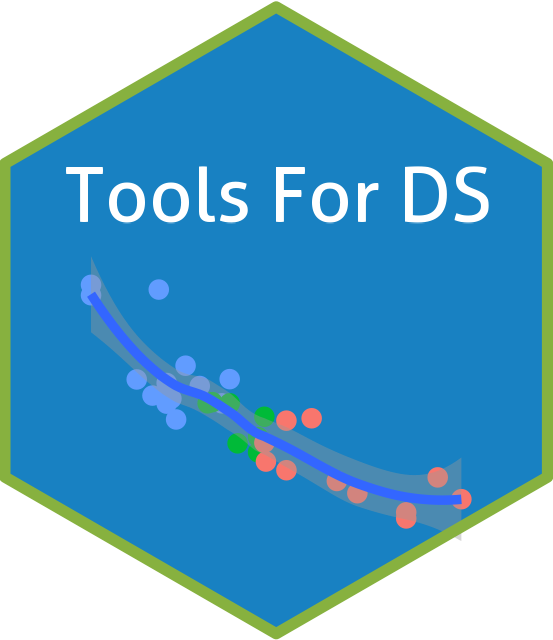
\includegraphics[width=2.72917in,height=\textheight]{logo.png} \hfill{}

\end{figure}

This eBook is used for \textbf{Tools and Statistics for Data Science}
(TS4DS) courses offered at {[}the University of West Florida,
Mathematics and Statistics
Department{]}(https://uwf.edu/hmcse/departments/mathematics-and-statistics/)\{target=``\_blank''\}

An 8-Week course on \textbf{Statistics for data science 1} using R or
SAS.

An 8-Week course on \textbf{Tools for data science} using R, Python, and
SQL. Throughout the course, there will be hands-on exercises with
computing resources. The course will include introductions to several
packages in R, particularly Tidyverse, libraries in Python such as
Pandas/NumPy/Statsmodels, SQL clauses and summary statistics, and Spark
framework for distributed computing.

\hypertarget{topics}{%
\subsection*{Topics}\label{topics}}
\addcontentsline{toc}{subsection}{Topics}

\begin{itemize}
\tightlist
\item
  Introduction to R/RStudio
\item
  Programming using R
\item
  Introduction to Python
\item
  Programming using Python
\item
  Introduction to SQL
\item
  Data input and output
\item
  Data manipulation
\item
  Summary statistics
\item
  Statistical and mathematical functions
\item
  Graphics and data visualization
\item
  Hypothesis testing
\item
  Regression
\item
  t-tests, ANOVA
\item
  Nonparametric tests
\end{itemize}

\hypertarget{readings}{%
\subsection*{Readings}\label{readings}}
\addcontentsline{toc}{subsection}{Readings}

In addition to material provided in this course, I highly encourage
reading and reviewing some of the material, I will be pointing out
throughout the course, including:

\begin{itemize}
\tightlist
\item
  \emph{R for Data Science}
  (\protect\hyperlink{ref-wickham2016r}{Wickham and Grolemund 2016}). It
  is available \href{https://r4ds.had.co.nz/}{free online}.
\item
  \emph{Hands-On Programming with R}
  (\protect\hyperlink{ref-grolemund2014hands}{Grolemund 2014}). It is
  available \href{https://rstudio-education.github.io/hopr/}{free
  online}.
\item
  \emph{Exploring Enterprise Databases with R: A Tidyverse Approach}
  (\protect\hyperlink{ref-databaser2020}{John David et al. 2020})
\item
  \emph{Mastering Spark with R}
  (\protect\hyperlink{ref-luraschi2019mastering}{Luraschi, Kuo, and Ruiz
  2019}). It is available \href{https://therinspark.com/index.html}{free
  online}.
\item
  \emph{Practical Guide for Oracle SQL, T-SQL and MySQL}
  (\protect\hyperlink{ref-zhang2017practical}{Zhang 2017})
\item
  \emph{Think Python} (\protect\hyperlink{ref-Allenpython}{Downey 2015})
\item
  \emph{Data Science and Analytics with Python}
  (\protect\hyperlink{ref-rogel2018data}{Rogel-Salazar 2018})
\end{itemize}

\part{Tools for Data Science}

This is a book created from markdown and executable code.

See (\protect\hyperlink{ref-knuth84}{\textbf{knuth84?}}) for additional
discussion of literate programming.

\begin{Shaded}
\begin{Highlighting}[]
\DecValTok{1} \SpecialCharTok{+} \DecValTok{1}
\end{Highlighting}
\end{Shaded}

\begin{verbatim}
[1] 2
\end{verbatim}

\hypertarget{introduction}{%
\chapter*{Introduction}\label{introduction}}
\addcontentsline{toc}{chapter}{Introduction}

\markboth{Introduction}{Introduction}

An 8-Week course on tools for data science using R, Python, SQL, and
Spark. Throughout the course, there will be hands-on exercises with
computing resources. The course will include introductions to several
packages in R, particularly Tidyverse, libraries in Python such as
Pandas/NumPy/Statsmodels, SQL clauses and summary statistics, and Spark
framework for distributed computing.

\hypertarget{learning-outcomes}{%
\subsection*{Learning outcomes}\label{learning-outcomes}}
\addcontentsline{toc}{subsection}{Learning outcomes}

\begin{itemize}
\tightlist
\item
  Develop programming skills
\item
  Write codes using R, Python, and SQL
\item
  Show the ability to manage, wrangle, and visualize data
\item
  Practice with Spark for distributed processing
\item
  Compare statistical summaries using SQL, R and Python
\item
  Create and evaluate scripts to answer data driven problems
\end{itemize}

\hypertarget{topics-1}{%
\subsection*{Topics}\label{topics-1}}
\addcontentsline{toc}{subsection}{Topics}

\begin{itemize}
\tightlist
\item
  Introduction to R/RStudio
\item
  Programming using R
\item
  Introduction to Python
\item
  Programming using Python
\item
  Introduction to SQL
\item
  Introduction to Spark
\item
  Data input and output
\item
  Data manipulation
\item
  Summary statistics
\item
  Statistical and mathematical functions
\item
  Graphics and data visualization
\end{itemize}

Note that the focus of the course will be learning programming using R
and Python from the very basics. We will explore the usage of SQL and
Spark for querying and processing data. We will learn and practice
coding concepts and programming practices that are universal but
relevant to data science projects and workflow.

\hypertarget{organization-and-evaluation}{%
\subsection*{Organization and
Evaluation}\label{organization-and-evaluation}}
\addcontentsline{toc}{subsection}{Organization and Evaluation}

Each week, we will have 2 tasks to complete as follows:

\begin{longtable}[]{@{}
  >{\raggedright\arraybackslash}p{(\columnwidth - 4\tabcolsep) * \real{0.2917}}
  >{\raggedright\arraybackslash}p{(\columnwidth - 4\tabcolsep) * \real{0.4167}}
  >{\raggedright\arraybackslash}p{(\columnwidth - 4\tabcolsep) * \real{0.2917}}@{}}
\toprule\noalign{}
\begin{minipage}[b]{\linewidth}\raggedright
Days
\end{minipage} & \begin{minipage}[b]{\linewidth}\raggedright
To do
\end{minipage} & \begin{minipage}[b]{\linewidth}\raggedright
Due day
\end{minipage} \\
\midrule\noalign{}
\endhead
\bottomrule\noalign{}
\endlastfoot
Mondays to Wednesdays & Reading/Watch recordings & NA \\
Wednesdays to Mondays & Practice and Discuss (credit 5\%) & Monday@11:59
pm CT \\
& & \\
\end{longtable}

Every two weeks we will have an \textbf{Individual project} (credit
10\%) to complete.

\hypertarget{readings-1}{%
\subsection*{Readings}\label{readings-1}}
\addcontentsline{toc}{subsection}{Readings}

In addition to material provided in this course, I highly encourage
reading and reviewing some of the material, I will be pointing out
throughout the course, including:

\begin{itemize}
\tightlist
\item
  \emph{R for Data Science}
  (\protect\hyperlink{ref-wickham2016r}{Wickham and Grolemund 2016}). It
  is available \href{https://r4ds.had.co.nz/}{free online}.
\item
  \emph{Hands-On Programming with R}
  (\protect\hyperlink{ref-grolemund2014hands}{Grolemund 2014}). It is
  available \href{https://rstudio-education.github.io/hopr/}{free
  online}.
\item
  \emph{Exploring Enterprise Databases with R: A Tidyverse Approach}
  (\protect\hyperlink{ref-databaser2020}{John David et al. 2020})
\item
  \emph{Mastering Spark with R}
  (\protect\hyperlink{ref-luraschi2019mastering}{Luraschi, Kuo, and Ruiz
  2019}). It is available \href{https://therinspark.com/index.html}{free
  online}.
\item
  \emph{Practical Guide for Oracle SQL, T-SQL and MySQL}
  (\protect\hyperlink{ref-zhang2017practical}{Zhang 2017})
\item
  \emph{Think Python} (\protect\hyperlink{ref-Allenpython}{Downey 2015})
\item
  \emph{Data Science and Analytics with Python}
  (\protect\hyperlink{ref-rogel2018data}{Rogel-Salazar 2018})
\end{itemize}

\hypertarget{r-basics}{%
\chapter*{R Basics}\label{r-basics}}
\addcontentsline{toc}{chapter}{R Basics}

\markboth{R Basics}{R Basics}

At the end of this week, you will be able to:

\begin{itemize}
\tightlist
\item
  Show an understanding of data science workflow
\item
  Start your computing environment
\item
  Write your first code using R
\item
  Practice with basic R programming tools such as \texttt{for\ loop},
  \texttt{data\ frames}, etc.
\end{itemize}

\hypertarget{data-science}{%
\section*{Data Science?}\label{data-science}}
\addcontentsline{toc}{section}{Data Science?}

\markright{Data Science?}

The use of data as evidence is crucial but, it is not something novel.
If we examine a definition of the field of \emph{statistics}, we can
observe that is given as four subtopics:

\begin{itemize}
\tightlist
\item
  Data Collection
\item
  Data Analysis
\item
  Results Interpretation
\item
  Data Visualization
\end{itemize}

Originally, \emph{statistics} was viewed as the analysis and
interpretation of information about states. And science is understood as
organized knowledge in the form of testable explanations and predictions
about the universe.

So, what is data science? Data science is more than just using
statistics and data to answer scientific questions.

\begin{quote}
Nowadays, data science is viewed as the use of various sources of data
to extract knowledge and provide insights using multiple skills
including programming, math and statistics, and communication.
\end{quote}

Venn diagram by Drew Conway provides a visualization on data science.

\begin{figure}

{\centering 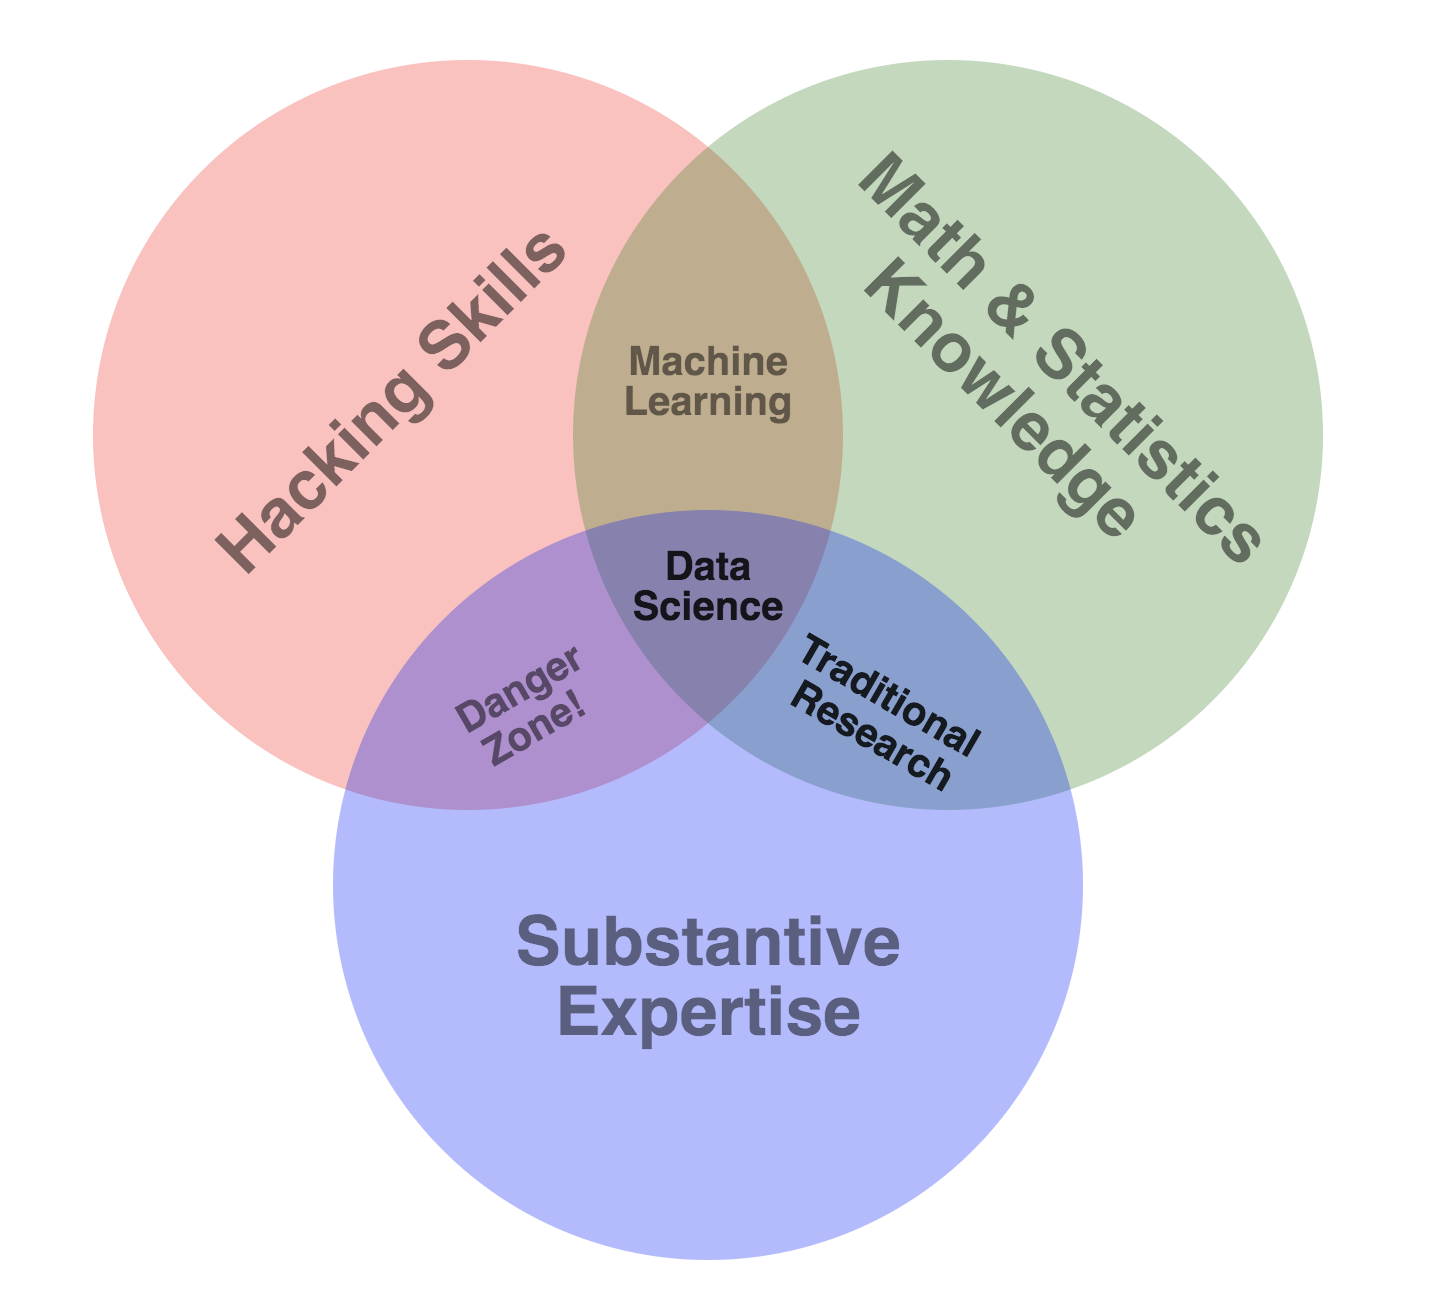
\includegraphics{img/DSvenn.png}

}

\end{figure}

Data Science Venn diagram by Drew Conway

Typical examples of data science projects:

\begin{itemize}
\tightlist
\item
  \textbf{Market analysis} What product will sell better in conjunction
  with another popular product
\item
  \textbf{Market segmentation} Are there distinguishable features that
  characterize different groups of sales agents, customers or
  businesses?
\item
  \textbf{Advertising and marketing} What advertisement should be placed
  on what site?
\item
  \textbf{Fraud} How to detect if a retail/finance transaction is valid
  or not?
\item
  \textbf{Demand forecasting} What is the demand for a particle service
  at a specific time/place?
\item
  \textbf{Classification} Emails classification (spam vs.~valid email)
\end{itemize}

\hypertarget{tools-for-data-science-1}{%
\subsection*{Tools for Data Science}\label{tools-for-data-science-1}}
\addcontentsline{toc}{subsection}{Tools for Data Science}

Data science helps managers, engineers, policymakers, and researchers -
almost everybody - to make informed decisions based on evidence from
data. Computers and technologies have empowered how much data we can
store, manipulate, and analyze. To enable these functions, technologies
and tools are developed to help us to be more productive and efficient
when conducting data science projects.

\begin{figure}

{\centering 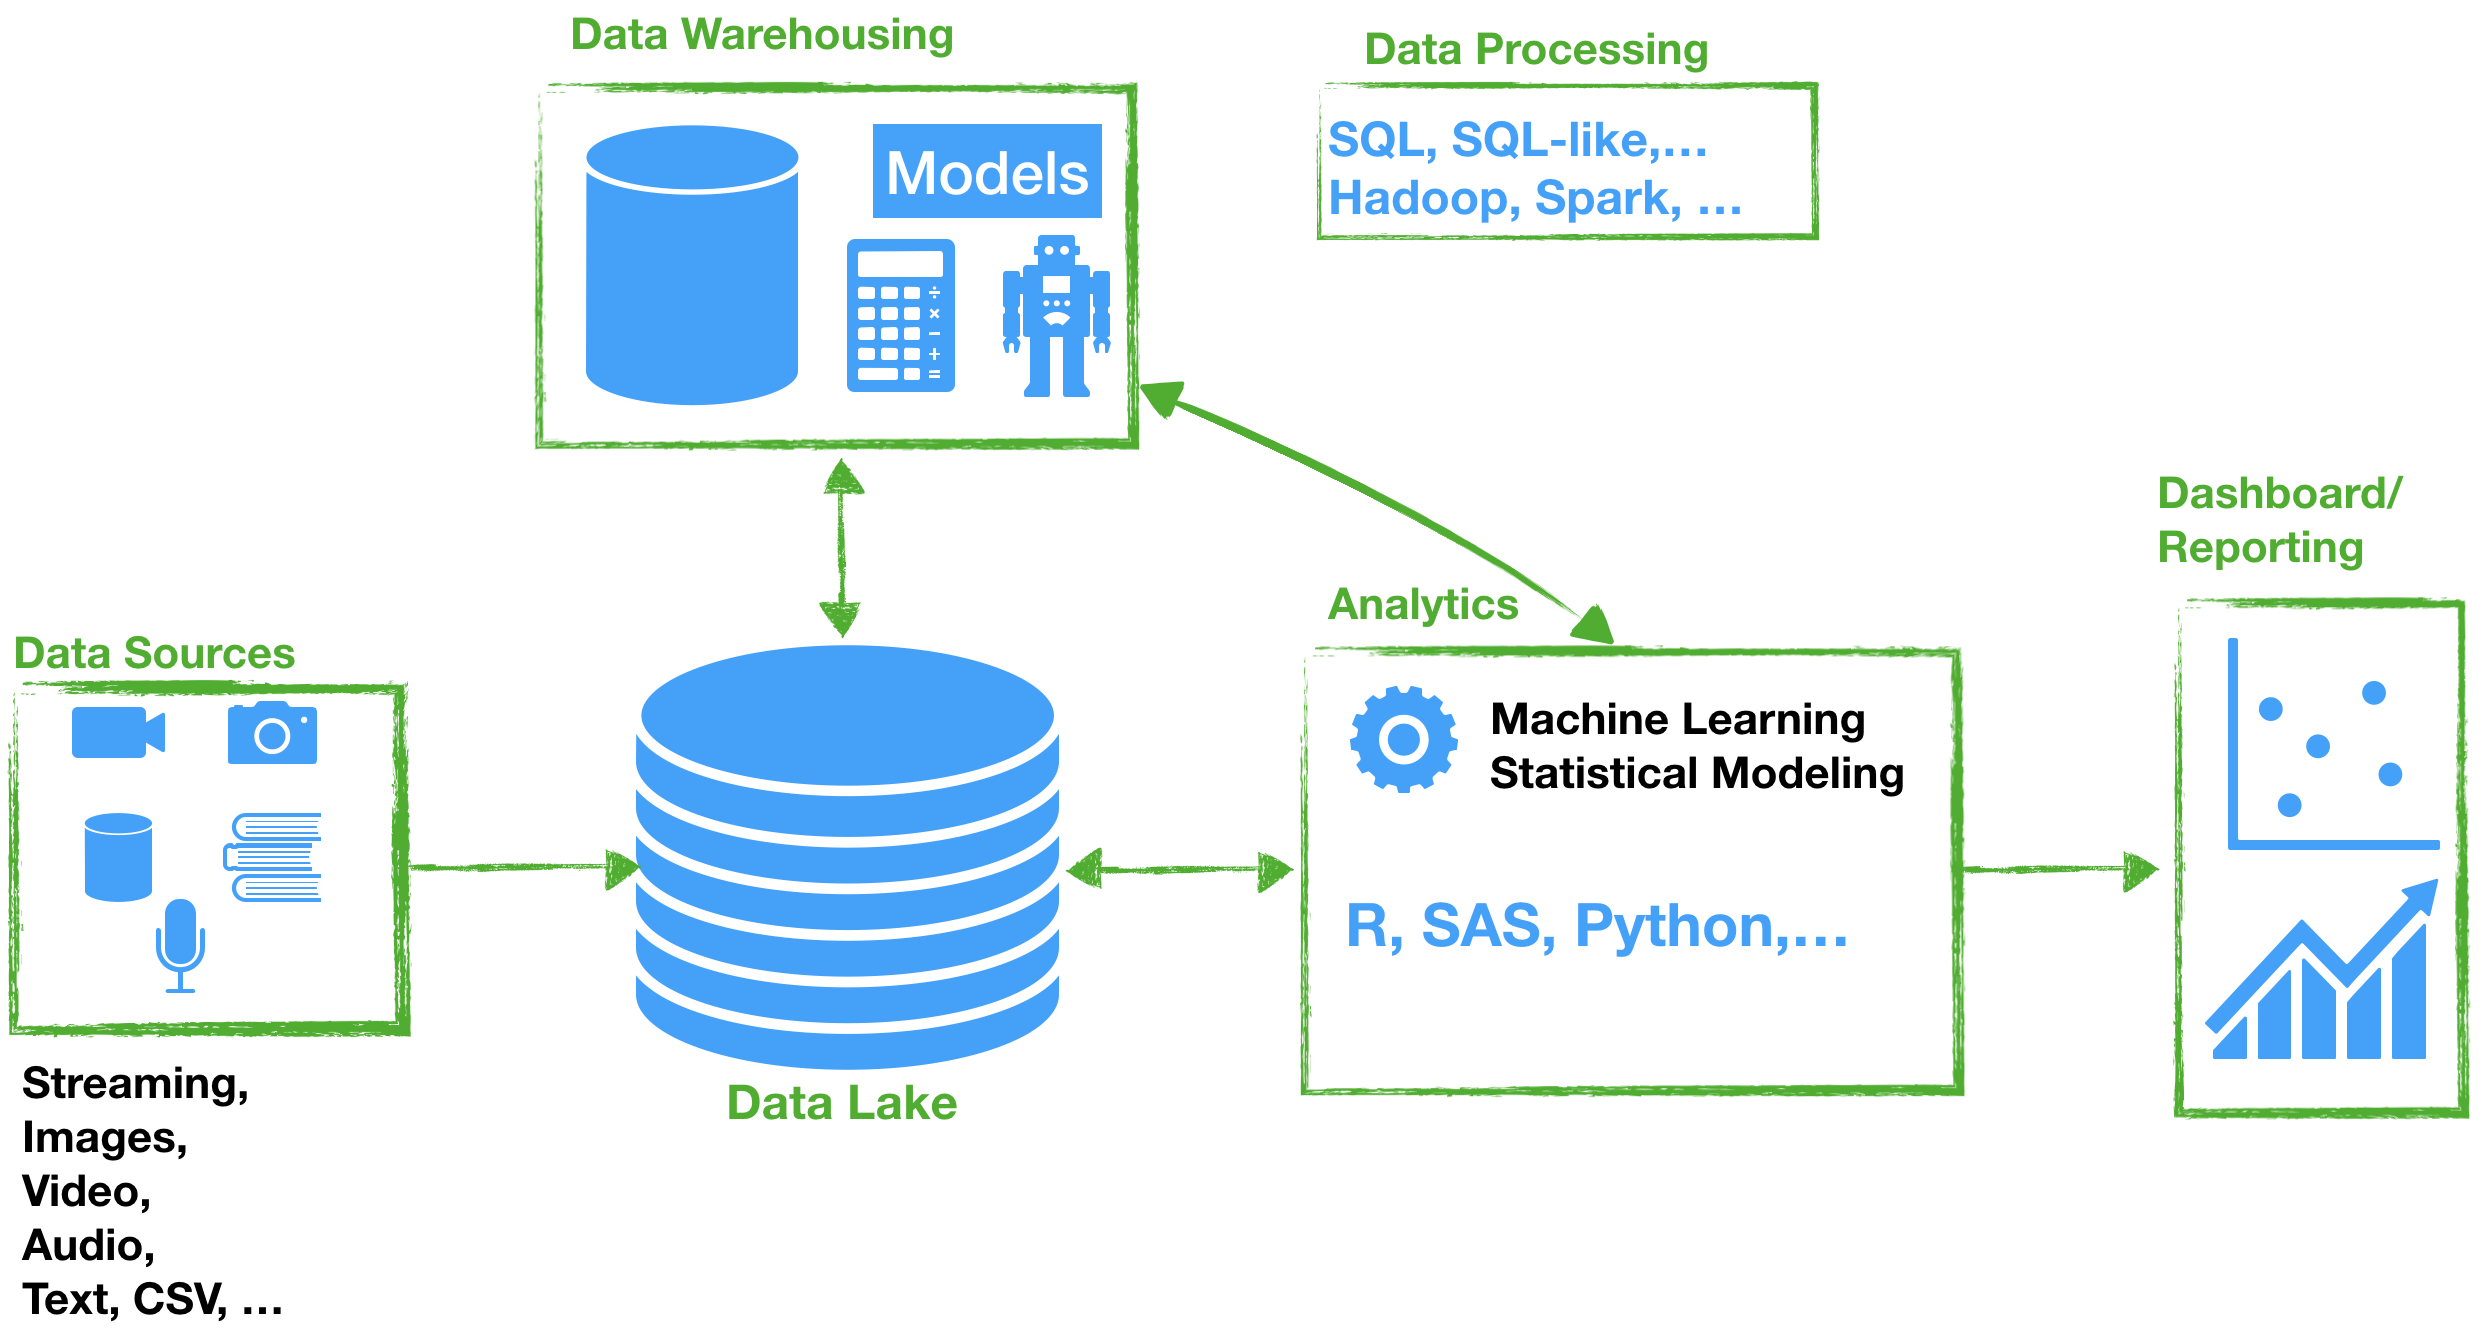
\includegraphics{img/DSWorkflow.png}

}

\caption{Data Science Workflow}

\end{figure}

The technologies deployed in the analytics and data science have
advanced very fast and multiple open source projects exist, for example:

\begin{itemize}
\tightlist
\item
  Data framework: \href{https://hadoop.apache.org/}{Hadoop},
  \href{https://spark.apache.org/}{Spark},\ldots{}
\item
  Query Languages: SQL, SQL-like,\ldots{}
\item
  Data manipulation, modeling, and graphing: R, Python,\ldots{}
\item
  Software management: Git, \href{https://github.com/}{GitHub},\ldots{}
\end{itemize}

\hypertarget{data-science-workflow}{%
\subsection*{Data Science Workflow}\label{data-science-workflow}}
\addcontentsline{toc}{subsection}{Data Science Workflow}

Often, the data science process is iterative. Some steps in the data
science workflow include:

\begin{enumerate}
\def\labelenumi{\arabic{enumi}.}
\tightlist
\item
  Specify the question of interest (business understanding, scientific
  goal, predict or estimate,\ldots)
\item
  Collect data (internal, external, sampled, relevant, ethics,\ldots)
\item
  Manipulate data (explore, transform, merge, filter,\ldots)
\item
  Model data (machine learning, statistics, probability, fit,
  validate,\ldots)
\item
  Communicate and interpret the results (storytelling, visualization,
  dashboard, reports,\ldots)
\item
  Deploy and monitor models
\end{enumerate}

\hypertarget{introduction-to-r-rstudio}{%
\section*{Introduction to R / RStudio}\label{introduction-to-r-rstudio}}
\addcontentsline{toc}{section}{Introduction to R / RStudio}

\markright{Introduction to R / RStudio}

The two programming languages we cover in this course are R and Python.
These are both open source programming languages. Let's start off with
R.

A few features of R are:

\begin{quote}
\begin{itemize}
\tightlist
\item
  \textbf{R} is a free software environment for statistical computing
  and graphics.
\item
  It compiles and runs on a wide variety of UNIX platforms, Windows and
  MacOS.
\item
  \href{https://www.r-project.org/}{The R project website} contains a
  lot of useful information about:
  \href{https://cran.r-project.org/mirrors.html}{download R},
  documentation and
  \href{https://cran.r-project.org/manuals.html}{manuals},
  \href{https://journal.r-project.org/}{The R journal},
  \href{https://www.r-project.org/doc/bib/R-books.html}{books related to
  R}, and \href{https://cran.r-project.org/web/views/}{R packages by
  topics}
\item
  There is a large active community of R users.
\end{itemize}
\end{quote}

\begin{quote}
\textbf{RStudio} is an integrated development environment (IDE) for R
and Python, with a console, syntax-highlighting editor that supports
direct code execution, and tools for plotting, history, debugging and
workspace management. It compiles and runs on a wide variety of UNIX
platforms, Windows and MacOS. \href{https://www.rstudio.com/}{The
RStudio website}. There is an open source license for both the desktop
and server versions that you install for free from here:
\href{https://www.rstudio.com/products/rstudio/download/}{download
RStudio}
\end{quote}

\begin{quote}
\textbf{R Markdown} provides an authoring framework for data science.
You can use a single R Markdown file to both save and execute code
generate high quality reports that can be shared with an audience. R
Markdown documents are fully reproducible and support dozens of static
and dynamic output formats.
\href{https://rmarkdown.rstudio.com/lesson-1.html}{The R Markdown
1-minute video} provides an overview of what R Markdown can do!
\end{quote}

\hypertarget{install-your-rrstudio}{%
\subsubsection*{Install your R/RStudio}\label{install-your-rrstudio}}
\addcontentsline{toc}{subsubsection}{Install your R/RStudio}

For TFDS, we will be using RStudio Server hosted at
\href{https://uwf.edu}{UWF}. This is the link
\url{https://rstudio.hmcse.uwf.edu/}. \textbf{Login using your UWF
account}.

You don't need to install R and RStudio on your computer. But, you are
welcome to do so if you wish so.

\hypertarget{getting-started-with-r}{%
\section*{Getting started with R}\label{getting-started-with-r}}
\addcontentsline{toc}{section}{Getting started with R}

\markright{Getting started with R}

🛎️ Recordings of this week provide lessons about R, RStudio, and GitHub.
The following will be covered:

\begin{itemize}
\tightlist
\item
  RStudio (editor, console, global Env., and etc.)
\item
  R (scripts, packages, help)
\item
  GitHub and connection to RStudio
\item
  R Markdown - \href{https://www.markdownguide.org/cheat-sheet/}{Cheet
  Sheet}
\item
  My first R script - the basics

  \begin{itemize}
  \tightlist
  \item
    Values, vectors, matrices, factors, data.frames, lists. Here is an
    example of code:
  \end{itemize}
\end{itemize}

\begin{Shaded}
\begin{Highlighting}[]
\CommentTok{\# assign a value to object named "x"}
\NormalTok{x }\OtherTok{=} \DecValTok{1}
\CommentTok{\# or}
\NormalTok{x }\OtherTok{\textless{}{-}} \DecValTok{1}
\DecValTok{1} \OtherTok{{-}\textgreater{}}\NormalTok{ x  }
\CommentTok{\# Calculator }
\NormalTok{x}\OtherTok{=}\DecValTok{10}\SpecialCharTok{\^{}}\DecValTok{2}
\NormalTok{y}\OtherTok{=}\DecValTok{2}\SpecialCharTok{*}\NormalTok{x}
\CommentTok{\# vectors}
\FunctionTok{c}\NormalTok{(}\DecValTok{1}\NormalTok{,}\DecValTok{21}\NormalTok{,}\DecValTok{50}\NormalTok{,}\DecValTok{80}\NormalTok{,}\DecValTok{45}\NormalTok{,}\DecValTok{0}\NormalTok{)}
\end{Highlighting}
\end{Shaded}

\begin{verbatim}
[1]  1 21 50 80 45  0
\end{verbatim}

\begin{Shaded}
\begin{Highlighting}[]
\FunctionTok{c}\NormalTok{(}\StringTok{"d"}\NormalTok{,}\StringTok{"4"}\NormalTok{,}\StringTok{"r"}\NormalTok{)}
\end{Highlighting}
\end{Shaded}

\begin{verbatim}
[1] "d" "4" "r"
\end{verbatim}

\begin{Shaded}
\begin{Highlighting}[]
\CommentTok{\# characters}
\StringTok{"R is useful and cool"}
\end{Highlighting}
\end{Shaded}

\begin{verbatim}
[1] "R is useful and cool"
\end{verbatim}

\begin{Shaded}
\begin{Highlighting}[]
\CommentTok{\# boolean {-} TRUE or FALSE}
\DecValTok{45}\SpecialCharTok{\textgreater{}}\DecValTok{96}
\end{Highlighting}
\end{Shaded}

\begin{verbatim}
[1] FALSE
\end{verbatim}

\begin{Shaded}
\begin{Highlighting}[]
\CommentTok{\# built{-}in functions}
\FunctionTok{sum}\NormalTok{(}\DecValTok{1}\NormalTok{,}\DecValTok{3}\NormalTok{,}\DecValTok{5}\NormalTok{)}
\end{Highlighting}
\end{Shaded}

\begin{verbatim}
[1] 9
\end{verbatim}

\begin{itemize}
\tightlist
\item
  Statistical and mathematical functions: An example of code:
\end{itemize}

\begin{Shaded}
\begin{Highlighting}[]
\CommentTok{\# a vector / array}
\NormalTok{vec1}\OtherTok{=} \FunctionTok{c}\NormalTok{(}\DecValTok{1}\NormalTok{,}\DecValTok{21}\NormalTok{,}\DecValTok{50}\NormalTok{,}\DecValTok{80}\NormalTok{,}\DecValTok{45}\NormalTok{,}\DecValTok{0}\NormalTok{)}
\CommentTok{\# minimun}
\FunctionTok{min}\NormalTok{(vec1)}
\end{Highlighting}
\end{Shaded}

\begin{verbatim}
[1] 0
\end{verbatim}

\begin{Shaded}
\begin{Highlighting}[]
\CommentTok{\# maximum}
\FunctionTok{max}\NormalTok{(vec1)}
\end{Highlighting}
\end{Shaded}

\begin{verbatim}
[1] 80
\end{verbatim}

\begin{Shaded}
\begin{Highlighting}[]
\CommentTok{\# exponential function}
\FunctionTok{exp}\NormalTok{(vec1)}
\end{Highlighting}
\end{Shaded}

\begin{verbatim}
[1] 2.718282e+00 1.318816e+09 5.184706e+21 5.540622e+34 3.493427e+19
[6] 1.000000e+00
\end{verbatim}

\begin{Shaded}
\begin{Highlighting}[]
\CommentTok{\# cosine function}
\FunctionTok{cos}\NormalTok{(vec1)}
\end{Highlighting}
\end{Shaded}

\begin{verbatim}
[1]  0.5403023 -0.5477293  0.9649660 -0.1103872  0.5253220  1.0000000
\end{verbatim}

\begin{Shaded}
\begin{Highlighting}[]
\CommentTok{\# sine function}
\FunctionTok{sin}\NormalTok{(vec1)}
\end{Highlighting}
\end{Shaded}

\begin{verbatim}
[1]  0.8414710  0.8366556 -0.2623749 -0.9938887  0.8509035  0.0000000
\end{verbatim}

\begin{Shaded}
\begin{Highlighting}[]
\CommentTok{\# logarithm function of base e}
\FunctionTok{log}\NormalTok{(vec1,}\FloatTok{0.5}\NormalTok{)}
\end{Highlighting}
\end{Shaded}

\begin{verbatim}
[1]  0.000000 -4.392317 -5.643856 -6.321928 -5.491853       Inf
\end{verbatim}

\begin{Shaded}
\begin{Highlighting}[]
\CommentTok{\# square root}
\FunctionTok{sqrt}\NormalTok{(vec1)}
\end{Highlighting}
\end{Shaded}

\begin{verbatim}
[1] 1.000000 4.582576 7.071068 8.944272 6.708204 0.000000
\end{verbatim}

\begin{Shaded}
\begin{Highlighting}[]
\CommentTok{\# logarithm function of base 10}
\FunctionTok{log10}\NormalTok{(}\DecValTok{10}\NormalTok{)}
\end{Highlighting}
\end{Shaded}

\begin{verbatim}
[1] 1
\end{verbatim}

\begin{Shaded}
\begin{Highlighting}[]
\CommentTok{\# logarithm function of base 2}
\FunctionTok{log2}\NormalTok{(}\DecValTok{2}\NormalTok{)}
\end{Highlighting}
\end{Shaded}

\begin{verbatim}
[1] 1
\end{verbatim}

\begin{Shaded}
\begin{Highlighting}[]
\CommentTok{\# logarithm function of base 45}
\FunctionTok{log}\NormalTok{(}\DecValTok{45}\NormalTok{,}\AttributeTok{base =} \DecValTok{45}\NormalTok{)}
\end{Highlighting}
\end{Shaded}

\begin{verbatim}
[1] 1
\end{verbatim}

\begin{Shaded}
\begin{Highlighting}[]
\CommentTok{\# factorial}
\FunctionTok{factorial}\NormalTok{(}\DecValTok{3}\NormalTok{)}
\end{Highlighting}
\end{Shaded}

\begin{verbatim}
[1] 6
\end{verbatim}

\begin{Shaded}
\begin{Highlighting}[]
\CommentTok{\# binomial coefficient / combination}
\FunctionTok{choose}\NormalTok{(}\DecValTok{10}\NormalTok{,}\DecValTok{5}\NormalTok{)}
\end{Highlighting}
\end{Shaded}

\begin{verbatim}
[1] 252
\end{verbatim}

\begin{itemize}
\tightlist
\item
  Summary statistics, random number generation. An example:
\end{itemize}

\begin{Shaded}
\begin{Highlighting}[]
\CommentTok{\# a set of values}
\NormalTok{vec1}\OtherTok{=} \FunctionTok{c}\NormalTok{(}\DecValTok{1}\NormalTok{,}\DecValTok{21}\NormalTok{,}\DecValTok{50}\NormalTok{,}\DecValTok{80}\NormalTok{,}\DecValTok{45}\NormalTok{,}\DecValTok{0}\NormalTok{)}
\CommentTok{\# summation}
\FunctionTok{sum}\NormalTok{(vec1)}
\end{Highlighting}
\end{Shaded}

\begin{verbatim}
[1] 197
\end{verbatim}

\begin{Shaded}
\begin{Highlighting}[]
\CommentTok{\# arithmetic mean}
\FunctionTok{mean}\NormalTok{(vec1)}
\end{Highlighting}
\end{Shaded}

\begin{verbatim}
[1] 32.83333
\end{verbatim}

\begin{Shaded}
\begin{Highlighting}[]
\CommentTok{\# standard deviation}
\FunctionTok{sd}\NormalTok{(vec1)}
\end{Highlighting}
\end{Shaded}

\begin{verbatim}
[1] 31.30122
\end{verbatim}

\begin{Shaded}
\begin{Highlighting}[]
\CommentTok{\# summary statistics}
\FunctionTok{summary}\NormalTok{(vec1)}
\end{Highlighting}
\end{Shaded}

\begin{verbatim}
   Min. 1st Qu.  Median    Mean 3rd Qu.    Max. 
   0.00    6.00   33.00   32.83   48.75   80.00 
\end{verbatim}

\begin{Shaded}
\begin{Highlighting}[]
\CommentTok{\# variance}
\FunctionTok{var}\NormalTok{(vec1)}
\end{Highlighting}
\end{Shaded}

\begin{verbatim}
[1] 979.7667
\end{verbatim}

\begin{Shaded}
\begin{Highlighting}[]
\CommentTok{\# quantile}
\FunctionTok{quantile}\NormalTok{(vec1,}\FloatTok{0.5}\NormalTok{)}
\end{Highlighting}
\end{Shaded}

\begin{verbatim}
50% 
 33 
\end{verbatim}

\begin{Shaded}
\begin{Highlighting}[]
\CommentTok{\# 100 Standard normal random numbers}
\NormalTok{x}\OtherTok{=}\FunctionTok{rnorm}\NormalTok{(}\DecValTok{100}\NormalTok{,}\AttributeTok{mean=}\DecValTok{0}\NormalTok{,}\AttributeTok{sd=}\DecValTok{1}\NormalTok{)}
\CommentTok{\# histogram}
\FunctionTok{hist}\NormalTok{(x)}
\end{Highlighting}
\end{Shaded}

\begin{figure}[H]

{\centering 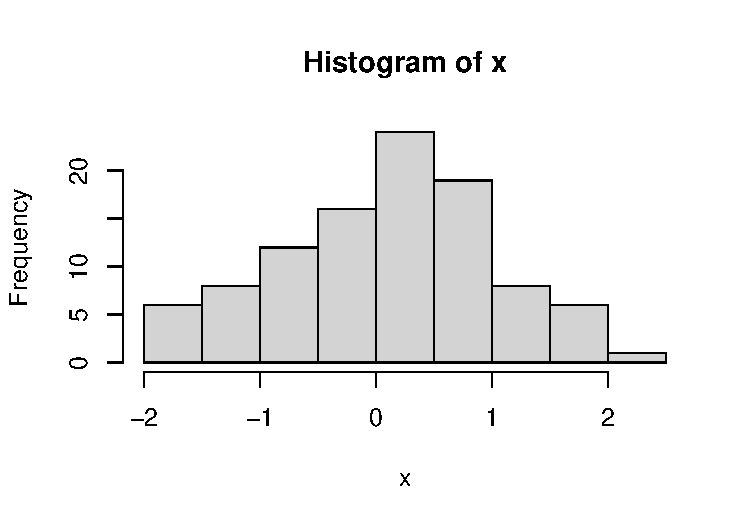
\includegraphics{t4ds/week1_files/figure-pdf/unnamed-chunk-3-1.pdf}

}

\end{figure}

\begin{itemize}
\tightlist
\item
  Functions, conditional statements: \emph{if}, \emph{for} and
  \emph{while}. A code example:
\end{itemize}

\begin{Shaded}
\begin{Highlighting}[]
\CommentTok{\# create your own function}
\NormalTok{  myfunction}\OtherTok{=}\ControlFlowTok{function}\NormalTok{()\{}
    \FunctionTok{return}\NormalTok{(}\FunctionTok{print}\NormalTok{(}\StringTok{"Hello there!"}\NormalTok{))}
\NormalTok{  \}}
\CommentTok{\# if statement}
\NormalTok{lucky.number}\OtherTok{=}\DecValTok{100}
\ControlFlowTok{if}\NormalTok{(lucky.number}\SpecialCharTok{\textless{}=}\DecValTok{54}\NormalTok{)\{}
\FunctionTok{print}\NormalTok{(}\StringTok{"You win!"}\NormalTok{)}
\NormalTok{  \}}\ControlFlowTok{else}\NormalTok{\{}
  \FunctionTok{print}\NormalTok{(}\StringTok{"You lost!"}\NormalTok{)}
\NormalTok{\}}
\end{Highlighting}
\end{Shaded}

\begin{verbatim}
[1] "You lost!"
\end{verbatim}

🛎 🎙️ Recordings on Canvas will cover more details and examples! Have fun
learning and coding 😃! Let me know how I can help!

\hypertarget{assignment---r-basics}{%
\section*{📚 👈 Assignment - R basics}\label{assignment---r-basics}}
\addcontentsline{toc}{section}{📚 👈 Assignment - R basics}

\markright{📚 👈 Assignment - R basics}

Instructions are posted on Canvas.

\hypertarget{r-tidyverse}{%
\chapter*{R Tidyverse}\label{r-tidyverse}}
\addcontentsline{toc}{chapter}{R Tidyverse}

\markboth{R Tidyverse}{R Tidyverse}

At the end of this week, you will be able to:

\begin{itemize}
\tightlist
\item
  Use R packages especially \href{https://www.tidyverse.org/}{Tidyverse}
\item
  Identify \texttt{Tidy} data
\item
  Practice with pipe operator \texttt{\%\textgreater{}\%},
  \texttt{select()}, \texttt{filter()},\ldots{} for data wrangling
\item
  Visualization using \texttt{ggplot2} package.
\end{itemize}

All \href{https://www.rstudio.com/resources/cheatsheets/}{Cheat Sheets}
are very useful!

\hypertarget{tidy-data}{%
\section*{Tidy data}\label{tidy-data}}
\addcontentsline{toc}{section}{Tidy data}

\markright{Tidy data}

A data is said to be
\href{https://vita.had.co.nz/papers/tidy-data.html}{tidy}
(\protect\hyperlink{ref-tidy-data}{Wickham 2014}) format if each column
represents a variable and each row represents an observation. Example of
data that is \emph{NOT} \texttt{tidy} is the \texttt{relig\_income} data
set in \texttt{tidyr} package:

\begin{Shaded}
\begin{Highlighting}[]
\CommentTok{\# load a libraries}
\FunctionTok{library}\NormalTok{(knitr) }\CommentTok{\# fancy table}
\FunctionTok{library}\NormalTok{(tidyverse) }\CommentTok{\# load library tidyverse}
\CommentTok{\# To display fancy tables}
\FunctionTok{kable}\NormalTok{(}\FunctionTok{head}\NormalTok{(relig\_income,}\DecValTok{10}\NormalTok{))}
\end{Highlighting}
\end{Shaded}

\begin{longtable}[]{@{}
  >{\raggedright\arraybackslash}p{(\columnwidth - 20\tabcolsep) * \real{0.2105}}
  >{\raggedleft\arraybackslash}p{(\columnwidth - 20\tabcolsep) * \real{0.0526}}
  >{\raggedleft\arraybackslash}p{(\columnwidth - 20\tabcolsep) * \real{0.0702}}
  >{\raggedleft\arraybackslash}p{(\columnwidth - 20\tabcolsep) * \real{0.0702}}
  >{\raggedleft\arraybackslash}p{(\columnwidth - 20\tabcolsep) * \real{0.0702}}
  >{\raggedleft\arraybackslash}p{(\columnwidth - 20\tabcolsep) * \real{0.0702}}
  >{\raggedleft\arraybackslash}p{(\columnwidth - 20\tabcolsep) * \real{0.0702}}
  >{\raggedleft\arraybackslash}p{(\columnwidth - 20\tabcolsep) * \real{0.0789}}
  >{\raggedleft\arraybackslash}p{(\columnwidth - 20\tabcolsep) * \real{0.0877}}
  >{\raggedleft\arraybackslash}p{(\columnwidth - 20\tabcolsep) * \real{0.0526}}
  >{\raggedleft\arraybackslash}p{(\columnwidth - 20\tabcolsep) * \real{0.1667}}@{}}
\toprule\noalign{}
\begin{minipage}[b]{\linewidth}\raggedright
religion
\end{minipage} & \begin{minipage}[b]{\linewidth}\raggedleft
\textless\$10k
\end{minipage} & \begin{minipage}[b]{\linewidth}\raggedleft
\$10-20k
\end{minipage} & \begin{minipage}[b]{\linewidth}\raggedleft
\$20-30k
\end{minipage} & \begin{minipage}[b]{\linewidth}\raggedleft
\$30-40k
\end{minipage} & \begin{minipage}[b]{\linewidth}\raggedleft
\$40-50k
\end{minipage} & \begin{minipage}[b]{\linewidth}\raggedleft
\$50-75k
\end{minipage} & \begin{minipage}[b]{\linewidth}\raggedleft
\$75-100k
\end{minipage} & \begin{minipage}[b]{\linewidth}\raggedleft
\$100-150k
\end{minipage} & \begin{minipage}[b]{\linewidth}\raggedleft
\textgreater150k
\end{minipage} & \begin{minipage}[b]{\linewidth}\raggedleft
Don't know/refused
\end{minipage} \\
\midrule\noalign{}
\endhead
\bottomrule\noalign{}
\endlastfoot
Agnostic & 27 & 34 & 60 & 81 & 76 & 137 & 122 & 109 & 84 & 96 \\
Atheist & 12 & 27 & 37 & 52 & 35 & 70 & 73 & 59 & 74 & 76 \\
Buddhist & 27 & 21 & 30 & 34 & 33 & 58 & 62 & 39 & 53 & 54 \\
Catholic & 418 & 617 & 732 & 670 & 638 & 1116 & 949 & 792 & 633 &
1489 \\
Don't know/refused & 15 & 14 & 15 & 11 & 10 & 35 & 21 & 17 & 18 & 116 \\
Evangelical Prot & 575 & 869 & 1064 & 982 & 881 & 1486 & 949 & 723 & 414
& 1529 \\
Hindu & 1 & 9 & 7 & 9 & 11 & 34 & 47 & 48 & 54 & 37 \\
Historically Black Prot & 228 & 244 & 236 & 238 & 197 & 223 & 131 & 81 &
78 & 339 \\
Jehovah's Witness & 20 & 27 & 24 & 24 & 21 & 30 & 15 & 11 & 6 & 37 \\
Jewish & 19 & 19 & 25 & 25 & 30 & 95 & 69 & 87 & 151 & 162 \\
\end{longtable}

It is obvious that each column does not represent a variable. Variable
\texttt{salary} could be a better fit to the values we have in the
columns headings (\textless\$10k, etc.). Another variable can be created
to store values in the entry table (27, 34,\ldots). These are the number
of time we have a response - counts -. To make it \texttt{tidy} we need
then to \emph{pivot} the values columns into a two-column key-value
pair. Let's name the values in the header \texttt{income} and values in
the table \texttt{counts.} To do that we can run the following code:

\begin{Shaded}
\begin{Highlighting}[]
\CommentTok{\# pivot a table/data frame}
\FunctionTok{pivot\_longer}\NormalTok{(relig\_income,}\SpecialCharTok{{-}}\NormalTok{religion,}\AttributeTok{names\_to=}\StringTok{\textquotesingle{}income\textquotesingle{}}\NormalTok{,}\AttributeTok{values\_to =} \StringTok{"count"}\NormalTok{) }\OtherTok{{-}\textgreater{}}\NormalTok{ tidydata}
\CommentTok{\# To display fancy tables}
\FunctionTok{kable}\NormalTok{(}\FunctionTok{head}\NormalTok{(tidydata,}\AttributeTok{n =} \DecValTok{12}\NormalTok{))}
\end{Highlighting}
\end{Shaded}

\begin{longtable}[]{@{}llr@{}}
\toprule\noalign{}
religion & income & count \\
\midrule\noalign{}
\endhead
\bottomrule\noalign{}
\endlastfoot
Agnostic & \textless\$10k & 27 \\
Agnostic & \$10-20k & 34 \\
Agnostic & \$20-30k & 60 \\
Agnostic & \$30-40k & 81 \\
Agnostic & \$40-50k & 76 \\
Agnostic & \$50-75k & 137 \\
Agnostic & \$75-100k & 122 \\
Agnostic & \$100-150k & 109 \\
Agnostic & \textgreater150k & 84 \\
Agnostic & Don't know/refused & 96 \\
Atheist & \textless\$10k & 12 \\
Atheist & \$10-20k & 27 \\
\end{longtable}

\hypertarget{manipulating-data}{%
\section*{Manipulating data}\label{manipulating-data}}
\addcontentsline{toc}{section}{Manipulating data}

\markright{Manipulating data}

\texttt{dplyr} package is designed to perform some of the widely used
operations when working with \texttt{data.frame} or \texttt{tibble}. -
The
\href{https://www.rstudio.com/wp-content/uploads/2015/02/data-wrangling-cheatsheet.pdf}{\texttt{dplyr}
Cheet Sheet}. When manipulating data, you may want to:

\begin{itemize}
\tightlist
\item
  Subset the data to contain only row (observations) you are interested
  in
\item
  Subset the data to contain only columns (variables) you are interested
  in
\item
  Create new variables and add them to the data
\item
  aggregate the data
\end{itemize}

To achieve these operations and more, the package \texttt{dplyr}offers
the following functions:

\begin{longtable}[]{@{}ll@{}}
\toprule\noalign{}
Function & Action \\
\midrule\noalign{}
\endhead
\bottomrule\noalign{}
\endlastfoot
filter() & subset rows \\
select() & subset variables \\
mutate() & create a new variable \\
arrange() & sort \\
summarize() & aggregate the data \\
---------- & --------- \\
\end{longtable}

Here is an example:

\begin{Shaded}
\begin{Highlighting}[]
\CommentTok{\# pivot a table/data frame}
\FunctionTok{pivot\_longer}\NormalTok{(relig\_income,}\SpecialCharTok{{-}}\NormalTok{religion,}\AttributeTok{names\_to=}\StringTok{\textquotesingle{}income\textquotesingle{}}\NormalTok{,}\AttributeTok{values\_to =} \StringTok{"count"}\NormalTok{) }\OtherTok{{-}\textgreater{}}\NormalTok{ tidydata}
\CommentTok{\# Select data where income is \textless{} $10k}
\FunctionTok{kable}\NormalTok{(}\FunctionTok{head}\NormalTok{(}\FunctionTok{filter}\NormalTok{(tidydata,income}\SpecialCharTok{==}\StringTok{"\textless{}$10k"}\NormalTok{)))}
\end{Highlighting}
\end{Shaded}

\begin{longtable}[]{@{}llr@{}}
\toprule\noalign{}
religion & income & count \\
\midrule\noalign{}
\endhead
\bottomrule\noalign{}
\endlastfoot
Agnostic & \textless\$10k & 27 \\
Atheist & \textless\$10k & 12 \\
Buddhist & \textless\$10k & 27 \\
Catholic & \textless\$10k & 418 \\
Don't know/refused & \textless\$10k & 15 \\
Evangelical Prot & \textless\$10k & 575 \\
\end{longtable}

\begin{Shaded}
\begin{Highlighting}[]
\CommentTok{\# Select data where income is \textless{} $10k}
\FunctionTok{kable}\NormalTok{(}\FunctionTok{head}\NormalTok{(}\FunctionTok{arrange}\NormalTok{(tidydata,}\FunctionTok{desc}\NormalTok{(count))))}
\end{Highlighting}
\end{Shaded}

\begin{longtable}[]{@{}llr@{}}
\toprule\noalign{}
religion & income & count \\
\midrule\noalign{}
\endhead
\bottomrule\noalign{}
\endlastfoot
Evangelical Prot & Don't know/refused & 1529 \\
Catholic & Don't know/refused & 1489 \\
Evangelical Prot & \$50-75k & 1486 \\
Mainline Prot & Don't know/refused & 1328 \\
Catholic & \$50-75k & 1116 \\
Mainline Prot & \$50-75k & 1107 \\
\end{longtable}

\hypertarget{pipe-operator}{%
\section*{\texorpdfstring{Pipe operator
\texttt{\%\textgreater{}\%}}{Pipe operator \%\textgreater\%}}\label{pipe-operator}}
\addcontentsline{toc}{section}{Pipe operator
\texttt{\%\textgreater{}\%}}

\markright{Pipe operator \texttt{\%\textgreater{}\%}}

The pipe operator \texttt{\%\textgreater{}\%} allows us to perform a
series of functions without storing the outcomes of each function. For
example:

\begin{Shaded}
\begin{Highlighting}[]
\FunctionTok{library}\NormalTok{(dplyr)}
\FunctionTok{sqrt}\NormalTok{(}\FunctionTok{log}\NormalTok{(}\DecValTok{25}\NormalTok{))}
\end{Highlighting}
\end{Shaded}

{[}1{]} 1.794123

\begin{Shaded}
\begin{Highlighting}[]
\CommentTok{\#is the same as}
\DecValTok{25} \SpecialCharTok{\%\textgreater{}\%} 
\NormalTok{  log }\SpecialCharTok{\%\textgreater{}\%} 
\NormalTok{  sqrt}
\end{Highlighting}
\end{Shaded}

{[}1{]} 1.794123

We often start with our data and then apply functions sequentially. The
benefit of the pipe operator is more evident when dealing with complex
operations.

\hypertarget{summarizing-data}{%
\section*{Summarizing data}\label{summarizing-data}}
\addcontentsline{toc}{section}{Summarizing data}

\markright{Summarizing data}

One of the tasks in statistics is to summarize data. Let's look into
this example using data \texttt{chickwts} about Chicken weights and
diet. It has two variables \texttt{weight} and \texttt{feed}:

\begin{Shaded}
\begin{Highlighting}[]
\CommentTok{\# See what is in the data}
\FunctionTok{str}\NormalTok{(chickwts)}
\end{Highlighting}
\end{Shaded}

\begin{verbatim}
'data.frame':   71 obs. of  2 variables:
 $ weight: num  179 160 136 227 217 168 108 124 143 140 ...
 $ feed  : Factor w/ 6 levels "casein","horsebean",..: 2 2 2 2 2 2 2 2 2 2 ...
\end{verbatim}

\begin{Shaded}
\begin{Highlighting}[]
\CommentTok{\# Mean and standard deviation of the weight}
\NormalTok{chickwts }\SpecialCharTok{\%\textgreater{}\%} 
  \FunctionTok{summarise}\NormalTok{(}\AttributeTok{mean.weight=}\FunctionTok{mean}\NormalTok{(weight),}\AttributeTok{s.weight=}\FunctionTok{sd}\NormalTok{(weight))}
\end{Highlighting}
\end{Shaded}

\begin{verbatim}
  mean.weight s.weight
1    261.3099  78.0737
\end{verbatim}

\begin{Shaded}
\begin{Highlighting}[]
\CommentTok{\# Mean and standard deviation of the weight by group}
\NormalTok{chickwts }\SpecialCharTok{\%\textgreater{}\%} 
  \FunctionTok{group\_by}\NormalTok{(feed) }\SpecialCharTok{\%\textgreater{}\%} 
  \FunctionTok{summarise}\NormalTok{(}\AttributeTok{mean.weight=}\FunctionTok{mean}\NormalTok{(weight),}\AttributeTok{s.weight=}\FunctionTok{sd}\NormalTok{(weight), }\AttributeTok{nbr.chick=}\FunctionTok{n}\NormalTok{())}
\end{Highlighting}
\end{Shaded}

\begin{verbatim}
# A tibble: 6 x 4
  feed      mean.weight s.weight nbr.chick
  <fct>           <dbl>    <dbl>     <int>
1 casein           324.     64.4        12
2 horsebean        160.     38.6        10
3 linseed          219.     52.2        12
4 meatmeal         277.     64.9        11
5 soybean          246.     54.1        14
6 sunflower        329.     48.8        12
\end{verbatim}

\begin{Shaded}
\begin{Highlighting}[]
\CommentTok{\# Select groups \textasciigrave{}casein\textasciigrave{}, \textasciigrave{}linseed\textasciigrave{}, and \textasciigrave{}soybean\textasciigrave{}}
\NormalTok{chickwts }\SpecialCharTok{\%\textgreater{}\%} 
  \FunctionTok{filter}\NormalTok{(feed }\SpecialCharTok{\%in\%} \FunctionTok{c}\NormalTok{(}\StringTok{"casein"}\NormalTok{,}\StringTok{"linseed"}\NormalTok{,}\StringTok{"soybean"}\NormalTok{)) }\SpecialCharTok{\%\textgreater{}\%} 
  \FunctionTok{group\_by}\NormalTok{(feed) }\SpecialCharTok{\%\textgreater{}\%} 
  \FunctionTok{summarise}\NormalTok{(}\AttributeTok{mean.weight=}\FunctionTok{mean}\NormalTok{(weight),}\AttributeTok{s.weight=}\FunctionTok{sd}\NormalTok{(weight), }\AttributeTok{nbr.chick=}\FunctionTok{n}\NormalTok{())}
\end{Highlighting}
\end{Shaded}

\begin{verbatim}
# A tibble: 3 x 4
  feed    mean.weight s.weight nbr.chick
  <fct>         <dbl>    <dbl>     <int>
1 casein         324.     64.4        12
2 linseed        219.     52.2        12
3 soybean        246.     54.1        14
\end{verbatim}

\hypertarget{data-visualization-using-ggplot2}{%
\section*{\texorpdfstring{Data visualization using
\texttt{ggplot2}}{Data visualization using ggplot2}}\label{data-visualization-using-ggplot2}}
\addcontentsline{toc}{section}{Data visualization using
\texttt{ggplot2}}

\markright{Data visualization using \texttt{ggplot2}}

\texttt{ggplot2} package is dedicated to data visualization. It can
greatly improve the quality and aesthetics of your graphics, and will
make you much more efficient in creating them. \texttt{gg} stands for
\emph{grammar of graphics}.

This link \href{https://www.r-graph-gallery.com/index.html}{The R Graph
Gallery} provides a gallery of graphs created using R. A good place to
get inspired and learn some advanced visualizations.

Let consider the following example:

\begin{Shaded}
\begin{Highlighting}[]
\CommentTok{\#Demographic information of midwest counties from 2000 US census}
\FunctionTok{kable}\NormalTok{(}\FunctionTok{head}\NormalTok{(midwest))}
\end{Highlighting}
\end{Shaded}

\begin{longtable}[]{@{}
  >{\raggedleft\arraybackslash}p{(\columnwidth - 54\tabcolsep) * \real{0.0127}}
  >{\raggedright\arraybackslash}p{(\columnwidth - 54\tabcolsep) * \real{0.0318}}
  >{\raggedright\arraybackslash}p{(\columnwidth - 54\tabcolsep) * \real{0.0191}}
  >{\raggedleft\arraybackslash}p{(\columnwidth - 54\tabcolsep) * \real{0.0191}}
  >{\raggedleft\arraybackslash}p{(\columnwidth - 54\tabcolsep) * \real{0.0287}}
  >{\raggedleft\arraybackslash}p{(\columnwidth - 54\tabcolsep) * \real{0.0350}}
  >{\raggedleft\arraybackslash}p{(\columnwidth - 54\tabcolsep) * \real{0.0287}}
  >{\raggedleft\arraybackslash}p{(\columnwidth - 54\tabcolsep) * \real{0.0287}}
  >{\raggedleft\arraybackslash}p{(\columnwidth - 54\tabcolsep) * \real{0.0446}}
  >{\raggedleft\arraybackslash}p{(\columnwidth - 54\tabcolsep) * \real{0.0287}}
  >{\raggedleft\arraybackslash}p{(\columnwidth - 54\tabcolsep) * \real{0.0287}}
  >{\raggedleft\arraybackslash}p{(\columnwidth - 54\tabcolsep) * \real{0.0318}}
  >{\raggedleft\arraybackslash}p{(\columnwidth - 54\tabcolsep) * \real{0.0350}}
  >{\raggedleft\arraybackslash}p{(\columnwidth - 54\tabcolsep) * \real{0.0446}}
  >{\raggedleft\arraybackslash}p{(\columnwidth - 54\tabcolsep) * \real{0.0318}}
  >{\raggedleft\arraybackslash}p{(\columnwidth - 54\tabcolsep) * \real{0.0318}}
  >{\raggedleft\arraybackslash}p{(\columnwidth - 54\tabcolsep) * \real{0.0318}}
  >{\raggedleft\arraybackslash}p{(\columnwidth - 54\tabcolsep) * \real{0.0287}}
  >{\raggedleft\arraybackslash}p{(\columnwidth - 54\tabcolsep) * \real{0.0350}}
  >{\raggedleft\arraybackslash}p{(\columnwidth - 54\tabcolsep) * \real{0.0287}}
  >{\raggedleft\arraybackslash}p{(\columnwidth - 54\tabcolsep) * \real{0.0510}}
  >{\raggedleft\arraybackslash}p{(\columnwidth - 54\tabcolsep) * \real{0.0541}}
  >{\raggedleft\arraybackslash}p{(\columnwidth - 54\tabcolsep) * \real{0.0541}}
  >{\raggedleft\arraybackslash}p{(\columnwidth - 54\tabcolsep) * \real{0.0669}}
  >{\raggedleft\arraybackslash}p{(\columnwidth - 54\tabcolsep) * \real{0.0541}}
  >{\raggedleft\arraybackslash}p{(\columnwidth - 54\tabcolsep) * \real{0.0605}}
  >{\raggedleft\arraybackslash}p{(\columnwidth - 54\tabcolsep) * \real{0.0255}}
  >{\raggedright\arraybackslash}p{(\columnwidth - 54\tabcolsep) * \real{0.0287}}@{}}
\toprule\noalign{}
\begin{minipage}[b]{\linewidth}\raggedleft
PID
\end{minipage} & \begin{minipage}[b]{\linewidth}\raggedright
county
\end{minipage} & \begin{minipage}[b]{\linewidth}\raggedright
state
\end{minipage} & \begin{minipage}[b]{\linewidth}\raggedleft
area
\end{minipage} & \begin{minipage}[b]{\linewidth}\raggedleft
poptotal
\end{minipage} & \begin{minipage}[b]{\linewidth}\raggedleft
popdensity
\end{minipage} & \begin{minipage}[b]{\linewidth}\raggedleft
popwhite
\end{minipage} & \begin{minipage}[b]{\linewidth}\raggedleft
popblack
\end{minipage} & \begin{minipage}[b]{\linewidth}\raggedleft
popamerindian
\end{minipage} & \begin{minipage}[b]{\linewidth}\raggedleft
popasian
\end{minipage} & \begin{minipage}[b]{\linewidth}\raggedleft
popother
\end{minipage} & \begin{minipage}[b]{\linewidth}\raggedleft
percwhite
\end{minipage} & \begin{minipage}[b]{\linewidth}\raggedleft
percblack
\end{minipage} & \begin{minipage}[b]{\linewidth}\raggedleft
percamerindan
\end{minipage} & \begin{minipage}[b]{\linewidth}\raggedleft
percasian
\end{minipage} & \begin{minipage}[b]{\linewidth}\raggedleft
percother
\end{minipage} & \begin{minipage}[b]{\linewidth}\raggedleft
popadults
\end{minipage} & \begin{minipage}[b]{\linewidth}\raggedleft
perchsd
\end{minipage} & \begin{minipage}[b]{\linewidth}\raggedleft
percollege
\end{minipage} & \begin{minipage}[b]{\linewidth}\raggedleft
percprof
\end{minipage} & \begin{minipage}[b]{\linewidth}\raggedleft
poppovertyknown
\end{minipage} & \begin{minipage}[b]{\linewidth}\raggedleft
percpovertyknown
\end{minipage} & \begin{minipage}[b]{\linewidth}\raggedleft
percbelowpoverty
\end{minipage} & \begin{minipage}[b]{\linewidth}\raggedleft
percchildbelowpovert
\end{minipage} & \begin{minipage}[b]{\linewidth}\raggedleft
percadultpoverty
\end{minipage} & \begin{minipage}[b]{\linewidth}\raggedleft
percelderlypoverty
\end{minipage} & \begin{minipage}[b]{\linewidth}\raggedleft
inmetro
\end{minipage} & \begin{minipage}[b]{\linewidth}\raggedright
category
\end{minipage} \\
\midrule\noalign{}
\endhead
\bottomrule\noalign{}
\endlastfoot
561 & ADAMS & IL & 0.052 & 66090 & 1270.9615 & 63917 & 1702 & 98 & 249 &
124 & 96.71206 & 2.5752761 & 0.1482826 & 0.3767590 & 0.1876229 & 43298 &
75.10740 & 19.63139 & 4.355859 & 63628 & 96.27478 & 13.151443 & 18.01172
& 11.009776 & 12.443812 & 0 & AAR \\
562 & ALEXANDER & IL & 0.014 & 10626 & 759.0000 & 7054 & 3496 & 19 & 48
& 9 & 66.38434 & 32.9004329 & 0.1788067 & 0.4517222 & 0.0846979 & 6724 &
59.72635 & 11.24331 & 2.870315 & 10529 & 99.08714 & 32.244278 & 45.82651
& 27.385647 & 25.228976 & 0 & LHR \\
563 & BOND & IL & 0.022 & 14991 & 681.4091 & 14477 & 429 & 35 & 16 & 34
& 96.57128 & 2.8617170 & 0.2334734 & 0.1067307 & 0.2268028 & 9669 &
69.33499 & 17.03382 & 4.488572 & 14235 & 94.95697 & 12.068844 & 14.03606
& 10.852090 & 12.697410 & 0 & AAR \\
564 & BOONE & IL & 0.017 & 30806 & 1812.1176 & 29344 & 127 & 46 & 150 &
1139 & 95.25417 & 0.4122574 & 0.1493216 & 0.4869181 & 3.6973317 & 19272
& 75.47219 & 17.27895 & 4.197800 & 30337 & 98.47757 & 7.209019 &
11.17954 & 5.536013 & 6.217047 & 1 & ALU \\
565 & BROWN & IL & 0.018 & 5836 & 324.2222 & 5264 & 547 & 14 & 5 & 6 &
90.19877 & 9.3728581 & 0.2398903 & 0.0856751 & 0.1028101 & 3979 &
68.86152 & 14.47600 & 3.367680 & 4815 & 82.50514 & 13.520249 & 13.02289
& 11.143211 & 19.200000 & 0 & AAR \\
566 & BUREAU & IL & 0.050 & 35688 & 713.7600 & 35157 & 50 & 65 & 195 &
221 & 98.51210 & 0.1401031 & 0.1821340 & 0.5464022 & 0.6192558 & 23444 &
76.62941 & 18.90462 & 3.275892 & 35107 & 98.37200 & 10.399635 & 14.15882
& 8.179287 & 11.008586 & 0 & AAR \\
\end{longtable}

\begin{Shaded}
\begin{Highlighting}[]
\CommentTok{\# Get started {-} \textasciigrave{}area\textasciigrave{} and \textasciigrave{}poptotal\textasciigrave{} are variable in \textasciigrave{}midwest\textasciigrave{}}
\FunctionTok{ggplot}\NormalTok{(midwest,}\FunctionTok{aes}\NormalTok{(}\AttributeTok{x=}\NormalTok{area,}\AttributeTok{y=}\NormalTok{poptotal))}
\end{Highlighting}
\end{Shaded}

\begin{figure}[H]

{\centering 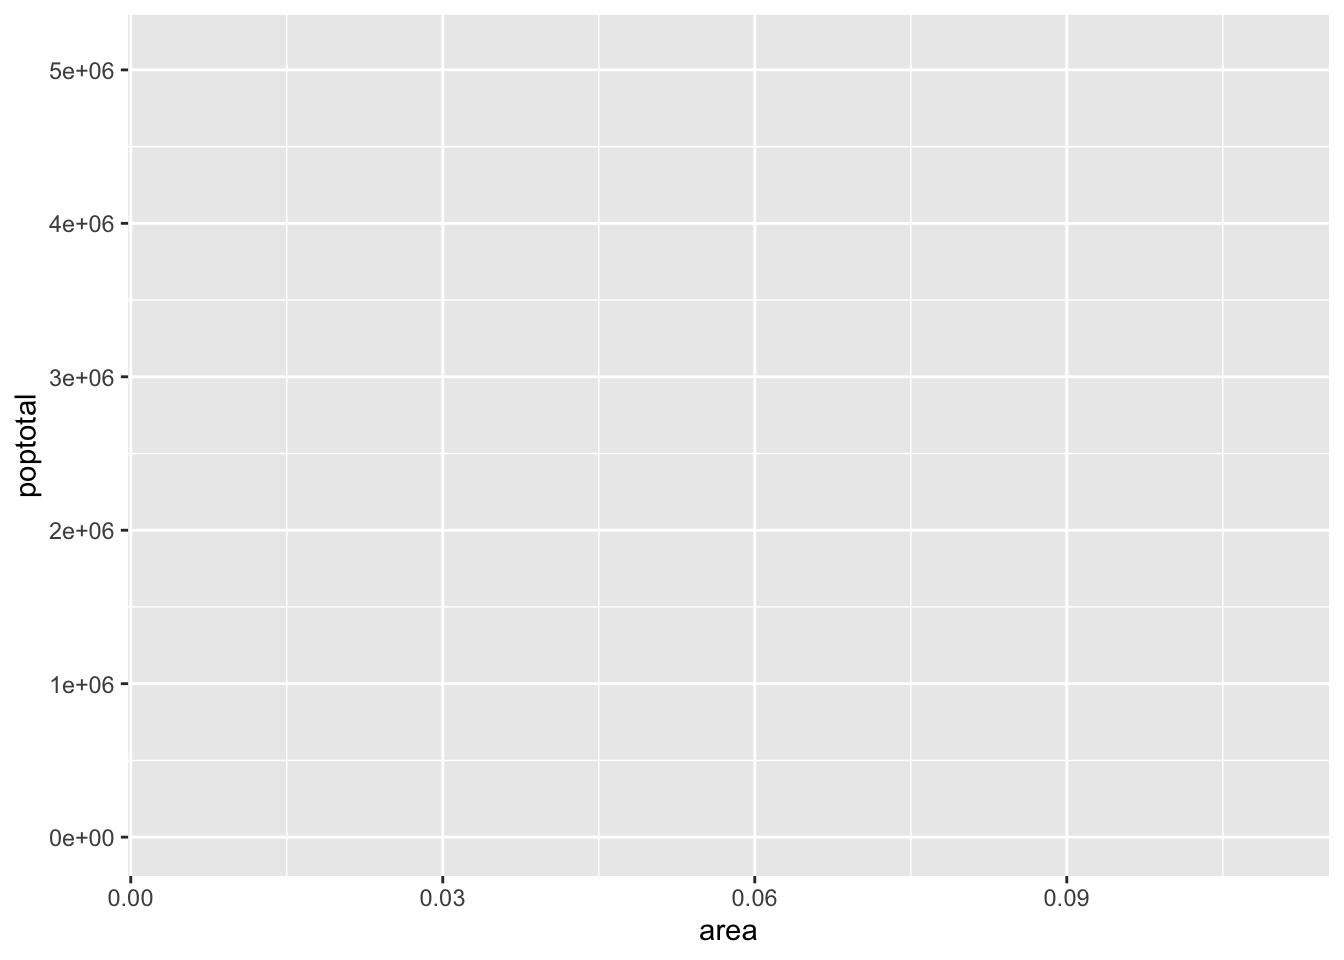
\includegraphics{t4ds/week2_files/figure-pdf/unnamed-chunk-6-1.pdf}

}

\end{figure}

What we see here is a blank ggplot! ggplot does not plot by default a
scatter or a line chart! We would need to decide next what should we
plot! Let's make a scatter plot.

\begin{Shaded}
\begin{Highlighting}[]
\FunctionTok{ggplot}\NormalTok{(midwest,}\FunctionTok{aes}\NormalTok{(}\AttributeTok{x=}\NormalTok{area,}\AttributeTok{y=}\NormalTok{poptotal)) }\SpecialCharTok{+} 
  \FunctionTok{geom\_point}\NormalTok{()}
\end{Highlighting}
\end{Shaded}

\begin{figure}[H]

{\centering 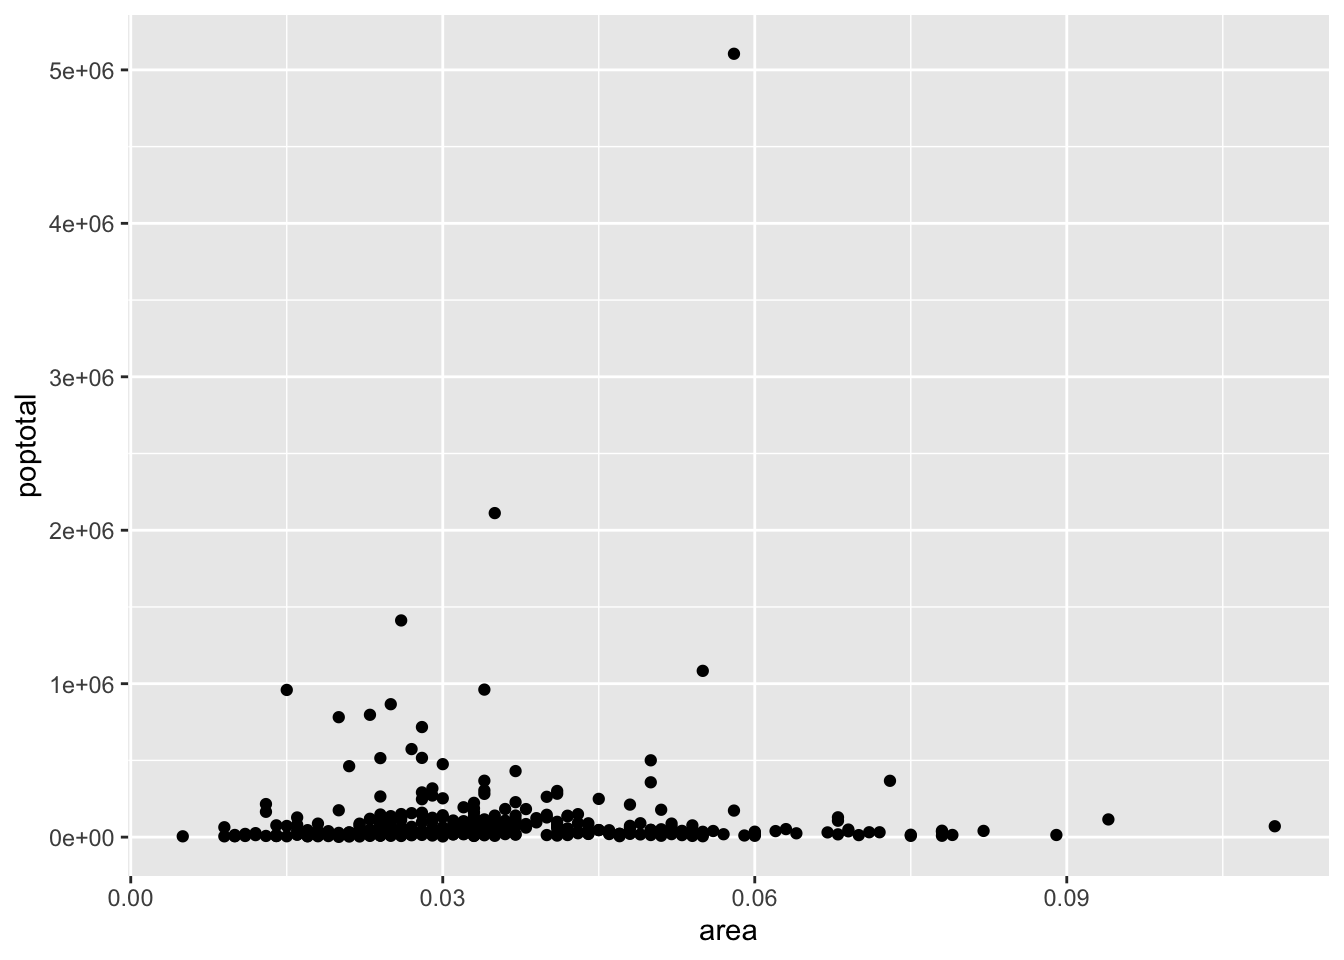
\includegraphics{t4ds/week2_files/figure-pdf/unnamed-chunk-7-1.pdf}

}

\end{figure}

Yaay! we did it. Next, let's add a linear regression model:
\(poptotal = \beta_0 + \beta_1 area\).

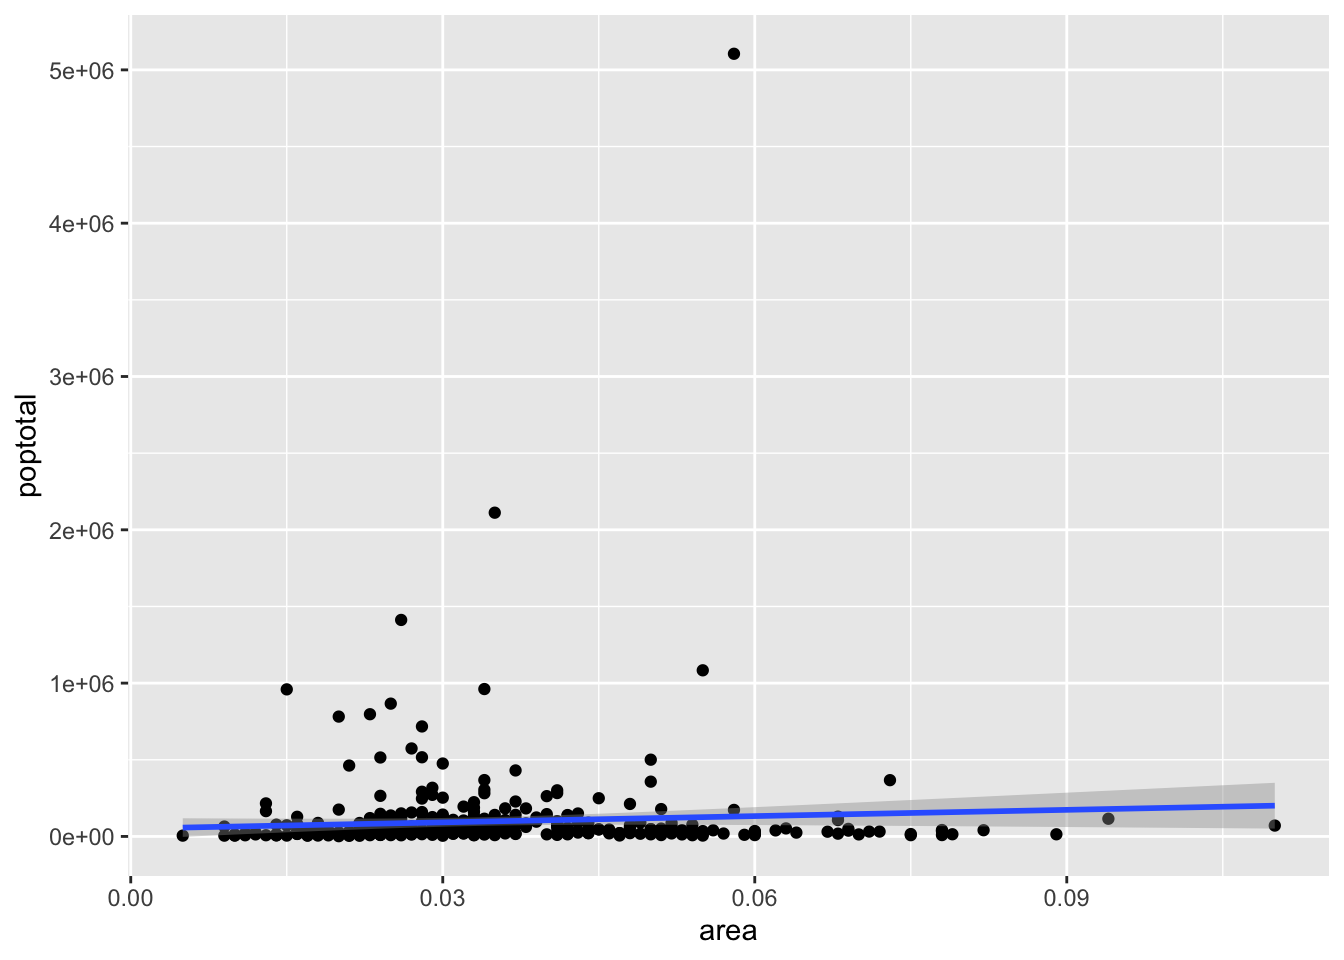
\includegraphics{t4ds/week2_files/figure-pdf/unnamed-chunk-8-1.pdf}

To control \emph{x} and \emph{y} axis limits, we can use \texttt{xlim()}
and \texttt{ylim()} as follows:

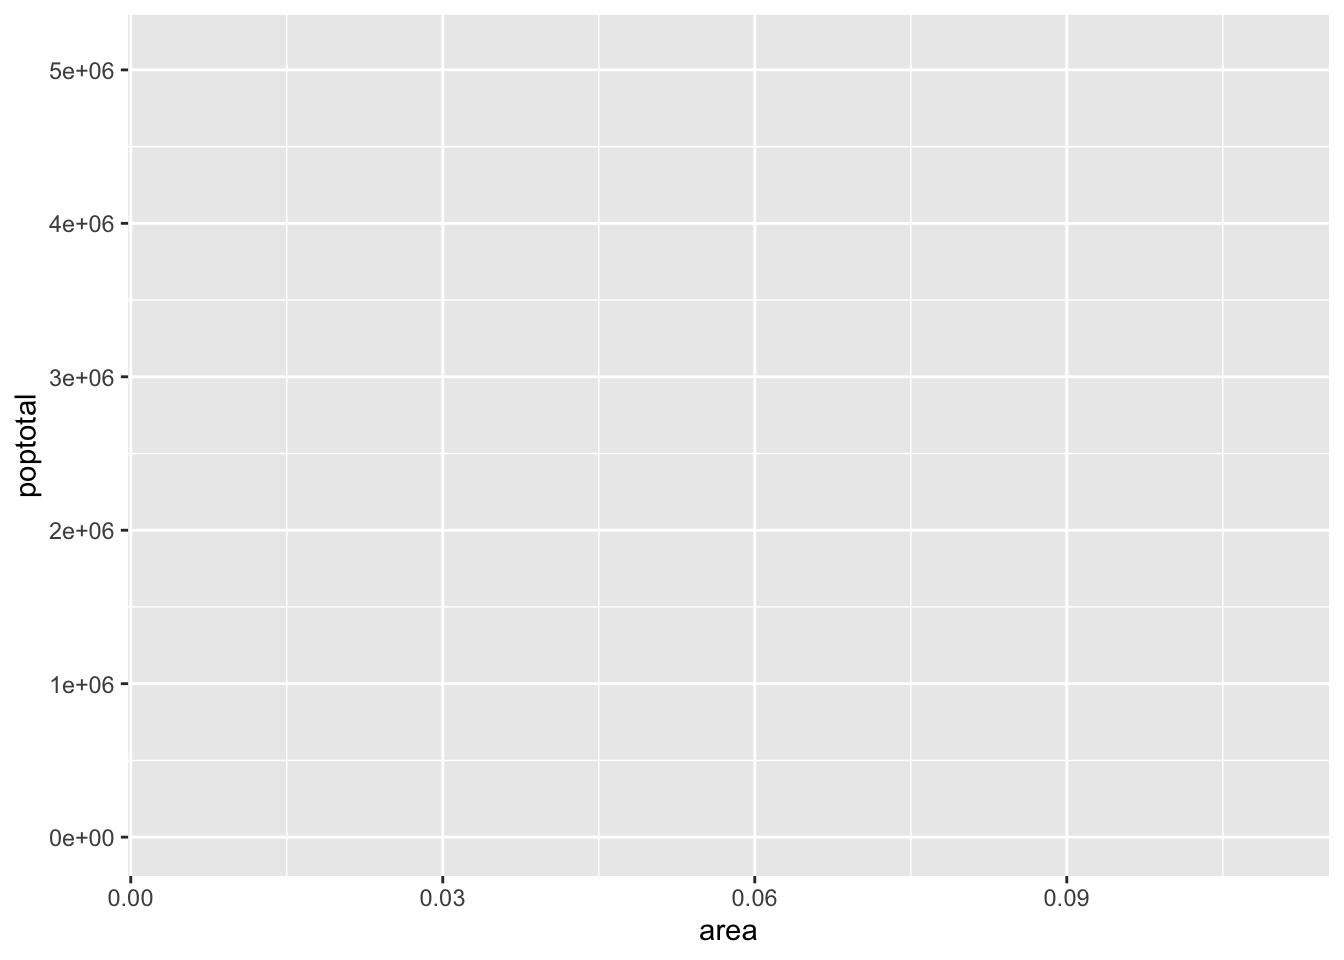
\includegraphics{t4ds/week2_files/figure-pdf/unnamed-chunk-9-1.pdf}

Notice that the line we obtain here is different from the line from the
first fit (all data included). This happens because ggplot will refit
the model \texttt{lm()} to data without the observations that are
outside the ranges. This is useful if we want to examine changes in the
model line when extreme values (or outliers) are removed.

We can also keep the model as the original plot and zoom in using:

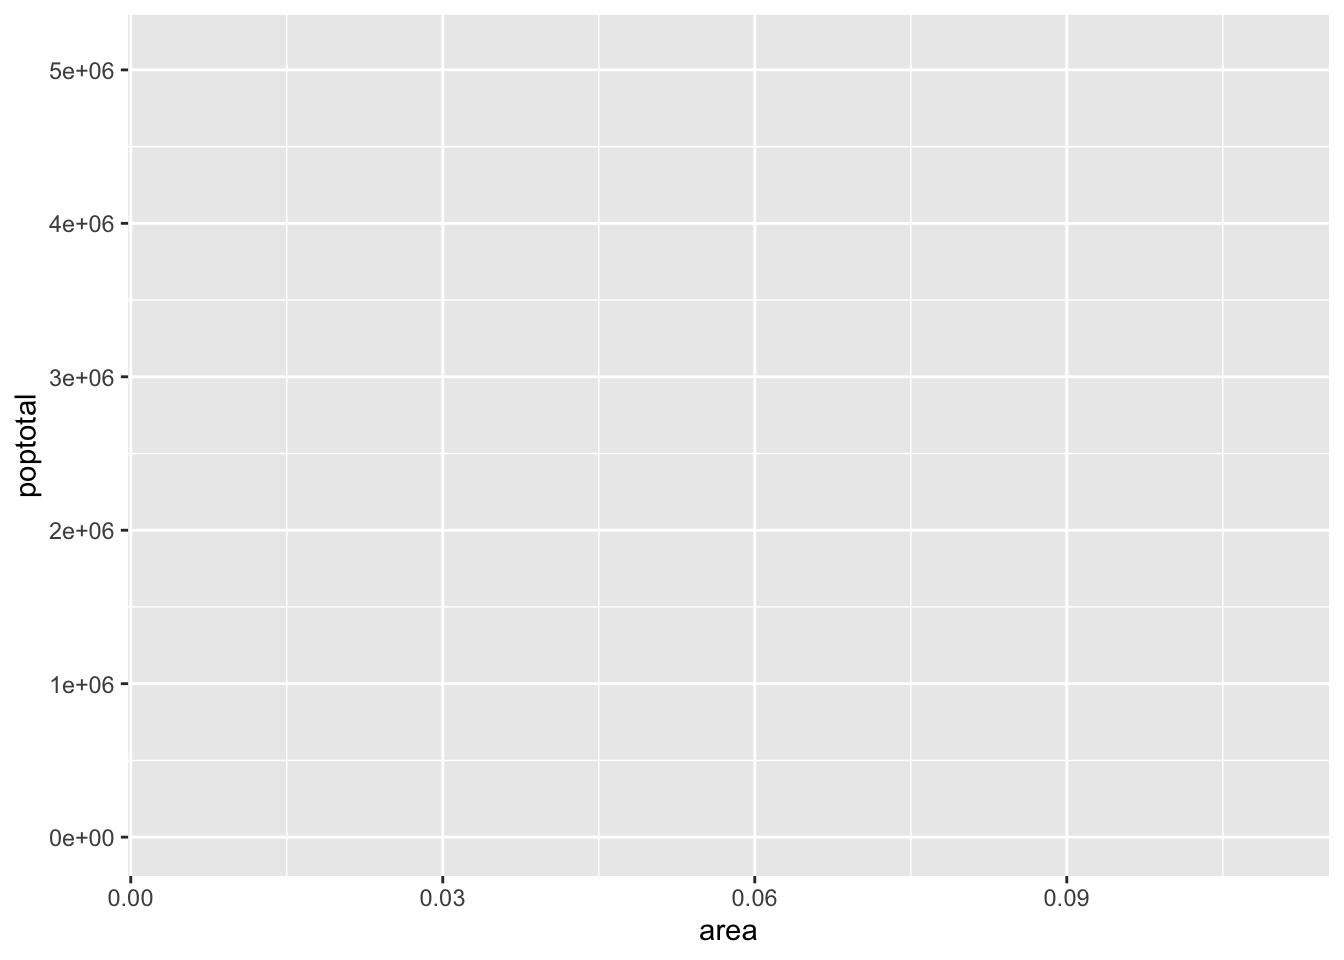
\includegraphics{t4ds/week2_files/figure-pdf/unnamed-chunk-10-1.pdf}

Let's Add some fancy options:

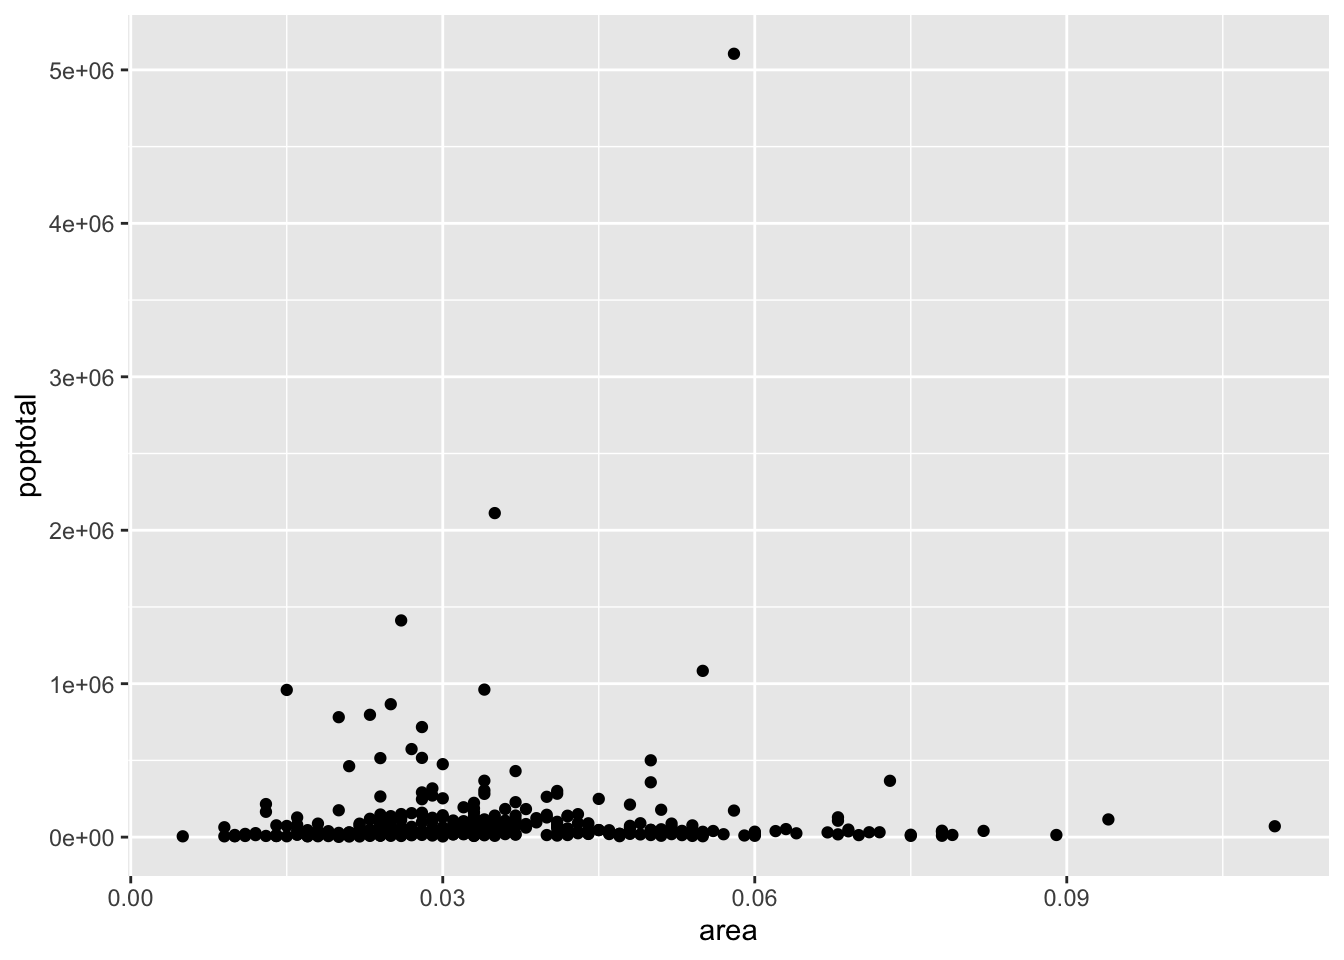
\includegraphics{t4ds/week2_files/figure-pdf/unnamed-chunk-11-1.pdf}

Wow! What about adding a new variable to the plot! For example, adding
\texttt{state} variable. Let's change the color to match the
\texttt{state} where a data point belongs to; \texttt{state} is a
variable in the \texttt{midwest} dataset.

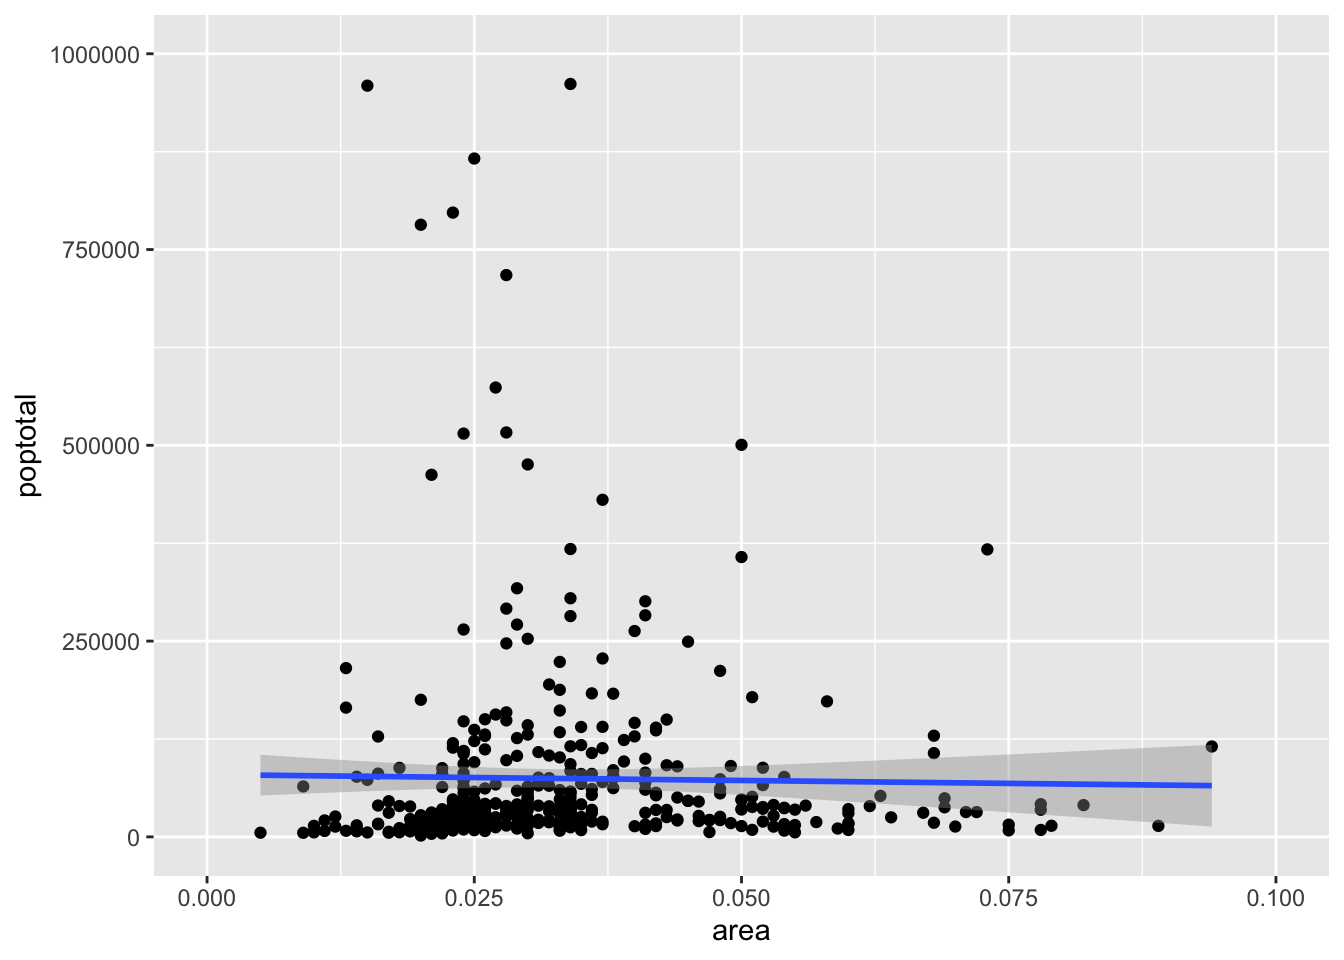
\includegraphics{t4ds/week2_files/figure-pdf/unnamed-chunk-12-1.pdf}

\hypertarget{and-more}{%
\section*{And more\ldots{}}\label{and-more}}
\addcontentsline{toc}{section}{And more\ldots{}}

\markright{And more\ldots{}}

Lessons of this week provide more about \texttt{tidyverse}. The
following will be covered more in details:

\begin{itemize}
\tightlist
\item
  Data manipulation (\texttt{filter}, \texttt{select}, \texttt{mutate},
  \texttt{arrange}, \texttt{summarize}, and etc.)
\item
  \texttt{ggplot2} package for data visualization.
\item
  An extended example
\end{itemize}

🛎 🎙️ Recordings on Canvas will cover more details and examples! Have fun
learning and coding 😃! Let me know how I can help!

\hypertarget{assignment---r-tidyverse}{%
\section*{📚 👈 Assignment - R
Tidyverse}\label{assignment---r-tidyverse}}
\addcontentsline{toc}{section}{📚 👈 Assignment - R Tidyverse}

\markright{📚 👈 Assignment - R Tidyverse}

Instructions are posted on Canvas.

\hypertarget{sql-basics}{%
\chapter*{SQL Basics}\label{sql-basics}}
\addcontentsline{toc}{chapter}{SQL Basics}

\markboth{SQL Basics}{SQL Basics}

At the end of this week, you will be able to:

\begin{itemize}
\tightlist
\item
  Identify \emph{Structured Query Language} queries
\item
  Write your first SQL queries
\end{itemize}

Let's start with defining the basics.

\hypertarget{database}{%
\section*{Database}\label{database}}
\addcontentsline{toc}{section}{Database}

\markright{Database}

A \emph{database} is an organized collection of data stored and accessed
electronically from a computer system. A Database Management System
(DBMS) is a software that is used to manage databases.

\begin{figure}

{\centering 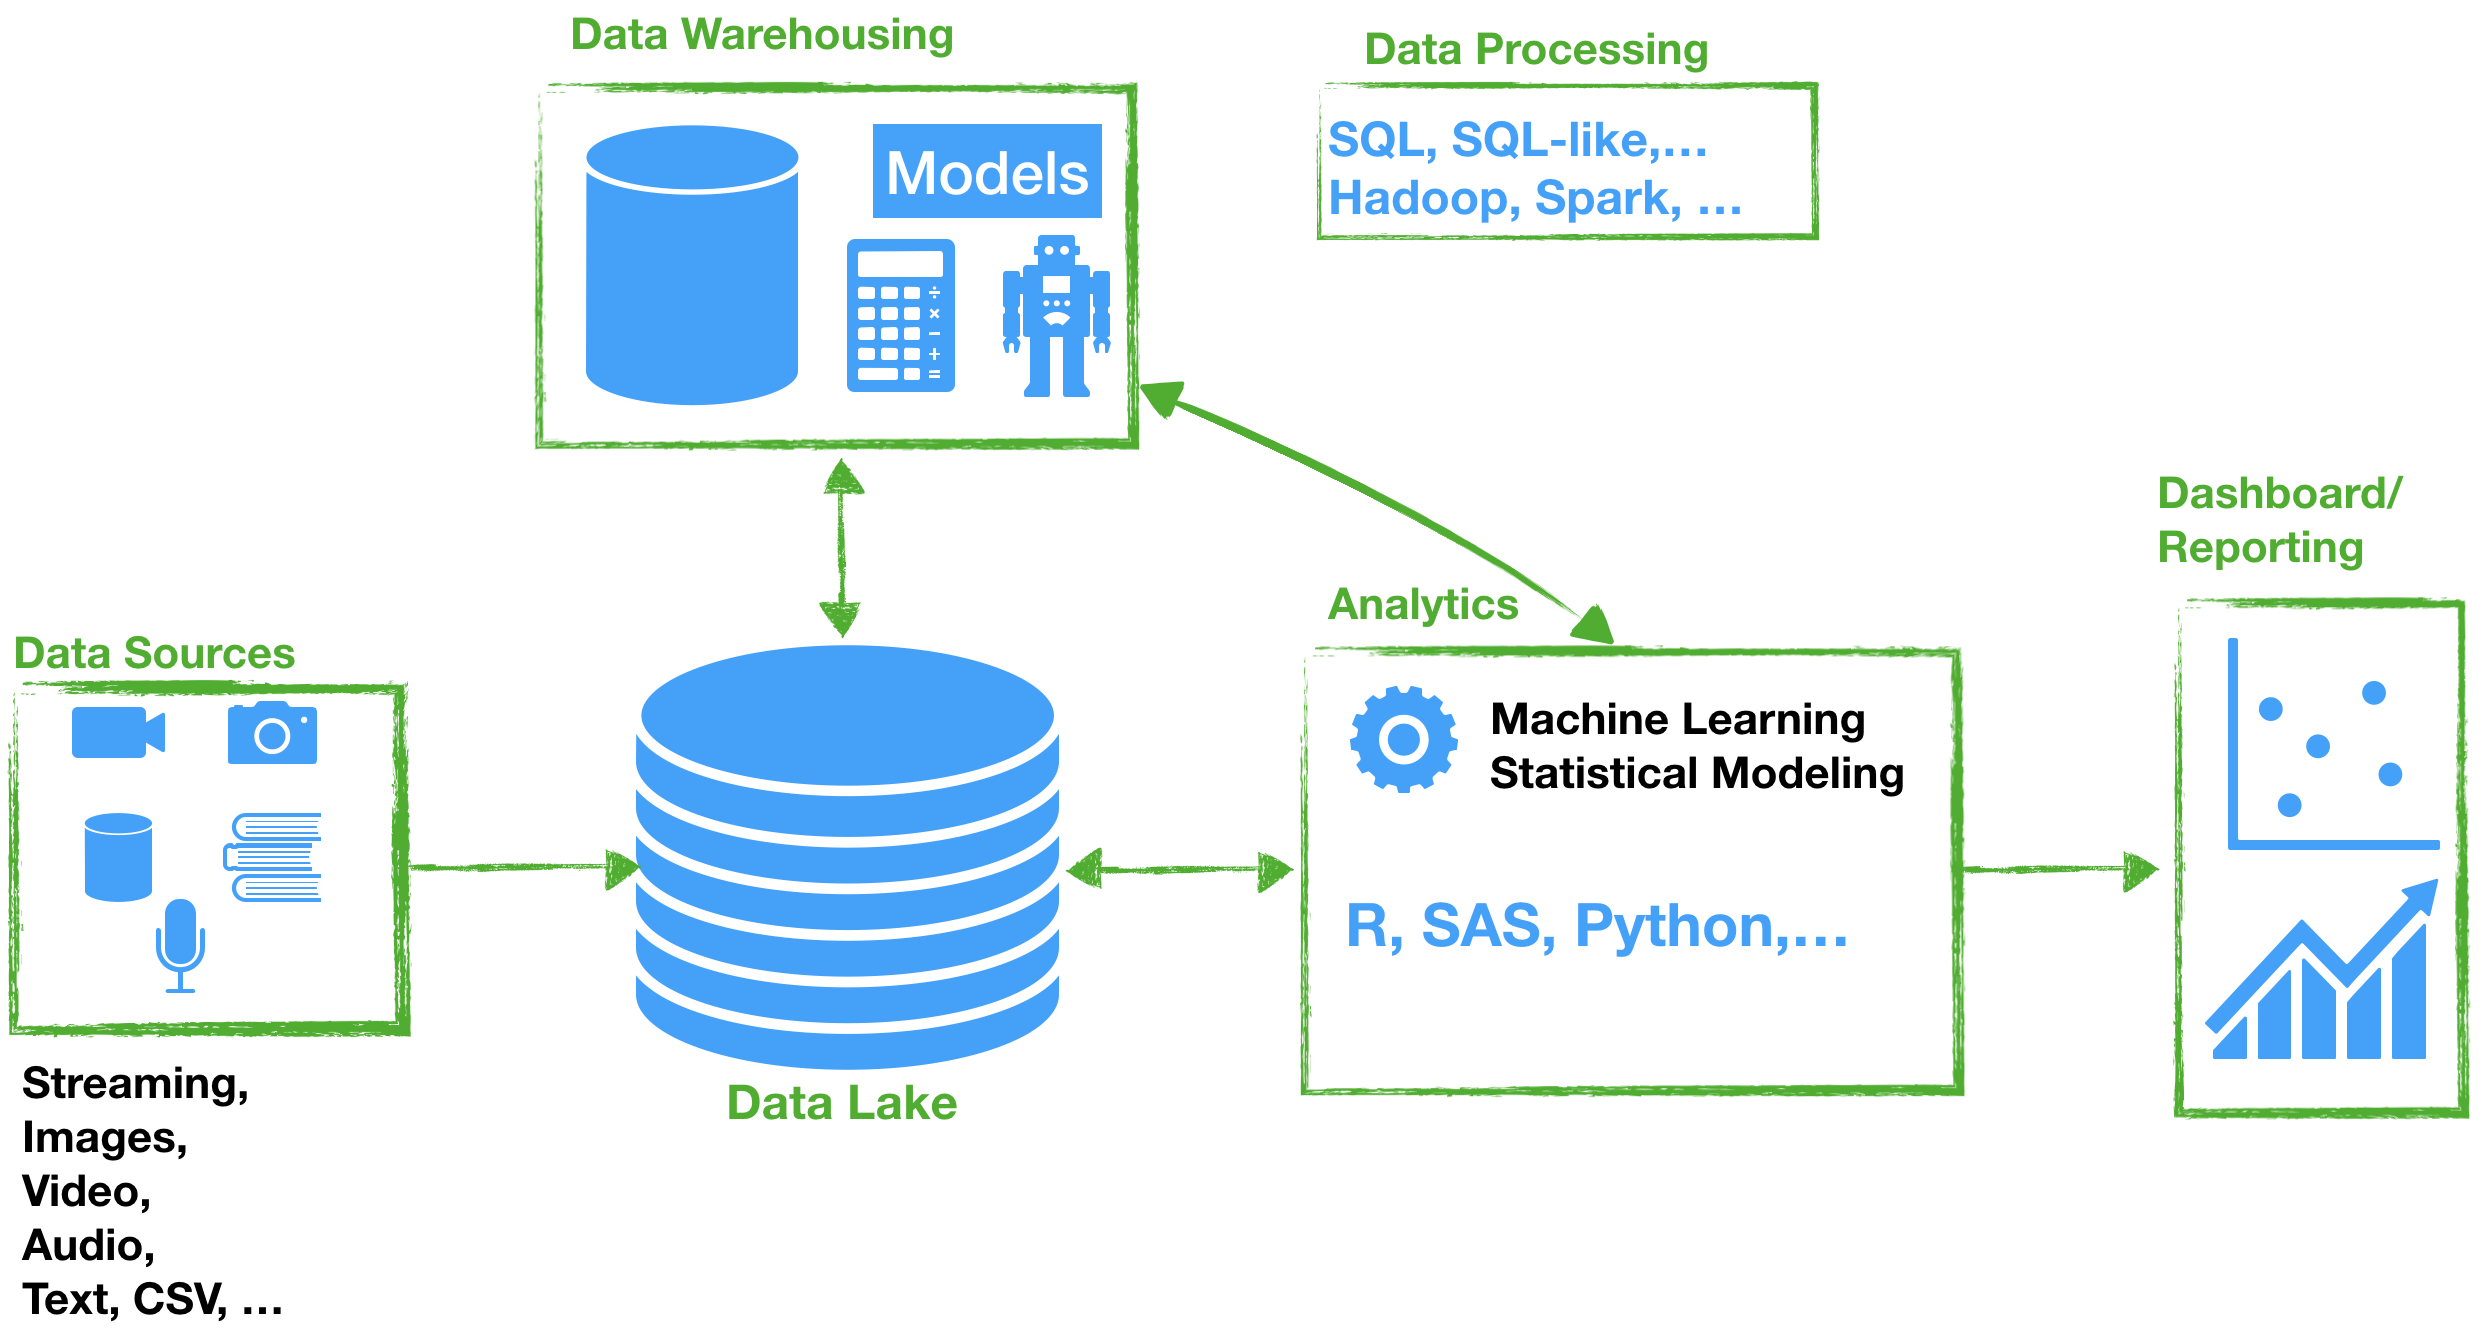
\includegraphics{img/DSWorkflow.png}

}

\caption{Data Science}

\end{figure}

In order to work with data that are stored in databases we need a
language. \emph{SQL} is a standard computer language for relational
database management systems (RDBMS). It is used for storing,
manipulating and retrieving data in databases.

\emph{SQL} has various dialects such as PL/SQL (Oracle), T-SQL
(Microsoft), and others.

In this course, we will use \textbf{SQL Server Management Studio} hosted
at UWF servers. We will use the fictional company
\href{https://docs.microsoft.com/en-us/previous-versions/sql/sql-server-2008/ms124623(v=sql.100)}{Adventure
Works data}.

Information about accessing the SQL Server is posted on Canvas.

\hypertarget{basic-concepts}{%
\subsection*{Basic concepts}\label{basic-concepts}}
\addcontentsline{toc}{subsection}{Basic concepts}

When dealing with databases we will need to know what is:

\begin{itemize}
\item
  \textbf{Entity}: is any thing the data represents in a database. For
  example, \texttt{Students}, \texttt{Employees}, \texttt{Schools},
  \texttt{Departments}, etc. There are given as tables.
\item
  \textbf{Data Type}: We need to pick a data type for each column when
  creating a table. There are common data types including
  \texttt{INTEGER}, \texttt{FLOAT}, \texttt{CURRENCY}, \texttt{DATE},
  \texttt{BOOLEAN}, and etc.
\item
  \textbf{Data Definition Language (DDL)}: DDL commands are used to
  create or modify database structures. \texttt{CREATE}, \texttt{ALTER},
  and \texttt{DROP} are examples of DDL commands.
\item
  \textbf{Data Manipulation Language (DML)}: DML commands are used to
  insert, retrieve, or modify data. \texttt{INSERT}, \texttt{DELETE},
  and \texttt{UPDATE} are examples of DML commands.
\item
  \textbf{Data Control Language (DCL)}: DCL commands are used to create
  rights and permission. \texttt{GRANT} and \texttt{REVOKE} are examples
  of DCL commands.
\item
  \textbf{Query}: Data scientists use a query to get data or information
  from database tables.
\end{itemize}

\hypertarget{data-language}{%
\section*{Data Language}\label{data-language}}
\addcontentsline{toc}{section}{Data Language}

\markright{Data Language}

Now that we have access to
\href{https://argoapps.uwf.edu/vpn/index.html}{SQL server system}, we
are ready to manipulate some data and execute \emph{SQL} queries.
\emph{SQL} statements are divided into \textbf{3 categories}: DDL, DML,
and DCL. We can execute \emph{SQL} queries using \emph{SQL Command} or
using Graphic User Interface (\emph{GUI}). We shall present next common
statements for DDL and DML.

\hypertarget{data-definition-language-ddl}{%
\subsection*{Data Definition Language
(DDL)}\label{data-definition-language-ddl}}
\addcontentsline{toc}{subsection}{Data Definition Language (DDL)}

The DDL statements are used to create databases and tables. Here is a
list of some of the statements:

\begin{itemize}
\tightlist
\item
  SQL commands to create a \emph{database}:
\end{itemize}

\textbf{\texttt{CREATE\ DATABASE}}\texttt{database\_name;}

\begin{itemize}
\tightlist
\item
  SQL commands to delete a \emph{database}:
\end{itemize}

\textbf{\texttt{DROP\ DATABASE}}\texttt{database\_name;}

⚠️ be very careful to drop databases or tables!

\begin{itemize}
\tightlist
\item
  SQL commands to create a \emph{Table}:
\end{itemize}

\textbf{\texttt{CREATE\ TABLE}}\texttt{table\_name;}

\begin{itemize}
\tightlist
\item
  SQL commands to create a \emph{Table} from an existing table:
\end{itemize}

\textbf{\texttt{SELECT...\ INTO}}\texttt{table\_name}
\textbf{\texttt{FROM}} \texttt{Orginal\_table}

\begin{itemize}
\tightlist
\item
  SQL commands to drop a \emph{Table}:
\end{itemize}

\textbf{\texttt{DROP\ TABLE}}\texttt{table\_name;}

\begin{itemize}
\tightlist
\item
  SQL commands to truncating (remove all records from a table) a
  \emph{Table}:
\end{itemize}

\textbf{\texttt{TRUNCATE\ TABLE}}\texttt{table\_name;}

\hypertarget{data-maniplulation-language-dml}{%
\subsection*{\texorpdfstring{\textbf{Data Maniplulation Language
(DML)}}{Data Maniplulation Language (DML)}}\label{data-maniplulation-language-dml}}
\addcontentsline{toc}{subsection}{\textbf{Data Maniplulation Language
(DML)}}

The DDL statements are used to insert data, update records, and delete
records. Data Manipulation Language is used to manipulate data. Here is
a list of the main statements:

\begin{itemize}
\tightlist
\item
  SQL commands to insert one or more records into a \emph{Table}:
\end{itemize}

\textbf{\texttt{INSERT\ INTO}}\texttt{table\_name(col1,col2,...)}
\textbf{\texttt{VALUES}}\texttt{(exp1,exp2,...);}

\textbf{\texttt{INSERT\ INTO}}\texttt{table\_name}
\textbf{\texttt{VALUES}}\texttt{(exp1,exp2,...);}

⚠️ Make sure you insert data in the same order as that in the table for
the second syntax.

\begin{itemize}
\tightlist
\item
  SQL commands to select records from one or more \emph{Tables}:
\end{itemize}

\textbf{\texttt{SELECT}}\texttt{column(s)}
\textbf{\texttt{FROM}}\texttt{tables}
\textbf{\texttt{WHERE}}\texttt{conditions} (optional)
\textbf{\texttt{ORDER\ BY}} \texttt{column(s)ASC\ \textbar{}\ DESC;}
(optional)

\begin{itemize}
\tightlist
\item
  \texttt{DISTINCT} clause to eliminate duplicates:
\end{itemize}

\textbf{\texttt{SELECT\ DISTINCT}}\texttt{column\_name}
\textbf{\texttt{FROM}}\texttt{table\_name;}

\begin{itemize}
\tightlist
\item
  \texttt{WHERE} clause to filter if the condition is true:
\end{itemize}

\textbf{\texttt{SELECT}}\texttt{column(s)}
\textbf{\texttt{FROM}}\texttt{table\_name}
\textbf{\texttt{WHERE}}\texttt{conditions;}

\begin{itemize}
\tightlist
\item
  Arithmetic operators
\end{itemize}

\textbf{\texttt{SELECT}}\texttt{column\_name1,\ column\_name2,\ column\_name2*2\ AS\ \textquotesingle{}twicecolumn2\textquotesingle{}}
\textbf{\texttt{FROM}}\texttt{table\_name;}

Basic \textbf{arithmetic} operators include:
\textbf{\texttt{\%}}\texttt{modulo},
\textbf{\texttt{/}}\texttt{division},
\textbf{\texttt{*}}\texttt{multiplication},
\textbf{\texttt{+}}\texttt{addition}, and
\textbf{\texttt{-}}\texttt{substraction}.

Basic \textbf{comparison} operators include:
\textbf{\texttt{=}}\texttt{equal\ to},
\textbf{\texttt{\textless{}\textgreater{}}}\texttt{not\ equal\ to},
\textbf{\texttt{\textgreater{}}}\texttt{greater\ than},
\textbf{\texttt{\textgreater{}=}}\texttt{greater\ than\ equal\ to}, and
more.

Basic \textbf{condition} operators include:
\textbf{\texttt{AND}}\texttt{all\ conditions\ must\ be\ true\ to\ get\ true},
\textbf{\texttt{OR}}\texttt{Any\ one\ of\ the\ conditions\ must\ be\ true\ to\ get\ true},
\textbf{\texttt{IN}}\texttt{test\ if\ an\ expression\ matches\ any\ value\ in\ a\ list\ of\ VALUES},
\textbf{\texttt{BETWEEN}}\texttt{check\ if\ an\ experession\ is\ within\ a\ range\ of\ VALUES},
and more.

\begin{itemize}
\tightlist
\item
  \texttt{ORDER\ BY} clause to sort the records:
\end{itemize}

\textbf{\texttt{SELECT}}\texttt{column(s)}
\textbf{\texttt{FROM}}\texttt{table\_name}
\textbf{\texttt{WHERE}}\texttt{conditions}
\textbf{\texttt{ORDER\ BY}}\texttt{expression\ (by\ default\ ASC);}

\begin{itemize}
\tightlist
\item
  \texttt{UPDATE} statement to update records:
\end{itemize}

\textbf{\texttt{UPDATE}}\texttt{table}
\textbf{\texttt{SET}}\texttt{col1\ =\ value1,\ col2\ =\ value2,\ ...}
\textbf{\texttt{WHERE}}\texttt{conditions\ {[}optional{]};}

\begin{itemize}
\tightlist
\item
  \texttt{DELETE} statement to delete records:
\end{itemize}

\textbf{\texttt{DELETE\ FROM}}\texttt{table}
\textbf{\texttt{WHERE}}\texttt{conditions\ {[}optional{]};}

\hypertarget{functions-and-group-by}{%
\section*{Functions and GROUP BY}\label{functions-and-group-by}}
\addcontentsline{toc}{section}{Functions and GROUP BY}

\markright{Functions and GROUP BY}

Often you will be asked to answer questions that involve writing queries
for summaries using aggregate function and \texttt{GROUP\ BY} clause.

\begin{itemize}
\tightlist
\item
  \textbf{SQL commands for Aggregate statements}:
\end{itemize}

\textbf{\texttt{SELECT\ Aggregate\ Function}}\texttt{column\_name}
\textbf{\texttt{FROM}}\texttt{table\_name;}

Below are the main aggregate functions:

\begin{longtable}[]{@{}
  >{\raggedright\arraybackslash}p{(\columnwidth - 2\tabcolsep) * \real{0.1831}}
  >{\raggedright\arraybackslash}p{(\columnwidth - 2\tabcolsep) * \real{0.8169}}@{}}
\toprule\noalign{}
\begin{minipage}[b]{\linewidth}\raggedright
Function
\end{minipage} & \begin{minipage}[b]{\linewidth}\raggedright
Action
\end{minipage} \\
\midrule\noalign{}
\endhead
\bottomrule\noalign{}
\endlastfoot
\texttt{AVG()} & average values \\
\texttt{COUNT()} & count the number of rows in a table \\
\texttt{MAX()} & select the highest value select the latest date select
the last record for a character \\
\texttt{MIN()} & select the lowest value select the earliest date select
the first record for a character \\
\texttt{SUM()} & return the total for a numeric column \\
\texttt{ROUND()} & round a number to specific decimal \\
& \\
\end{longtable}

In addition to aggregate functions, there are other type of functions:

-\emph{The \textbf{number} functions} take a numeric as an input and
return a numeric value. The common number functions include
\texttt{CEILING()}, \texttt{FLOOR()}, \texttt{\%}, \texttt{POWER(m,n)}
{[}\(m^n\){]}, \texttt{SQRT()}, and \texttt{ROUND()}.

-\emph{The \textbf{string} functions}. The common string functions
include \texttt{CONCAT()}, \texttt{LEFT()}, \texttt{LEN()},
\texttt{LOWER()}, \texttt{REPLACE()}, \texttt{RIGHT()},
\texttt{UPPER()}, and \texttt{SUBSTRING()}.

-\emph{The \textbf{Date and Time} functions}. The common date and time
functions include \texttt{CURRENT\_TIMESTAMP()}, \texttt{DATEADD()},
\texttt{DATEPART()}, \texttt{GETDATE()}, \texttt{DATEDIFF()}, and
\texttt{SYSDATETIME()}.

-\emph{The \textbf{Conversion} functions}. The common conversion
functions include \texttt{CAST()} and \texttt{CONVERT()}.

\begin{itemize}
\tightlist
\item
  \textbf{GROUP BY and HAVING Clause}:
\end{itemize}

The GROUP BY statement is used to group data from a column. HAVING
clause is used with a GROUP BY to add conditions on groups.

\textbf{\texttt{SELECT\ Aggregate\ Function}}\texttt{column\_name}
\textbf{\texttt{FROM}}\texttt{table\_name}
\textbf{\texttt{WHERE}}\texttt{conditions\ -\ optional}
\textbf{\texttt{GROUP\ BY}}\texttt{column\_name}
\textbf{\texttt{HAVING}}\texttt{conditions\ -\ optional}
\textbf{\texttt{ORDER\ BY}}\texttt{column(s)\ {[}ASC\ \textbar{}\ DESC{]}\ -\ optional;}

🛎 🎙️ Recordings on Canvas will cover more details and examples! Have fun
learning and coding 😃! Let me know how I can help!

\hypertarget{assignments---sql-basics}{%
\section*{📚 👈 Assignments - SQL
basics}\label{assignments---sql-basics}}
\addcontentsline{toc}{section}{📚 👈 Assignments - SQL basics}

\markright{📚 👈 Assignments - SQL basics}

Instructions are posted on Canvas.

\hypertarget{advanced-sql}{%
\chapter*{Advanced SQL}\label{advanced-sql}}
\addcontentsline{toc}{chapter}{Advanced SQL}

\markboth{Advanced SQL}{Advanced SQL}

At the end of this week, you will be able to:

\begin{itemize}
\tightlist
\item
  Practice with advanced \emph{SQL}
\item
  Evaluate \texttt{UNION}, \texttt{Subqueries}, \texttt{EXCEPT}, and
  other \emph{SQL} commands.
\item
  Apply \texttt{JOINS}
\end{itemize}

\hypertarget{advanced-sql-commands}{%
\section*{Advanced SQL commands}\label{advanced-sql-commands}}
\addcontentsline{toc}{section}{Advanced SQL commands}

\markright{Advanced SQL commands}

SQL commands to return all rows from two tables:

\texttt{SELECT\ column(s)} \texttt{FROM\ table1}
\textbf{\texttt{UNION\ ALL}} \texttt{SELECT\ column(s)}
\texttt{FROM\ table2;}

SQL commands to return only rows that exist in both tables:

\texttt{SELECT\ column(s)} \texttt{FROM\ table1}
\textbf{\texttt{INTERSECT}} \texttt{SELECT\ column(s)}
\texttt{FROM\ table2;}

SQL commands to return all rows in the first SELECT but excludes those
by the second SELECT:

\texttt{SELECT\ col1,col2,...} \texttt{FROM\ table1}
\textbf{\texttt{EXCEPT}} \texttt{SELECT\ col1,col2,...}
\texttt{FROM\ table2;}

SQL command to specify the number of records to return:

\texttt{SELECTTOPnumber\ \textbar{}\ percent\ column\_names(s)\ \textless{}br/\textgreater{}}FROM
table\_name;`

\hypertarget{subqueries}{%
\section*{Subqueries}\label{subqueries}}
\addcontentsline{toc}{section}{Subqueries}

\markright{Subqueries}

A \emph{Subquery} is a SQL query nested inside a SQL query. Very useful
to create a virtual table usable by the main query.

\texttt{SELECT\ column(s)} \texttt{FROM\ table1}
\texttt{WHERE\ value\ IN} (\textbf{\texttt{SELECT\ column\_name}}
\textbf{\texttt{FROM\ tables2}} \textbf{\texttt{WHERE\ conditions);}}

\hypertarget{joins}{%
\section*{Joins}\label{joins}}
\addcontentsline{toc}{section}{Joins}

\markright{Joins}

Relational databases are defined with tables or entities such
\emph{Employee} and \emph{Department}. To create a link between the two
tables a column is defined as \emph{Department\_ID} in both tables. Now,
if you would like to extract employee names and departments names you
need to SQL JOIN.

There are four main type of joins:

\begin{longtable}[]{@{}
  >{\raggedright\arraybackslash}p{(\columnwidth - 2\tabcolsep) * \real{0.1456}}
  >{\raggedright\arraybackslash}p{(\columnwidth - 2\tabcolsep) * \real{0.8544}}@{}}
\toprule\noalign{}
\begin{minipage}[b]{\linewidth}\raggedright
JOIN
\end{minipage} & \begin{minipage}[b]{\linewidth}\raggedright
Action
\end{minipage} \\
\midrule\noalign{}
\endhead
\bottomrule\noalign{}
\endlastfoot
\texttt{INNER\ JOIN} & return records that have matching values in both
tables \\
\texttt{LEFT\ JOIN} & return all records from table1 (\textbf{LEFT}
table1) and the matched records from table2 \\
\texttt{RIGHT\ JOIN} & return all records from table2 (\textbf{RIGHT}
table1) and the matched records from table1. \\
\texttt{FULL\ JOIN()} & return all rows from both tables \\
& \\
\end{longtable}

Syntax:

\texttt{SELECT\ table1.col\_name,\ table2.col\_name}
\texttt{FROM\ table1} \textbf{\texttt{INNER\ JOIN}} \texttt{table2ON}
\texttt{table1.col\_name\ =\ table2.col\_name;}

OR

\texttt{SELECT\ table1.col\_name,\ table2.col\_name}
\texttt{FROM\ table1} \textbf{\texttt{LEFT\ JOIN}} \texttt{table2ON}
\texttt{table1.col\_name\ =\ table2.col\_name;}

OR

\texttt{SELECT\ table1.col\_name,\ table2.col\_name}
\texttt{FROM\ table1} \textbf{\texttt{RIGHT\ JOIN}} \texttt{table2ON}
\texttt{table1.col\_name\ =\ table2.col\_name;}

OR

\texttt{SELECT\ table1.col\_name,\ table2.col\_name}
\texttt{FROM\ table1} \textbf{\texttt{FULL\ JOIN}} \texttt{table2ON}
\texttt{table1.col\_name\ =\ table2.col\_name;}

🛎 🎙️ Recordings on Canvas will cover more details and examples! Have fun
learning and coding 😃! Let me know how I can help!

\hypertarget{assignments---advanced-sql}{%
\section*{📚 👈 Assignments - Advanced
SQL}\label{assignments---advanced-sql}}
\addcontentsline{toc}{section}{📚 👈 Assignments - Advanced SQL}

\markright{📚 👈 Assignments - Advanced SQL}

Instructions are posted on Canvas.

\hypertarget{python-basics---numpy-and-pandas}{%
\chapter*{Python Basics - NumPy and
Pandas}\label{python-basics---numpy-and-pandas}}
\addcontentsline{toc}{chapter}{Python Basics - NumPy and Pandas}

\markboth{Python Basics - NumPy and Pandas}{Python Basics - NumPy and
Pandas}

At the end of this week, you will be able to:

\begin{itemize}
\tightlist
\item
  Practice with \emph{Python} Basics
\item
  Practice using \textbf{NumPy} and \textbf{Pandas} libraries
\item
  Write your first \emph{Python} script!
\end{itemize}

\hypertarget{references}{%
\section*{References}\label{references}}
\addcontentsline{toc}{section}{References}

\markright{References}

\begin{itemize}
\tightlist
\item
  \emph{Python Data Science Handbook}
  (\protect\hyperlink{ref-Jake2016python}{VanderPlas 2016}).
  \href{https://jakevdp.github.io/PythonDataScienceHandbook/00.00-preface.html}{Free
  access}
\item
  \emph{Think Python} (\protect\hyperlink{ref-Allenpython}{Downey
  2015}).
  \href{https://greenteapress.com/thinkpython2/thinkpython2.pdf}{Free
  access}
\item
  \emph{Data Science and Analytics with Python}
  (\protect\hyperlink{ref-rogel2018data}{Rogel-Salazar 2018})
\end{itemize}

\hypertarget{introduction-to-python}{%
\section*{Introduction to Python}\label{introduction-to-python}}
\addcontentsline{toc}{section}{Introduction to Python}

\markright{Introduction to Python}

\textbf{Python} has emerged over the last recent years as one of the
most used tools for data science projects. It is known for code
readability and interactive features. Similar to \textbf{R},
\textbf{Python} is supported by a \href{https://pypi.org/}{large number
of packages} that extend its features and functions. Common packages
are, to name few:

\begin{itemize}
\tightlist
\item
  \href{https://numpy.org/doc/stable/}{NumPy}: provides functions for
  manipulating arrays
\item
  \href{https://pandas.pydata.org/docs/}{Pandas}: provides functions for
  manipulating data frames
\item
  \href{https://matplotlib.org/stable/tutorials/index.html}{Matplotlib}:
  provides functions for visualizations and plotting
\item
  \href{https://www.statsmodels.org/stable/gettingstarted.html}{Statsmodels}:
  provides functions for statistical models
\item
  \href{https://scikit-learn.org/stable/}{Scikit-learn}: provides
  functions for machine learning algorithms
\end{itemize}

\hypertarget{getting-started-with-python}{%
\section*{Getting started with
Python}\label{getting-started-with-python}}
\addcontentsline{toc}{section}{Getting started with Python}

\markright{Getting started with Python}

We will use RStudio IDE to run Python but, there are other IDEs that you
may want to check for your information such as
\href{https://www.jetbrains.com/pycharm/}{Pycharm},
\href{https://jupyter.org/}{Jupyter}, and others. We will be using
\texttt{Python\ 3}. We will see that there are multiple similarities
between R and Python.

\begin{quote}
\textbf{Indentation} refers to the spaces at the beginning of a code
line. The indentation in Python is very important.
\end{quote}

Recordings of this week provide lessons about the following concepts:

\hypertarget{python-basics}{%
\section*{Python Basics}\label{python-basics}}
\addcontentsline{toc}{section}{Python Basics}

\markright{Python Basics}

\begin{itemize}
\tightlist
\item
  Python Variables:
\end{itemize}

\begin{Shaded}
\begin{Highlighting}[]
\CommentTok{\# This is Python Code}
\BuiltInTok{print}\NormalTok{(}\StringTok{"Hello World!"}\NormalTok{)}
\end{Highlighting}
\end{Shaded}

\begin{verbatim}
Hello World!
\end{verbatim}

You can name a variable following these rules:

\begin{itemize}
\tightlist
\item
  One word
\item
  Use only letters, numbers, and the underscore (\_) character
\item
  Can't begin with a number
\item
  Python is case-sensitive
\end{itemize}

\begin{Shaded}
\begin{Highlighting}[]
\NormalTok{x }\OperatorTok{=} \StringTok{"HeyHey"}
\NormalTok{y }\OperatorTok{=} \DecValTok{40}
\NormalTok{x}
\NormalTok{y}
\NormalTok{x, y }\OperatorTok{=} \StringTok{"Hey"}\NormalTok{, }\DecValTok{45} \CommentTok{\# Assign values to multiple variables}
\BuiltInTok{print}\NormalTok{(x)}
\BuiltInTok{print}\NormalTok{(y)}
\NormalTok{ranks }\OperatorTok{=}\NormalTok{ [}\StringTok{"first"}\NormalTok{,}\StringTok{"second"}\NormalTok{,}\StringTok{"third"}\NormalTok{] }\CommentTok{\# list}
\NormalTok{x, y, z }\OperatorTok{=}\NormalTok{ ranks}
\BuiltInTok{print}\NormalTok{(ranks)}
\NormalTok{x}
\NormalTok{y}
\NormalTok{z}

\KeywordTok{def}\NormalTok{ myf():}
\NormalTok{  x}\OperatorTok{=}\StringTok{"Hello"}
  \BuiltInTok{print}\NormalTok{(x)}
  
\NormalTok{myf()}

\KeywordTok{def}\NormalTok{ myf():}
  \KeywordTok{global}\NormalTok{ x }\CommentTok{\# x to be global {-} outside the function}
\NormalTok{  x}\OperatorTok{=}\StringTok{"Hello"}
  \BuiltInTok{print}\NormalTok{(x)}
  
\NormalTok{myf()}
\end{Highlighting}
\end{Shaded}

\begin{verbatim}
Hey
45
['first', 'second', 'third']
Hello
Hello
\end{verbatim}

Data Types:

\begin{Shaded}
\begin{Highlighting}[]
\NormalTok{x }\OperatorTok{=} \BuiltInTok{str}\NormalTok{(}\DecValTok{3}\NormalTok{)    }\CommentTok{\# x will be \textquotesingle{}3\textquotesingle{}}
\NormalTok{x }\OperatorTok{=} \BuiltInTok{int}\NormalTok{(}\DecValTok{3}\NormalTok{)    }\CommentTok{\# x will be 3}
\NormalTok{x }\OperatorTok{=} \BuiltInTok{float}\NormalTok{(}\DecValTok{3}\NormalTok{)  }\CommentTok{\# x is a float {-} 3.0}
\NormalTok{x }\OperatorTok{=} \OtherTok{1j}       \CommentTok{\# x is complex}
\NormalTok{x }\OperatorTok{=} \BuiltInTok{range}\NormalTok{(}\DecValTok{5}\NormalTok{,}\DecValTok{45}\NormalTok{)    }\CommentTok{\# x is a range type}
\NormalTok{x }\OperatorTok{=}\NormalTok{ [}\DecValTok{1}\NormalTok{,}\DecValTok{2}\NormalTok{,}\DecValTok{1}\NormalTok{,}\DecValTok{24}\NormalTok{,}\DecValTok{54}\NormalTok{,}\DecValTok{45}\NormalTok{,}\DecValTok{2}\NormalTok{,}\DecValTok{1}\NormalTok{]  }\CommentTok{\# x is a list}
\NormalTok{x }\OperatorTok{=}\NormalTok{ (}\DecValTok{1}\NormalTok{,}\DecValTok{2}\NormalTok{,}\DecValTok{1}\NormalTok{,}\DecValTok{24}\NormalTok{,}\DecValTok{54}\NormalTok{,}\DecValTok{45}\NormalTok{,}\DecValTok{2}\NormalTok{,}\DecValTok{1}\NormalTok{)  }\CommentTok{\# x is a tuple}
\NormalTok{x }\OperatorTok{=}\NormalTok{ \{}\StringTok{"name"}\NormalTok{ : }\StringTok{"Ach"}\NormalTok{, }\StringTok{"age"}\NormalTok{ : }\DecValTok{85}\NormalTok{\}  }\CommentTok{\# x is a dict (mapping)}
\end{Highlighting}
\end{Shaded}

Math operations:

\begin{Shaded}
\begin{Highlighting}[]
\DecValTok{5}\OperatorTok{+}\DecValTok{4}   \CommentTok{\# Addition}
\DecValTok{5}\OperatorTok{*}\DecValTok{4}   \CommentTok{\# Multiplication}
\DecValTok{5}\OperatorTok{**}\DecValTok{4}  \CommentTok{\# power / exponent}
\BuiltInTok{print}\NormalTok{(}\StringTok{"Hey"}\OperatorTok{*}\DecValTok{3}\NormalTok{) }\CommentTok{\# String operations}
\ImportTok{import}\NormalTok{ math }\ImportTok{as}\NormalTok{ mt }\CommentTok{\# More more math functions using package *math*}
\NormalTok{mt.cos(}\DecValTok{556}\NormalTok{) }\CommentTok{\# cosine function}
\ImportTok{import}\NormalTok{ random }\CommentTok{\# generate random numbers}
\BuiltInTok{print}\NormalTok{(random.randrange(}\DecValTok{1}\NormalTok{, }\DecValTok{10}\NormalTok{))}
\ImportTok{import}\NormalTok{ numpy }\ImportTok{as}\NormalTok{ np }\CommentTok{\# generate random numbers}
\BuiltInTok{print}\NormalTok{(np.random.normal(loc}\OperatorTok{=}\DecValTok{0}\NormalTok{,scale}\OperatorTok{=}\DecValTok{1}\NormalTok{,size}\OperatorTok{=}\DecValTok{2}\NormalTok{))}
\end{Highlighting}
\end{Shaded}

\begin{verbatim}
HeyHeyHey
7
[1.91966844 0.05405976]
\end{verbatim}

Strings operations:

\begin{Shaded}
\begin{Highlighting}[]
\NormalTok{word }\OperatorTok{=} \StringTok{"Hello There!"}
\NormalTok{word[}\DecValTok{1}\NormalTok{] }\CommentTok{\# accessing characters in a String}
\ControlFlowTok{for}\NormalTok{ z }\KeywordTok{in}\NormalTok{ word:}
  \BuiltInTok{print}\NormalTok{(z)}

\BuiltInTok{len}\NormalTok{(word) }\CommentTok{\# strings length}

\CommentTok{"or"} \KeywordTok{in}\NormalTok{ word }\CommentTok{\# check if "or" is in word}
\NormalTok{word1 }\OperatorTok{=} \StringTok{"Do you use Python or R or both!"}
\CommentTok{"or"} \KeywordTok{in}\NormalTok{ word1 }\CommentTok{\# check if "or" is in word1}
\end{Highlighting}
\end{Shaded}

\begin{verbatim}
H
e
l
l
o
 
T
h
e
r
e
!
\end{verbatim}

\begin{verbatim}
True
\end{verbatim}

Python assignment operators:

\begin{longtable}[]{@{}lll@{}}
\toprule\noalign{}
Operator & Example & Results \\
\midrule\noalign{}
\endhead
\bottomrule\noalign{}
\endlastfoot
= & x = 10 & x = 10 \\
+= & x += 10 & x = x+10 \\
-= & x -= 10 & x = x-10 \\
*= & x *= 10 & x = x*10 \\
/= & x /= 10 & x = x/10 \\
\%= & x \%= 10 & x = x\%10 \\
**= & x **= 10 & x = x**10 \\
& & \\
\end{longtable}

If-Else Statements:

\begin{Shaded}
\begin{Highlighting}[]
\NormalTok{h }\OperatorTok{=} \DecValTok{2}
\ControlFlowTok{if}\NormalTok{ h }\OperatorTok{\textgreater{}} \DecValTok{2}\NormalTok{:}
 \BuiltInTok{print}\NormalTok{(}\StringTok{"Yes!"}\NormalTok{) }\CommentTok{\# indentation very important other ERROR}
\ControlFlowTok{elif}\NormalTok{ h }\OperatorTok{\textgreater{}} \DecValTok{50}\NormalTok{:}
 \BuiltInTok{print}\NormalTok{(}\StringTok{"Yes Yes!"}\NormalTok{)}
\ControlFlowTok{else}\NormalTok{:}
  \BuiltInTok{print}\NormalTok{(}\StringTok{"No"}\NormalTok{)}
\end{Highlighting}
\end{Shaded}

\begin{verbatim}
No
\end{verbatim}

For Loop Statements:

\begin{Shaded}
\begin{Highlighting}[]
\ControlFlowTok{for}\NormalTok{ k }\KeywordTok{in} \BuiltInTok{range}\NormalTok{(}\DecValTok{1}\NormalTok{,}\DecValTok{10}\NormalTok{): }
  \BuiltInTok{print}\NormalTok{(}\BuiltInTok{str}\NormalTok{(k)) }\CommentTok{\# does not show up 10; goes up to 9}
\end{Highlighting}
\end{Shaded}

\begin{verbatim}
1
2
3
4
5
6
7
8
9
\end{verbatim}

\hypertarget{python-numpy}{%
\section*{Python Numpy}\label{python-numpy}}
\addcontentsline{toc}{section}{Python Numpy}

\markright{Python Numpy}

\texttt{NumPy} is a Python library. It stands for Numerical Python and
very useful for manipulating arrays. It is faster than using Lists and
quite useful for machine learning applications.

\begin{Shaded}
\begin{Highlighting}[]
\ImportTok{import}\NormalTok{ numpy }\CommentTok{\# this code import NumPy library}
\NormalTok{arr1 }\OperatorTok{=}\NormalTok{  numpy.array([}\DecValTok{1}\NormalTok{,}\DecValTok{2}\NormalTok{,}\DecValTok{45}\NormalTok{,}\DecValTok{564}\NormalTok{,}\DecValTok{98}\NormalTok{]) }\CommentTok{\# create array using NumPy}
\BuiltInTok{print}\NormalTok{(arr1)}
\end{Highlighting}
\end{Shaded}

\begin{verbatim}
[  1   2  45 564  98]
\end{verbatim}

Usually, we give a Library an \textbf{alias} such as \texttt{np} for the
NumPy library. Array objects in NumPy are called \texttt{ndarray}. We
can pass any array (list, tuple, etc.) to the function \texttt{array()}:

\begin{Shaded}
\begin{Highlighting}[]
\ImportTok{import}\NormalTok{ numpy }\ImportTok{as}\NormalTok{ np}
\NormalTok{arr1 }\OperatorTok{=}\NormalTok{ np.array([}\DecValTok{1}\NormalTok{,}\DecValTok{2}\NormalTok{,}\DecValTok{45}\NormalTok{,}\DecValTok{564}\NormalTok{,}\DecValTok{98}\NormalTok{])}
\BuiltInTok{print}\NormalTok{(arr1)}

\CommentTok{\# Multidimensional arrays!}
\NormalTok{d0 }\OperatorTok{=}\NormalTok{ np.array(}\DecValTok{56}\NormalTok{)}
\NormalTok{d1 }\OperatorTok{=}\NormalTok{ np.array([}\DecValTok{15}\NormalTok{, }\DecValTok{52}\NormalTok{, }\DecValTok{83}\NormalTok{, }\DecValTok{84}\NormalTok{, }\DecValTok{55}\NormalTok{])}
\NormalTok{d2 }\OperatorTok{=}\NormalTok{ np.array([[}\DecValTok{1}\NormalTok{, }\DecValTok{2}\NormalTok{, }\DecValTok{3}\NormalTok{], [}\DecValTok{4}\NormalTok{, }\DecValTok{5}\NormalTok{, }\DecValTok{6}\NormalTok{]])}
\NormalTok{d3 }\OperatorTok{=}\NormalTok{ np.array([[[}\DecValTok{1}\NormalTok{, }\DecValTok{2}\NormalTok{, }\DecValTok{3}\NormalTok{], [}\DecValTok{4}\NormalTok{, }\DecValTok{5}\NormalTok{, }\DecValTok{6}\NormalTok{]], [[}\DecValTok{11}\NormalTok{, }\DecValTok{21}\NormalTok{, }\DecValTok{31}\NormalTok{], [}\DecValTok{41}\NormalTok{, }\DecValTok{51}\NormalTok{, }\DecValTok{61}\NormalTok{]]])}

\BuiltInTok{print}\NormalTok{(d0.ndim) }\CommentTok{\# print dimension}
\BuiltInTok{print}\NormalTok{(d1.ndim)}
\BuiltInTok{print}\NormalTok{(d2.ndim)}
\BuiltInTok{print}\NormalTok{(d3.ndim)}
\end{Highlighting}
\end{Shaded}

\begin{verbatim}
[  1   2  45 564  98]
0
1
2
3
\end{verbatim}

Array Indexing:

\begin{Shaded}
\begin{Highlighting}[]
\ImportTok{import}\NormalTok{ numpy }\ImportTok{as}\NormalTok{ np}

\NormalTok{D2 }\OperatorTok{=}\NormalTok{ np.array([[}\DecValTok{1}\NormalTok{,}\DecValTok{2}\NormalTok{,}\DecValTok{3}\NormalTok{,}\DecValTok{4}\NormalTok{,}\DecValTok{5}\NormalTok{], [}\DecValTok{6}\NormalTok{,}\DecValTok{7}\NormalTok{,}\DecValTok{8}\NormalTok{,}\DecValTok{9}\NormalTok{,}\DecValTok{10}\NormalTok{]], dtype}\OperatorTok{=}\BuiltInTok{float}\NormalTok{)}

\BuiltInTok{print}\NormalTok{(}\StringTok{\textquotesingle{}4th element on 1st dim: \textquotesingle{}}\NormalTok{, D2[}\DecValTok{0}\NormalTok{, }\DecValTok{3}\NormalTok{])}
\BuiltInTok{print}\NormalTok{(}\StringTok{\textquotesingle{}4th element on 2nd dim: \textquotesingle{}}\NormalTok{, D2[}\DecValTok{1}\NormalTok{, }\DecValTok{3}\NormalTok{])}
\BuiltInTok{print}\NormalTok{(}\StringTok{\textquotesingle{}1st dim: \textquotesingle{}}\NormalTok{, D2[}\DecValTok{0}\NormalTok{, :])}

\NormalTok{arr }\OperatorTok{=}\NormalTok{ np.array([}\DecValTok{1}\NormalTok{, }\DecValTok{2}\NormalTok{, }\DecValTok{3}\NormalTok{, }\DecValTok{4}\NormalTok{, }\DecValTok{5}\NormalTok{, }\DecValTok{6}\NormalTok{, }\DecValTok{7}\NormalTok{])}

\BuiltInTok{print}\NormalTok{(}\StringTok{"From the start to index 2 (not included): "}\NormalTok{, arr[:}\DecValTok{2}\NormalTok{])}
\BuiltInTok{print}\NormalTok{(}\StringTok{"From the index 2 (included) to the end: "}\NormalTok{, arr[}\DecValTok{2}\NormalTok{:])}
\end{Highlighting}
\end{Shaded}

\begin{verbatim}
4th element on 1st dim:  4.0
4th element on 2nd dim:  9.0
1st dim:  [1. 2. 3. 4. 5.]
From the start to index 2 (not included):  [1 2]
From the index 2 (included) to the end:  [3 4 5 6 7]
\end{verbatim}

Arithmetic operations and Math/Stat functions:

\begin{Shaded}
\begin{Highlighting}[]
\ImportTok{import}\NormalTok{ numpy }\ImportTok{as}\NormalTok{ np}

\NormalTok{a }\OperatorTok{=}\NormalTok{ np.array([[}\DecValTok{1}\NormalTok{,}\DecValTok{2}\NormalTok{,}\DecValTok{3}\NormalTok{,}\DecValTok{4}\NormalTok{,}\DecValTok{5}\NormalTok{], [}\DecValTok{6}\NormalTok{,}\DecValTok{7}\NormalTok{,}\DecValTok{8}\NormalTok{,}\DecValTok{9}\NormalTok{,}\DecValTok{10}\NormalTok{]], dtype}\OperatorTok{=}\StringTok{"f"}\NormalTok{)}
\NormalTok{b }\OperatorTok{=}\NormalTok{ np.array([[}\DecValTok{10}\NormalTok{,}\DecValTok{20}\NormalTok{,}\DecValTok{30}\NormalTok{,}\DecValTok{40}\NormalTok{,}\DecValTok{50}\NormalTok{], [}\DecValTok{60}\NormalTok{,}\DecValTok{70}\NormalTok{,}\DecValTok{80}\NormalTok{,}\DecValTok{90}\NormalTok{,}\DecValTok{100}\NormalTok{]], dtype}\OperatorTok{=}\StringTok{"i"}\NormalTok{)}

\NormalTok{np.subtract(b,a) }\CommentTok{\# b{-}a}
\NormalTok{np.add(b,a) }\CommentTok{\# b+a}
\NormalTok{np.divide(b,a) }\CommentTok{\# b/a}
\NormalTok{np.multiply(b,a) }\CommentTok{\# b*a}
\NormalTok{np.exp(a) }\CommentTok{\# exponential function}
\NormalTok{np.log(a) }\CommentTok{\# natural logarithm function}
\NormalTok{np.sqrt(a) }\CommentTok{\# square root function}
\NormalTok{np.full((}\DecValTok{3}\NormalTok{,}\DecValTok{3}\NormalTok{),}\DecValTok{5}\NormalTok{) }\CommentTok{\# 3x3 constant array}
\NormalTok{a.mean() }\CommentTok{\# mean }
\NormalTok{a.std() }\CommentTok{\# standard deviation}
\NormalTok{a.var() }\CommentTok{\# variance}
\NormalTok{a.mean(axis}\OperatorTok{=}\DecValTok{0}\NormalTok{) }\CommentTok{\# mean across axis 0 (rows)}
\NormalTok{np.median(a) }\CommentTok{\# median }
\NormalTok{np.median(a,axis}\OperatorTok{=}\DecValTok{0}\NormalTok{) }\CommentTok{\# median }
\end{Highlighting}
\end{Shaded}

\begin{verbatim}
array([3.5, 4.5, 5.5, 6.5, 7.5], dtype=float32)
\end{verbatim}

Random numbers generation:

\textbf{Random} is a module in \texttt{NumPy} to offer functions to work
with random numbers.

\begin{Shaded}
\begin{Highlighting}[]
\ImportTok{from}\NormalTok{ numpy }\ImportTok{import}\NormalTok{ random}

\NormalTok{x }\OperatorTok{=}\NormalTok{ random.randint(}\DecValTok{100}\NormalTok{) }\CommentTok{\# a random integer from 0 to 100}
\BuiltInTok{print}\NormalTok{(x)}

\NormalTok{x }\OperatorTok{=}\NormalTok{ random.rand(}\DecValTok{10}\NormalTok{) }\CommentTok{\# 10 random numbers float from 0 to 1}
\BuiltInTok{print}\NormalTok{(x)}

\NormalTok{x }\OperatorTok{=}\NormalTok{ random.randint(}\DecValTok{100}\NormalTok{,size}\OperatorTok{=}\NormalTok{(}\DecValTok{10}\NormalTok{)) }\CommentTok{\# 10 random integers from 0 to 100}
\BuiltInTok{print}\NormalTok{(x)}

\NormalTok{x }\OperatorTok{=}\NormalTok{ random.randint(}\DecValTok{100}\NormalTok{,size}\OperatorTok{=}\NormalTok{(}\DecValTok{10}\NormalTok{,}\DecValTok{10}\NormalTok{)) }\CommentTok{\# 10x10 random integers from 0 to 100}
\BuiltInTok{print}\NormalTok{(x)}

\NormalTok{x }\OperatorTok{=}\NormalTok{ random.choice([}\DecValTok{100}\NormalTok{,}\DecValTok{12}\NormalTok{,}\DecValTok{0}\NormalTok{,}\DecValTok{45}\NormalTok{]) }\CommentTok{\# sample one value from an array}
\BuiltInTok{print}\NormalTok{(x)}

\NormalTok{x }\OperatorTok{=}\NormalTok{ random.choice([}\DecValTok{100}\NormalTok{,}\DecValTok{12}\NormalTok{,}\DecValTok{0}\NormalTok{,}\DecValTok{45}\NormalTok{],size}\OperatorTok{=}\NormalTok{(}\DecValTok{10}\NormalTok{)) }\CommentTok{\# sample one value from an array}
\BuiltInTok{print}\NormalTok{(x)}

\NormalTok{x }\OperatorTok{=}\NormalTok{ random.choice([}\DecValTok{100}\NormalTok{, }\DecValTok{12}\NormalTok{, }\DecValTok{0}\NormalTok{, }\DecValTok{45}\NormalTok{], p}\OperatorTok{=}\NormalTok{[}\FloatTok{0.1}\NormalTok{, }\FloatTok{0.3}\NormalTok{, }\FloatTok{0.6}\NormalTok{, }\FloatTok{0.0}\NormalTok{], size}\OperatorTok{=}\NormalTok{(}\DecValTok{10}\NormalTok{)) }\CommentTok{\# Probability sampling}
\BuiltInTok{print}\NormalTok{(x)}

\NormalTok{x }\OperatorTok{=}\NormalTok{ random.normal(loc}\OperatorTok{=}\DecValTok{1}\NormalTok{, scale}\OperatorTok{=}\FloatTok{0.5}\NormalTok{, size}\OperatorTok{=}\NormalTok{(}\DecValTok{10}\NormalTok{)) }\CommentTok{\# Normal distribution}
\BuiltInTok{print}\NormalTok{(x)}

\NormalTok{x }\OperatorTok{=}\NormalTok{ random.normal(loc}\OperatorTok{=}\DecValTok{1}\NormalTok{, scale}\OperatorTok{=}\FloatTok{0.5}\NormalTok{, size}\OperatorTok{=}\NormalTok{(}\DecValTok{10}\NormalTok{)) }\CommentTok{\# Normal distribution}
\BuiltInTok{print}\NormalTok{(x)}
\end{Highlighting}
\end{Shaded}

\begin{verbatim}
61
[0.16319491 0.22677521 0.53637396 0.06915602 0.57065054 0.43846832
 0.05357845 0.79629134 0.30791097 0.20986526]
[11 11 16 87 18 11 36 80  5 12]
[[ 4 79 38 97 60 55 65 91 78 90]
 [35 43 86 29 43 10 14  2 54 11]
 [20 12 49 25 41 22 82 89 68 83]
 [65 57 29 18 68 41 54 12 74 98]
 [ 0  2 25 93 25 32 16 57  4 12]
 [ 9 69 18 43 68 36 68 98 67 99]
 [68 41 86 22 63 52 91 79 11 87]
 [72 24 53 68 22  0  6 58 35 76]
 [77  5 64 81 40  0 21 43 88 61]
 [39 68 26 62 21  6 98  7 58 23]]
0
[  0  12   0 100  12  45 100 100  12  45]
[100   0   0   0   0   0   0   0   0  12]
[ 1.28277514  1.28086238  1.08914961  0.72691819  0.84932256 -0.12416021
  0.52805321  0.649313    1.34831776  0.27032769]
[ 0.46530814  1.01797155  1.10685803  0.84480695  1.79868779  1.10300962
 -0.35878657  0.60478433  0.75292211  1.47678782]
\end{verbatim}

📚 For more reading visit
\href{https://jakevdp.github.io/PythonDataScienceHandbook/02.00-introduction-to-numpy.html}{Introduction
to NumPy}.

\hypertarget{python-pandas}{%
\section*{Python Pandas}\label{python-pandas}}
\addcontentsline{toc}{section}{Python Pandas}

\markright{Python Pandas}

\texttt{Pandas} is a Python library. It is useful for data wrangling and
working with data sets. \texttt{Pandas} refers to both \emph{Panel Data}
and \emph{Python Data Analysis}. This is a handy
\href{https://pandas.pydata.org/Pandas_Cheat_Sheet.pdf}{Cheat Sheet for
Pandas} for data wrangling.

\begin{Shaded}
\begin{Highlighting}[]
\ImportTok{import}\NormalTok{ pandas }\ImportTok{as}\NormalTok{ pd}

\NormalTok{a }\OperatorTok{=}\NormalTok{ [}\DecValTok{1}\NormalTok{,}\DecValTok{6}\NormalTok{,}\DecValTok{8}\NormalTok{]}
\NormalTok{series }\OperatorTok{=}\NormalTok{ pd.Series(a) }\CommentTok{\# this is a panda series}
\BuiltInTok{print}\NormalTok{(series)}

\NormalTok{mydata }\OperatorTok{=}\NormalTok{ \{}
  \StringTok{"calories"}\NormalTok{: [}\DecValTok{1000}\NormalTok{, }\DecValTok{690}\NormalTok{, }\DecValTok{190}\NormalTok{],}
  \StringTok{"duration"}\NormalTok{: [}\DecValTok{50}\NormalTok{, }\DecValTok{40}\NormalTok{, }\DecValTok{20}\NormalTok{]}
\NormalTok{\}}
\NormalTok{mydataframe }\OperatorTok{=}\NormalTok{ pd.DataFrame(mydata) }\CommentTok{\# data frame}
\NormalTok{mydataframe}
\end{Highlighting}
\end{Shaded}

\begin{verbatim}
0    1
1    6
2    8
dtype: int64
\end{verbatim}

\begin{longtable}[]{@{}lll@{}}
\toprule\noalign{}
& calories & duration \\
\midrule\noalign{}
\endhead
\bottomrule\noalign{}
\endlastfoot
0 & 1000 & 50 \\
1 & 690 & 40 \\
2 & 190 & 20 \\
\end{longtable}

Read CSV Files

CSV files are a simple way to store large data sets. Data Frame Pandas
can read CSV files easily:

\begin{Shaded}
\begin{Highlighting}[]
\ImportTok{import}\NormalTok{ pandas }\ImportTok{as}\NormalTok{ pd}
\ImportTok{import}\NormalTok{ numpy }\ImportTok{as}\NormalTok{ np}

\NormalTok{df }\OperatorTok{=}\NormalTok{ pd.read\_csv(}\StringTok{"../datasets/mycars.csv"}\NormalTok{)}
\BuiltInTok{print}\NormalTok{(df.info()) }\CommentTok{\# Info about Data}

\NormalTok{df.head()}

\NormalTok{df.loc[}\DecValTok{3}\NormalTok{,}\StringTok{"speed"}\NormalTok{] }\OperatorTok{=}\NormalTok{ np.NaN }\CommentTok{\# insert NaN in the row 10 in speed column}
\NormalTok{df.head()}

\NormalTok{newdf }\OperatorTok{=}\NormalTok{ df.dropna() }\CommentTok{\# drop NA cells}
\NormalTok{newdf.head()}

\NormalTok{df.dropna(inplace }\OperatorTok{=} \VariableTok{True}\NormalTok{) }\CommentTok{\# drop NA cells and replace "df" with the new data}
\NormalTok{df.head()}

\NormalTok{df }\OperatorTok{=}\NormalTok{ pd.read\_csv(}\StringTok{"../datasets/mycars.csv"}\NormalTok{)}
\NormalTok{df.fillna(}\DecValTok{100}\NormalTok{, inplace }\OperatorTok{=} \VariableTok{True}\NormalTok{) }\CommentTok{\# replace NA values with 100.}

\NormalTok{df[}\StringTok{"speed"}\NormalTok{].fillna(}\DecValTok{10}\NormalTok{, inplace }\OperatorTok{=} \VariableTok{True}\NormalTok{) }\CommentTok{\# replace NA values with 10 only in column "speed"}

\NormalTok{x }\OperatorTok{=}\NormalTok{ df[}\StringTok{"speed"}\NormalTok{].mean() }\CommentTok{\# find mean of speed}
\NormalTok{df[}\StringTok{"speed"}\NormalTok{].fillna(x, inplace }\OperatorTok{=} \VariableTok{True}\NormalTok{) }\CommentTok{\# replace NA values with mean only in column "speed"}


\BuiltInTok{print}\NormalTok{(df.duplicated().head()) }\CommentTok{\# show duplicates}
\NormalTok{df.drop\_duplicates().head() }\CommentTok{\# drop duplicates}
\end{Highlighting}
\end{Shaded}

\begin{verbatim}
<class 'pandas.core.frame.DataFrame'>
RangeIndex: 50 entries, 0 to 49
Data columns (total 3 columns):
 #   Column      Non-Null Count  Dtype
---  ------      --------------  -----
 0   Unnamed: 0  50 non-null     int64
 1   speed       50 non-null     int64
 2   dist        50 non-null     int64
dtypes: int64(3)
memory usage: 1.3 KB
None
0    False
1    False
2    False
3    False
4    False
dtype: bool
\end{verbatim}

\begin{longtable}[]{@{}llll@{}}
\toprule\noalign{}
& Unnamed: 0 & speed & dist \\
\midrule\noalign{}
\endhead
\bottomrule\noalign{}
\endlastfoot
0 & 1 & 4 & 2 \\
1 & 2 & 4 & 10 \\
2 & 3 & 7 & 4 \\
3 & 4 & 7 & 22 \\
4 & 5 & 8 & 16 \\
\end{longtable}

🛎 🎙️ Recordings on Canvas will cover more details and examples! Have fun
learning and coding 😃! Let me know how I can help!

\hypertarget{assignments---python-basics}{%
\section*{📚 👈 Assignments - Python
Basics}\label{assignments---python-basics}}
\addcontentsline{toc}{section}{📚 👈 Assignments - Python Basics}

\markright{📚 👈 Assignments - Python Basics}

Instructions are posted on Canvas.

\hypertarget{more-python-statmlviz}{%
\chapter*{More Python (Stat/ML/Viz)}\label{more-python-statmlviz}}
\addcontentsline{toc}{chapter}{More Python (Stat/ML/Viz)}

\markboth{More Python (Stat/ML/Viz)}{More Python (Stat/ML/Viz)}

We continue our journey with \emph{Python}. At the end of this week, you
will be able to:

\begin{itemize}
\tightlist
\item
  Practice using \textbf{statsmodels} library for statistical analysis
\item
  Exercise using \textbf{Scikit-learn} library for machine learning
\item
  Create plots using \textbf{Matplotlib}
\end{itemize}

\hypertarget{statistical-models-in-python}{%
\section*{Statistical Models in
Python}\label{statistical-models-in-python}}
\addcontentsline{toc}{section}{Statistical Models in Python}

\markright{Statistical Models in Python}

\href{https://www.statsmodels.org/stable/index.html}{statsmodels} is a
Python package that provides functions for fitting statistical models,
conducting statistical tests, and statistical data exploration.

Let's read a data set from the list provided in this
\href{https://github.com/vincentarelbundock/Rdatasets/}{link}. We use
the \texttt{mtcars} data set in R package \texttt{datasets}.

\begin{Shaded}
\begin{Highlighting}[]
\ImportTok{import}\NormalTok{ statsmodels.api }\ImportTok{as}\NormalTok{ stat }\CommentTok{\# allow to access easily to most of the functions}
\ImportTok{import}\NormalTok{ statsmodels.formula.api }\ImportTok{as}\NormalTok{ statf }\CommentTok{\# allow to use formula style to fit the models}
\ImportTok{import}\NormalTok{ pandas }\ImportTok{as}\NormalTok{ pd}
\ImportTok{import}\NormalTok{ numpy }\ImportTok{as}\NormalTok{ np}
\ImportTok{import}\NormalTok{ matplotlib.pyplot }\ImportTok{as}\NormalTok{ plt}

\NormalTok{df }\OperatorTok{=}\NormalTok{ stat.datasets.get\_rdataset(}\StringTok{"mtcars"}\NormalTok{, }\StringTok{"datasets"}\NormalTok{).data }\CommentTok{\# load data "mtcars" from the R package \textquotesingle{}datasets\textquotesingle{}}
\BuiltInTok{print}\NormalTok{(df.info())}
\end{Highlighting}
\end{Shaded}

\begin{verbatim}
<class 'pandas.core.frame.DataFrame'>
Index: 32 entries, Mazda RX4 to Volvo 142E
Data columns (total 11 columns):
 #   Column  Non-Null Count  Dtype  
---  ------  --------------  -----  
 0   mpg     32 non-null     float64
 1   cyl     32 non-null     int64  
 2   disp    32 non-null     float64
 3   hp      32 non-null     int64  
 4   drat    32 non-null     float64
 5   wt      32 non-null     float64
 6   qsec    32 non-null     float64
 7   vs      32 non-null     int64  
 8   am      32 non-null     int64  
 9   gear    32 non-null     int64  
 10  carb    32 non-null     int64  
dtypes: float64(5), int64(6)
memory usage: 3.0+ KB
None
\end{verbatim}

\begin{Shaded}
\begin{Highlighting}[]
\NormalTok{fit\_olsregression }\OperatorTok{=}\NormalTok{ statf.ols(}\StringTok{"mpg \textasciitilde{} wt + cyl"}\NormalTok{,data}\OperatorTok{=}\NormalTok{df).fit()}
\BuiltInTok{print}\NormalTok{(fit\_olsregression.summary())}
\end{Highlighting}
\end{Shaded}

\begin{verbatim}
                            OLS Regression Results                            
==============================================================================
Dep. Variable:                    mpg   R-squared:                       0.830
Model:                            OLS   Adj. R-squared:                  0.819
Method:                 Least Squares   F-statistic:                     70.91
Date:                Fri, 23 Jun 2023   Prob (F-statistic):           6.81e-12
Time:                        14:13:56   Log-Likelihood:                -74.005
No. Observations:                  32   AIC:                             154.0
Df Residuals:                      29   BIC:                             158.4
Df Model:                           2                                         
Covariance Type:            nonrobust                                         
==============================================================================
                 coef    std err          t      P>|t|      [0.025      0.975]
------------------------------------------------------------------------------
Intercept     39.6863      1.715     23.141      0.000      36.179      43.194
wt            -3.1910      0.757     -4.216      0.000      -4.739      -1.643
cyl           -1.5078      0.415     -3.636      0.001      -2.356      -0.660
==============================================================================
Omnibus:                        4.628   Durbin-Watson:                   1.671
Prob(Omnibus):                  0.099   Jarque-Bera (JB):                3.426
Skew:                           0.789   Prob(JB):                        0.180
Kurtosis:                       3.287   Cond. No.                         27.9
==============================================================================

Notes:
[1] Standard Errors assume that the covariance matrix of the errors is correctly specified.
\end{verbatim}

\begin{Shaded}
\begin{Highlighting}[]
\NormalTok{pred\_ols }\OperatorTok{=}\NormalTok{ fit\_olsregression.get\_prediction()}
\NormalTok{pred\_ols.summary\_frame().head()}
\end{Highlighting}
\end{Shaded}

\begin{verbatim}
                        mean   mean_se  ...  obs_ci_lower  obs_ci_upper
Mazda RX4          22.279145  0.601167  ...     16.885964     27.672326
Mazda RX4 Wag      21.465447  0.497629  ...     16.116566     26.814327
Datsun 710         26.252026  0.725244  ...     20.795395     31.708658
Hornet 4 Drive     20.380516  0.460267  ...     15.045648     25.715384
Hornet Sportabout  16.646958  0.775271  ...     11.161630     22.132285

[5 rows x 6 columns]
\end{verbatim}

\begin{Shaded}
\begin{Highlighting}[]
\NormalTok{df[}\StringTok{"cyl"}\NormalTok{] }\OperatorTok{=}\NormalTok{ df[}\StringTok{"cyl"}\NormalTok{].astype(}\StringTok{"category"}\NormalTok{) }\CommentTok{\# make cyl categorical variable}
\NormalTok{fit\_olsregression }\OperatorTok{=}\NormalTok{ statf.ols(}\StringTok{"mpg \textasciitilde{} wt + cyl"}\NormalTok{,data}\OperatorTok{=}\NormalTok{df).fit() }\CommentTok{\# refit with a categorical variable }
\BuiltInTok{print}\NormalTok{(fit\_olsregression.summary())}
\end{Highlighting}
\end{Shaded}

\begin{verbatim}
                            OLS Regression Results                            
==============================================================================
Dep. Variable:                    mpg   R-squared:                       0.837
Model:                            OLS   Adj. R-squared:                  0.820
Method:                 Least Squares   F-statistic:                     48.08
Date:                Fri, 23 Jun 2023   Prob (F-statistic):           3.59e-11
Time:                        14:13:56   Log-Likelihood:                -73.311
No. Observations:                  32   AIC:                             154.6
Df Residuals:                      28   BIC:                             160.5
Df Model:                           3                                         
Covariance Type:            nonrobust                                         
==============================================================================
                 coef    std err          t      P>|t|      [0.025      0.975]
------------------------------------------------------------------------------
Intercept     33.9908      1.888     18.006      0.000      30.124      37.858
cyl[T.6]      -4.2556      1.386     -3.070      0.005      -7.095      -1.416
cyl[T.8]      -6.0709      1.652     -3.674      0.001      -9.455      -2.686
wt            -3.2056      0.754     -4.252      0.000      -4.750      -1.661
==============================================================================
Omnibus:                        2.709   Durbin-Watson:                   1.806
Prob(Omnibus):                  0.258   Jarque-Bera (JB):                1.735
Skew:                           0.559   Prob(JB):                        0.420
Kurtosis:                       3.222   Cond. No.                         18.9
==============================================================================

Notes:
[1] Standard Errors assume that the covariance matrix of the errors is correctly specified.
\end{verbatim}

For more statistics with Python consult the following links: -
\href{https://www.statsmodels.org/stable/stats.html}{Statistical tests}
- \href{https://www.statsmodels.org/stable/glm.html}{Generalized Linear
Models} -
\href{https://www.statsmodels.org/stable/contingency_tables.html}{Contingency
Tables}

\hypertarget{machine-learning}{%
\section*{Machine Learning}\label{machine-learning}}
\addcontentsline{toc}{section}{Machine Learning}

\markright{Machine Learning}

The \texttt{scikit-learn} provides function that support machine
learning techniques and practices including model fitting, predicting,
cross-validation, etc. It also provides various supervised and
unsupervised methods. The website of the package is
\url{https://scikit-learn.org}

\hypertarget{linear-models}{%
\subsubsection*{Linear models}\label{linear-models}}
\addcontentsline{toc}{subsubsection}{Linear models}

Fitting regression models is relevant when the target value or response
variable is assumed to be a linear combinations of some predictors. The
following code will allow you to fit various linear models using sklearn
module.

\begin{Shaded}
\begin{Highlighting}[]
\ImportTok{from}\NormalTok{ sklearn }\ImportTok{import}\NormalTok{ linear\_model}
\ImportTok{from}\NormalTok{ sklearn.model\_selection }\ImportTok{import}\NormalTok{ train\_test\_split}
\ImportTok{from}\NormalTok{ sklearn.metrics }\ImportTok{import}\NormalTok{ mean\_absolute\_percentage\_error}

\NormalTok{df }\OperatorTok{=}\NormalTok{ stat.datasets.get\_rdataset(}\StringTok{"mtcars"}\NormalTok{, }\StringTok{"datasets"}\NormalTok{).data }\CommentTok{\# load data "mtcars" from the R package \textquotesingle{}datasets\textquotesingle{}}

\CommentTok{\# split data}
\NormalTok{training\_data, testing\_data }\OperatorTok{=}\NormalTok{ train\_test\_split(df, test\_size}\OperatorTok{=}\FloatTok{0.2}\NormalTok{, random\_state}\OperatorTok{=}\DecValTok{25}\NormalTok{)}

\CommentTok{\# Create X and Y from training}
\NormalTok{Y }\OperatorTok{=}\NormalTok{ training\_data[}\StringTok{"mpg"}\NormalTok{] }\CommentTok{\# response variable / outcome}
\NormalTok{X }\OperatorTok{=}\NormalTok{ training\_data.drop(columns}\OperatorTok{=}\NormalTok{[}\StringTok{"mpg"}\NormalTok{]) }\CommentTok{\#predictors / features}
\NormalTok{reg }\OperatorTok{=}\NormalTok{  linear\_model.LinearRegression().fit(X,Y)}

\CommentTok{\# Create X and Y from testing}
\NormalTok{Y\_test }\OperatorTok{=}\NormalTok{ testing\_data[}\StringTok{"mpg"}\NormalTok{] }\CommentTok{\# response variable / outcome}
\NormalTok{X\_test }\OperatorTok{=}\NormalTok{ testing\_data.drop(columns}\OperatorTok{=}\NormalTok{[}\StringTok{"mpg"}\NormalTok{]) }\CommentTok{\#predictors / features}
\NormalTok{mpg\_y\_pred }\OperatorTok{=}\NormalTok{ reg.predict(X\_test) }\CommentTok{\# predictions}

\BuiltInTok{print}\NormalTok{(reg.coef\_)}
\end{Highlighting}
\end{Shaded}

\begin{verbatim}
[-0.52365917  0.01668511 -0.02157865  0.12362249 -3.46329267  0.70433502
  1.1100029   3.90616473  0.28676536 -0.16588934]
\end{verbatim}

\begin{Shaded}
\begin{Highlighting}[]
\NormalTok{mean\_absolute\_percentage\_error(y\_true}\OperatorTok{=}\NormalTok{Y\_test,y\_pred}\OperatorTok{=}\NormalTok{mpg\_y\_pred)}
\end{Highlighting}
\end{Shaded}

\begin{verbatim}
0.12447286077371422
\end{verbatim}

\hypertarget{visualization-with-python}{%
\section*{Visualization with Python}\label{visualization-with-python}}
\addcontentsline{toc}{section}{Visualization with Python}

\markright{Visualization with Python}

Python offers multiple tools and libraries that come with a lot of
features for data vizualisation and plotting. Among the popular
libraries we have:

\begin{itemize}
\tightlist
\item
  \href{https://matplotlib.org/}{Matplotlib}
\item
  \href{https://seaborn.pydata.org/}{Seaborn}
\item
  \href{https://plotly.com/python/}{Plotly}
\end{itemize}

The \texttt{matplotlib.pyplot} module is a collection of command style
functions that make matplotlib work like \texttt{MATLAB}.

\hypertarget{a-few-plots}{%
\subsubsection*{A few plots!}\label{a-few-plots}}
\addcontentsline{toc}{subsubsection}{A few plots!}

\begin{Shaded}
\begin{Highlighting}[]
\ImportTok{import}\NormalTok{ matplotlib.pyplot }\ImportTok{as}\NormalTok{ plt}
\ImportTok{import}\NormalTok{ numpy }\ImportTok{as}\NormalTok{ np}
\ImportTok{import}\NormalTok{ matplotlib}
\NormalTok{matplotlib.use(}\StringTok{\textquotesingle{}Agg\textquotesingle{}}\NormalTok{) }\CommentTok{\# To plot with Markdown}

\NormalTok{x }\OperatorTok{=}\NormalTok{ np.linspace(}\DecValTok{0}\NormalTok{, }\DecValTok{10}\NormalTok{, }\DecValTok{100}\NormalTok{)}
\NormalTok{plt.figure()}\OperatorTok{;}
\NormalTok{plt.plot(x, np.sin(x))}
\NormalTok{plt.plot(x, np.cos(x))}
\NormalTok{plt.show()}
\end{Highlighting}
\end{Shaded}

\begin{figure}[H]

{\centering 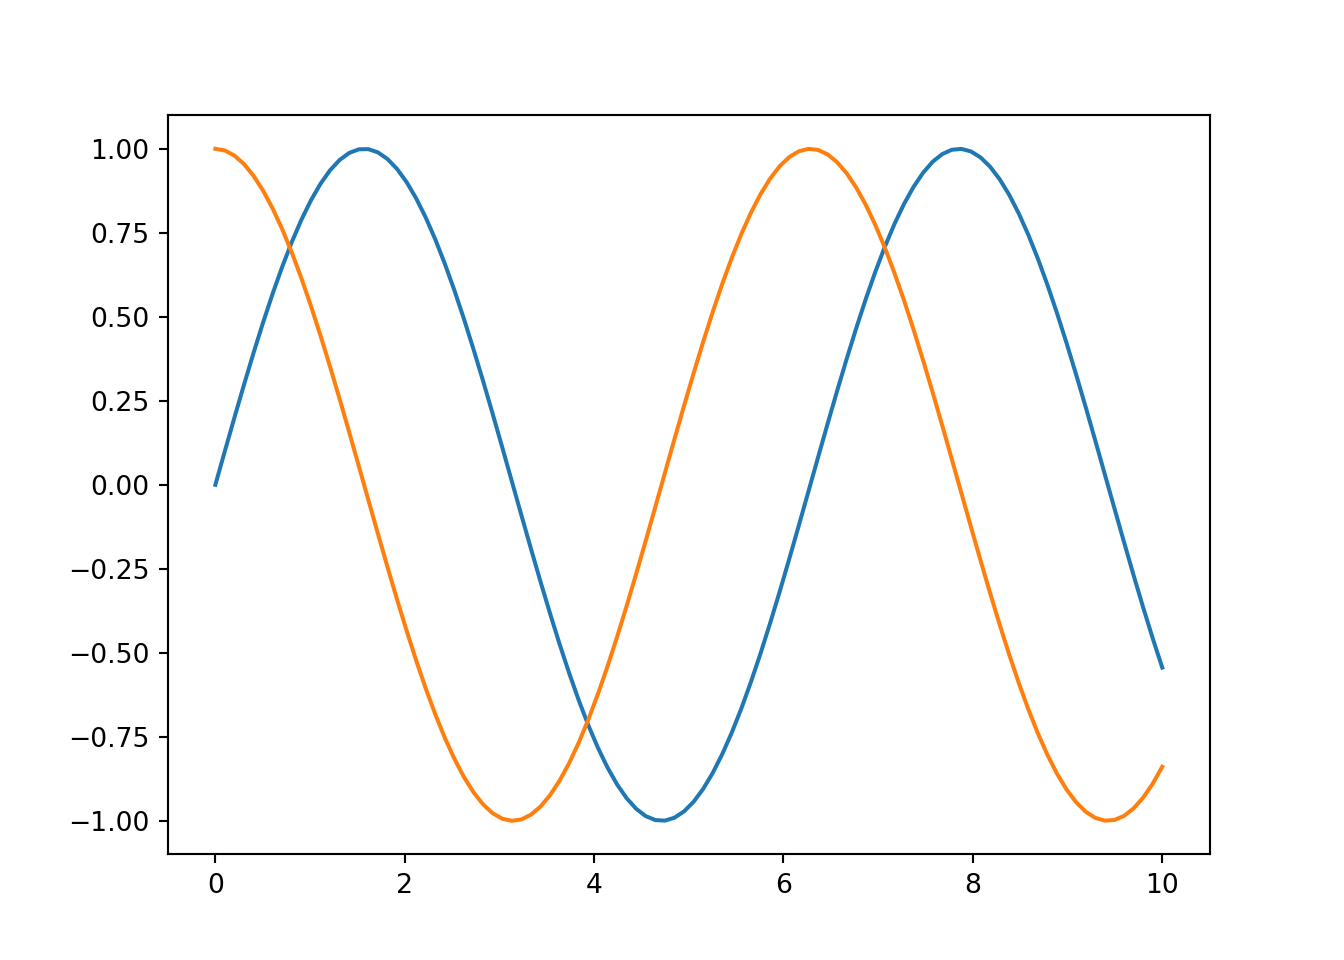
\includegraphics{t4ds/week6_files/figure-pdf/unnamed-chunk-4-1.pdf}

}

\end{figure}

\begin{Shaded}
\begin{Highlighting}[]
\NormalTok{plt.close()}
\end{Highlighting}
\end{Shaded}

Read data from sklearn and vizualize

\begin{Shaded}
\begin{Highlighting}[]
\ImportTok{import}\NormalTok{ matplotlib.pyplot }\ImportTok{as}\NormalTok{ plt}
\ImportTok{import}\NormalTok{ pandas }\ImportTok{as}\NormalTok{ pd}
\ImportTok{from}\NormalTok{ sklearn.datasets }\ImportTok{import}\NormalTok{ load\_iris }
\ImportTok{import}\NormalTok{ matplotlib}
\NormalTok{matplotlib.use(}\StringTok{\textquotesingle{}Agg\textquotesingle{}}\NormalTok{) }\CommentTok{\# To plot with Markdown}

\NormalTok{iris }\OperatorTok{=}\NormalTok{ load\_iris()}
\NormalTok{df\_iris }\OperatorTok{=}\NormalTok{ pd.DataFrame(iris.data)}
\NormalTok{df\_iris.columns }\OperatorTok{=}\NormalTok{ iris.feature\_names}

\CommentTok{\# Boxplot}
\NormalTok{plt.figure()}\OperatorTok{;}
\NormalTok{plt.boxplot(df\_iris)}
\end{Highlighting}
\end{Shaded}

\begin{verbatim}
{'whiskers': [<matplotlib.lines.Line2D object at 0x12dded3d0>, <matplotlib.lines.Line2D object at 0x12dded670>, <matplotlib.lines.Line2D object at 0x12ddfb580>, <matplotlib.lines.Line2D object at 0x12ddfb820>, <matplotlib.lines.Line2D object at 0x12de0a820>, <matplotlib.lines.Line2D object at 0x12de0aac0>, <matplotlib.lines.Line2D object at 0x12de19ac0>, <matplotlib.lines.Line2D object at 0x12de19d60>], 'caps': [<matplotlib.lines.Line2D object at 0x12dded910>, <matplotlib.lines.Line2D object at 0x12ddedbb0>, <matplotlib.lines.Line2D object at 0x12ddfbac0>, <matplotlib.lines.Line2D object at 0x12ddfbd60>, <matplotlib.lines.Line2D object at 0x12de0ad60>, <matplotlib.lines.Line2D object at 0x12de19040>, <matplotlib.lines.Line2D object at 0x12de27040>, <matplotlib.lines.Line2D object at 0x12de272e0>], 'boxes': [<matplotlib.lines.Line2D object at 0x12dded130>, <matplotlib.lines.Line2D object at 0x12ddfb2e0>, <matplotlib.lines.Line2D object at 0x12de0a580>, <matplotlib.lines.Line2D object at 0x12de19820>], 'medians': [<matplotlib.lines.Line2D object at 0x12ddede50>, <matplotlib.lines.Line2D object at 0x12de0a040>, <matplotlib.lines.Line2D object at 0x12de192e0>, <matplotlib.lines.Line2D object at 0x12de27580>], 'fliers': [<matplotlib.lines.Line2D object at 0x12ddb5a90>, <matplotlib.lines.Line2D object at 0x12de0a2e0>, <matplotlib.lines.Line2D object at 0x12de19580>, <matplotlib.lines.Line2D object at 0x12de27820>], 'means': []}
\end{verbatim}

\begin{Shaded}
\begin{Highlighting}[]
\NormalTok{plt.xticks([}\DecValTok{1}\NormalTok{, }\DecValTok{2}\NormalTok{, }\DecValTok{3}\NormalTok{, }\DecValTok{4}\NormalTok{], iris.feature\_names)}
\end{Highlighting}
\end{Shaded}

\begin{verbatim}
([<matplotlib.axis.XTick object at 0x12ddb52e0>, <matplotlib.axis.XTick object at 0x12ddb52b0>, <matplotlib.axis.XTick object at 0x12ddd9e50>, <matplotlib.axis.XTick object at 0x12de279d0>], [Text(1, 0, 'sepal length (cm)'), Text(2, 0, 'sepal width (cm)'), Text(3, 0, 'petal length (cm)'), Text(4, 0, 'petal width (cm)')])
\end{verbatim}

\begin{Shaded}
\begin{Highlighting}[]
\NormalTok{plt.grid()}
\NormalTok{plt.show()}
\end{Highlighting}
\end{Shaded}

\begin{figure}[H]

{\centering 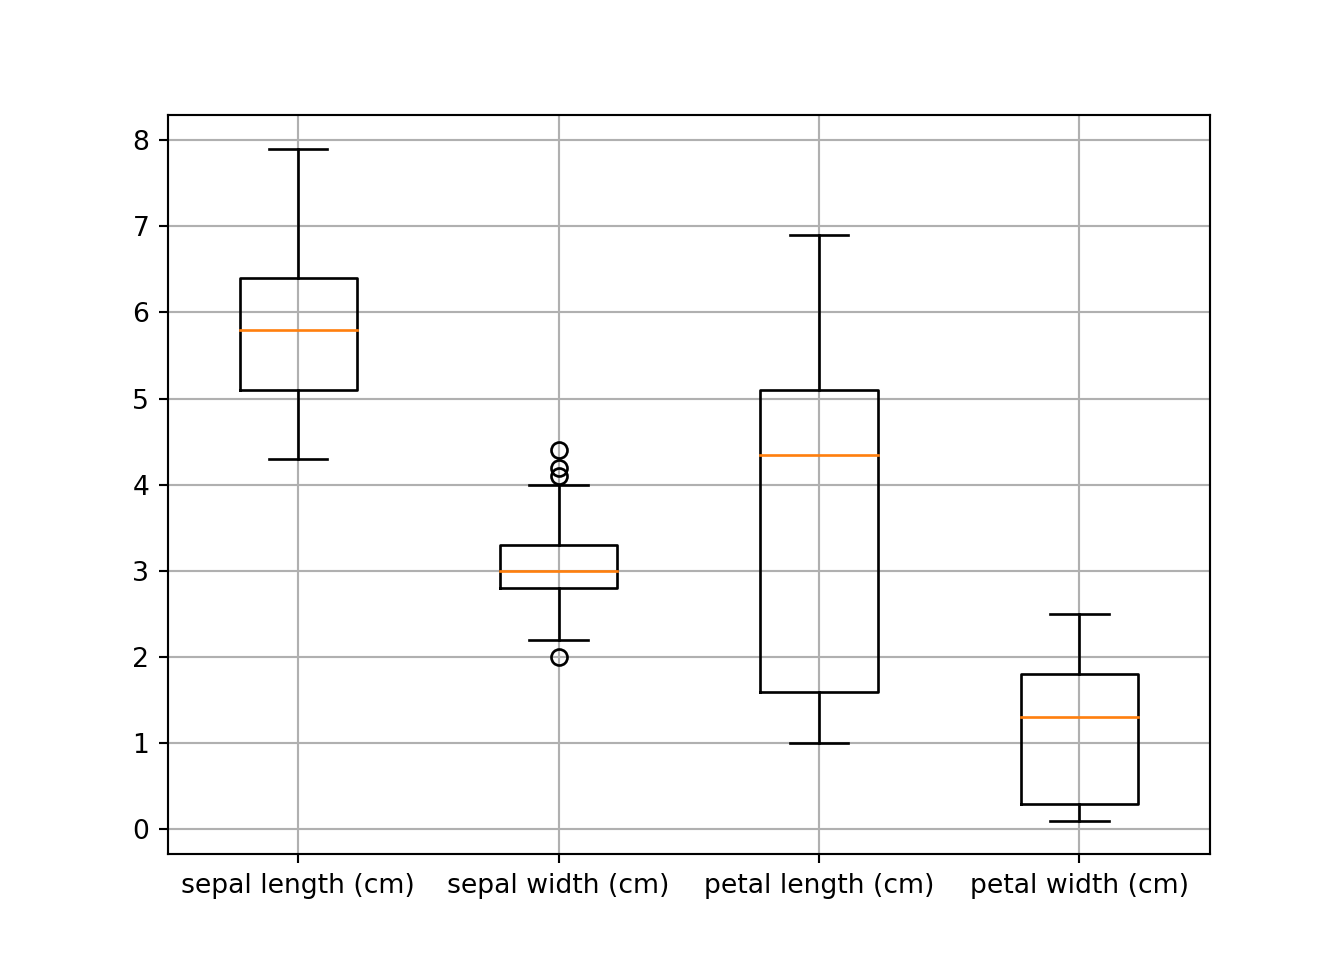
\includegraphics{t4ds/week6_files/figure-pdf/unnamed-chunk-5-3.pdf}

}

\end{figure}

\begin{Shaded}
\begin{Highlighting}[]
\NormalTok{plt.close()}

\CommentTok{\#  histogram}
\NormalTok{plt.figure()}\OperatorTok{;}
\NormalTok{plt.hist(df\_iris.iloc[:,}\DecValTok{0}\NormalTok{])}
\end{Highlighting}
\end{Shaded}

\begin{verbatim}
(array([ 9., 23., 14., 27., 16., 26., 18.,  6.,  5.,  6.]), array([4.3 , 4.66, 5.02, 5.38, 5.74, 6.1 , 6.46, 6.82, 7.18, 7.54, 7.9 ]), <BarContainer object of 10 artists>)
\end{verbatim}

\begin{Shaded}
\begin{Highlighting}[]
\NormalTok{plt.show()}
\end{Highlighting}
\end{Shaded}

\begin{figure}[H]

{\centering 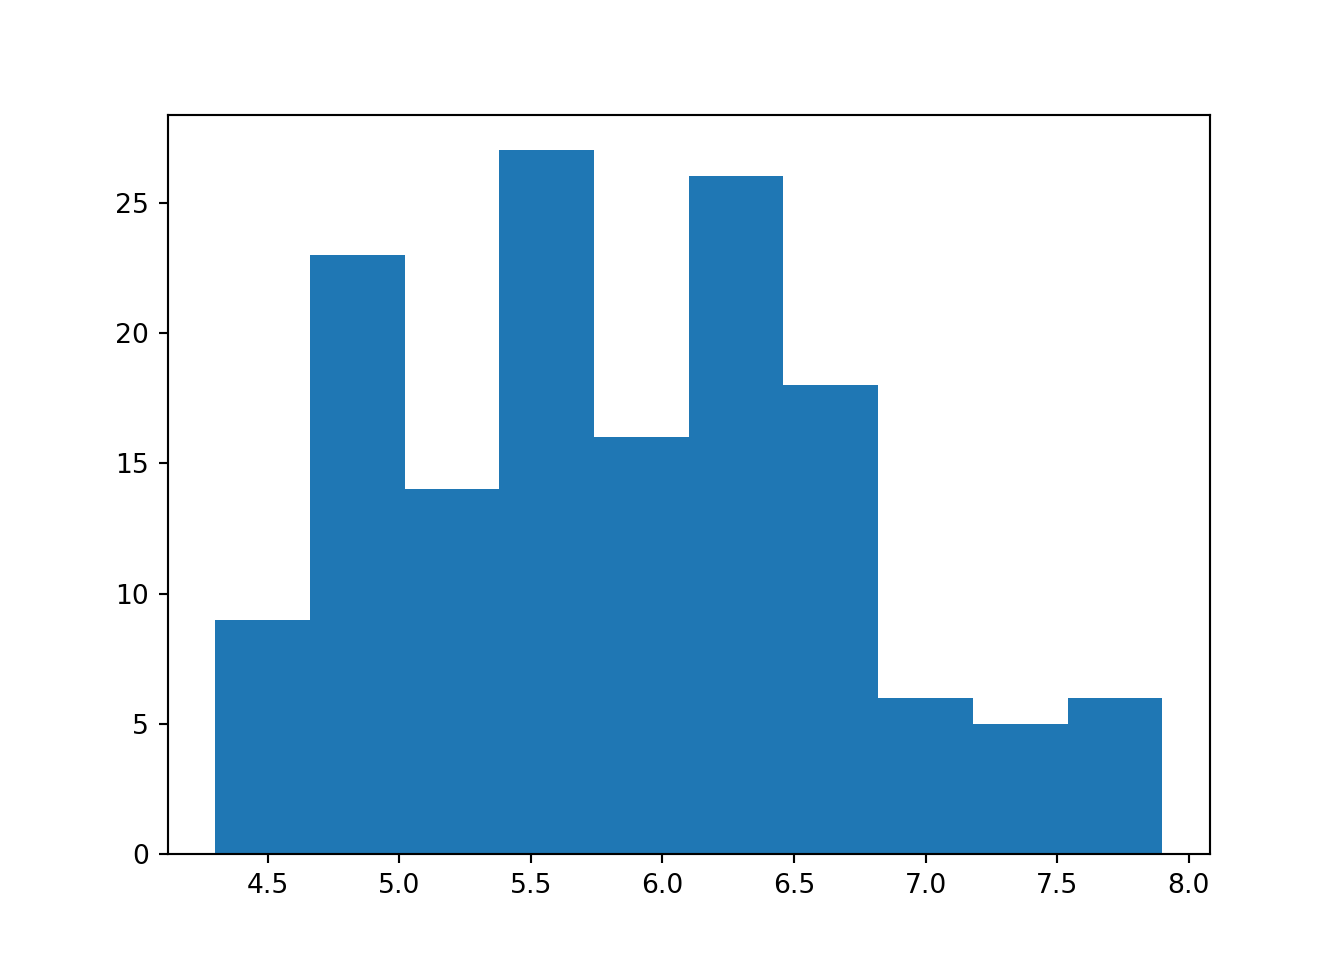
\includegraphics{t4ds/week6_files/figure-pdf/unnamed-chunk-5-4.pdf}

}

\end{figure}

\begin{Shaded}
\begin{Highlighting}[]
\NormalTok{plt.close()}
\end{Highlighting}
\end{Shaded}

🛎 🎙️ Recordings on Canvas will cover more details and examples! Have fun
learning and coding 😃! Let me know how I can help!

\hypertarget{assignment---python-statmlviz}{%
\section*{📚 👈 Assignment - Python
Stat/ML/Viz}\label{assignment---python-statmlviz}}
\addcontentsline{toc}{section}{📚 👈 Assignment - Python Stat/ML/Viz}

\markright{📚 👈 Assignment - Python Stat/ML/Viz}

Instructions are posted on Canvas.

\hypertarget{final-project}{%
\chapter*{Final Project}\label{final-project}}
\addcontentsline{toc}{chapter}{Final Project}

\markboth{Final Project}{Final Project}

\hypertarget{final-exam-project}{%
\section*{📚 👈 Final Exam Project}\label{final-exam-project}}
\addcontentsline{toc}{section}{📚 👈 Final Exam Project}

\markright{📚 👈 Final Exam Project}

Final Project instructions are posted on Canvas.

\hypertarget{references-1}{%
\chapter*{References}\label{references-1}}
\addcontentsline{toc}{chapter}{References}

\markboth{References}{References}

\hypertarget{refs}{}
\begin{CSLReferences}{1}{0}
\leavevmode\vadjust pre{\hypertarget{ref-Allenpython}{}}%
Downey, Allen. 2015. \emph{Think Python How to Think Like a Computer
Scientist}. Green Tea Press Needham, Massachusetts.

\leavevmode\vadjust pre{\hypertarget{ref-grolemund2014hands}{}}%
Grolemund, Garrett. 2014. \emph{Hands-on Programming with r: Write Your
Own Functions and Simulations}. " O'Reilly Media, Inc.".

\leavevmode\vadjust pre{\hypertarget{ref-databaser2020}{}}%
John David, Smith, Yang Sophie, Borasky M. Edward (Ed), Tyhurst Jim,
Came Scott, Thygesen Mary Anne, and Frantz Ian. 2020. \emph{Exploring
Enterprise Databases with r: A Tidyverse Approach}.
\url{https://smithjd.github.io/sql-pet/}.

\leavevmode\vadjust pre{\hypertarget{ref-luraschi2019mastering}{}}%
Luraschi, Javier, Kevin Kuo, and Edgar Ruiz. 2019. \emph{Mastering Spark
with r: The Complete Guide to Large-Scale Analysis and Modeling}.
O'Reilly Media.

\leavevmode\vadjust pre{\hypertarget{ref-rogel2018data}{}}%
Rogel-Salazar, Jesus. 2018. \emph{Data Science and Analytics with
Python}. CRC Press.

\leavevmode\vadjust pre{\hypertarget{ref-Jake2016python}{}}%
VanderPlas, Jake. 2016. \emph{Python Data Science Handbook}. O'Reilly
Media, Inc.

\leavevmode\vadjust pre{\hypertarget{ref-tidy-data}{}}%
Wickham, Hadley. 2014. {``Tidy Data.''} \emph{The Journal of Statistical
Software} 59. \url{http://www.jstatsoft.org/v59/i10/}.

\leavevmode\vadjust pre{\hypertarget{ref-wickham2016r}{}}%
Wickham, Hadley, and Garrett Grolemund. 2016. \emph{R for Data Science:
Import, Tidy, Transform, Visualize, and Model Data}. " O'Reilly Media,
Inc.".

\leavevmode\vadjust pre{\hypertarget{ref-zhang2017practical}{}}%
Zhang, Preston. 2017. \emph{Practical Guide for Oracle SQL, t-SQL and
MySQL}. CRC Press.

\end{CSLReferences}



\end{document}
